\documentclass[a4paper,12pt]{article}
\usepackage{amsthm
,amssymb,amsmath
}
\makeatletter
\renewcommand\section{\@startsection {section}{1}{\z@}%
                                   {-3.5ex \@plus -1ex \@minus -.2ex}%
                                   {2.3ex \@plus.2ex}%
                                   {\normalfont\large\bfseries}}
\makeatother
% \usepackage[top=3cm,right=3cm,bottom=2.5cm,left=2.5cm]{geometry}                 
\usepackage[colorlinks=true,linkcolor=blue,citecolor=red]{hyperref}  
\usepackage{xepersian}
\settextfont{XB Niloofar}
\setdigitfont{XB Zar}
\defpersianfont\kayhan{XB Kayhan}
\newcommand{\پ}{پروژه/پایان‌نامه/رساله }
\title{راهنمای  نوشتن \پ با استفاده از کلاس
\lr{SBU\_thesis} 
\author{\textbf{امیر حسین شرفی}
}\\
{\small دانشگاه شهید بهشتی، گروه ریاضی محض}
}
\date{}
\begin{document}
\maketitle
\baselineskip=.7cm
\tableofcontents
\newpage
\section{مقدمه}
این راهنما تغییر یافته‌ی راهنمایی است که آقای دامن‌افشان برای
\verb!Tabriz_thesis!
 نوشته‌اند.

همانطور که می‌دانید حروف‌چینی پروژه کارشناسی، پایان‌نامه یا رساله یکی از موارد پرکاربرد استفاده از زی‌پرشین است. از طرفی، یک پروژه، پایان‌نامه یا رساله،  احتیاج به تنظیمات زیادی از نظر صفحه‌آرایی  دارد که ممکن است برای
یک کاربر مبتدی، مشکل باشد. به همین خاطر، برای راحتی کار کاربر، یک کلاس با نام 
\verb!SBU!
 برای حروف‌چینی پروژه‌ها، پایان‌نامه‌ها و رساله‌های دانشگاه تبریز با استفاده از نرم‌افزار زی‌پرشین،  آماده شده است. این فایل به 
گونه‌ای طراحی شده است که کلیه خواسته‌های مورد نیاز  مدیریت تحصیلات تکمیلی دانشگاه شهید بهشتی را برآورده می‌کند و نیز، حروف‌چینی بسیاری
از قسمت‌های آن، به طور خودکار انجام می‌شود.

کلیه فایل‌های لازم برای حروف‌چینی با کلاس گفته شده، داخل پوشه‌ای به نام
\verb!SBU_thesis!
  قرار داده شده است. توجه داشته باشید که برای استفاده از این کلاس باید فونت‌های
  \verb!Niloofar XB!،
 \verb!Yas!،
  \verb!IranNastaliq!
  و
    \verb!Titre XB!
    روی سیستم شما نصب شده باشد.
\section{این همه فایل؟!}\label{sec2}
از آنجایی که یک پایان‌نامه یا رساله، یک نوشته بلند محسوب می‌شود، لذا اگر همه تنظیمات و مطالب پایان‌نامه را داخل یک فایل قرار بدهیم، باعث شلوغی
و سردرگمی می‌شود. به همین خاطر، قسمت‌های مختلف پایان‌نامه یا رساله را داخل فایل‌های جداگانه قرار داده‌ایم. مثلاً تنظیمات پایه، داخل فایل
\verb!SBU.cls!، 
تنظیمات قابل تغییر توسط کاربر، داخل 
\verb!commands.tex!،
قسمت مشخصات فارسی پایان‌نامه، داخل 
\verb!fa_title.tex!،
مطالب فصل اول، داخل 
\verb!chapter1!
و ... قرار داده شده است. نکته بسیار مهمی که در اینجا وجود دارد این است که از بین این همه فایل، فقط فایل اصلی، یعنی
\verb!main.tex!
قابل اجرا است. یعنی بعد از تغییر فایل‌های دیگر، برای دیدن نتیجه تغییرات، باید این فایل را اجرا کرد. بقیه فایل‌ها به این فایل، کمک می‌کنند تا بتوانیم خروجی کار را ببینیم. اگر به فایل 
\verb!main.tex!
دقت کنید، متوجه می‌شوید که قسمت‌های مختلف پایان‌نامه، توسط دستورهایی مانند 
\verb!input!
و
\verb!include!
به فایل اصلی، یعنی 
\verb!main.tex!
معرفی شده‌اند. بنابراین، فایلی که همیشه با آن سروکار داریم، فایل 
\verb!main.tex!
است.
در این فایل، فرض شده است که پایان‌نامه یا رساله شما، از ۳ فصل و یک پیوست، تشکیل شده است. با این حال، اگر
  پایان‌نامه یا رساله شما، بیشتر از ۳ فصل و یک پیوست است، باید خودتان فصل‌های بیشتر را به این فایل، اضافه کنید. این کار، بسیار ساده است. فرض کنید بخواهید یک فصل دیگر هم به پایان‌نامه، اضافه کنید. برای این کار، کافی است یک فایل با نام 
\verb!chapter4!
و با پسوند 
\verb!.tex!
بسازید و آن را داخل پوشه 
\verb!SBU_thesis!
قرار دهید و سپس این فایل را با دستور 
\verb!% !TeX root=main.tex
\chapter{بررسی نتایج و نتیجه‌گیری‌}
در این فصل به بررسی نتایج رویکرد ارائه شده و مقایسه‌ی آن با سایر روش‌های پیش‌بینی خواهیم پرداخت و در آخر نتیجه‌گیری و جمع‌بندی کلی ارائه خواهیم کرد.
\section{ روش جامع اعتبارسنجی متقابل k برابری
\label{K-fold CV}}
 
روش جامع اعتبارسنجی متقابل k برابری
\LTRfootnote{k-Fold Cross Validation (K-fold CV)}
رویکردی تثبیت شده برای اعتبارسنجی قدرت الگوریتم‌ها در یادگیری ماشین است.  برای نشان دادن این واقعیت که داروهای جدید چه نوع برهم‌کنشی دارند و برای جلوگیری از پیش‌بینی بیش از حد خوش‌بینانه، اعتبارسنجی متقابل باید به‌طور دقیق طراحی شود. برای جفت داروهایی که هیچ  برهم‌کنشی شناخته شده‌ای ندارند، اعتبارسنجی متقابل سعی در پیش‌بینی نوع برهم‌کنشی جدید بین آنها و داروهای دارای برهم‌کنش شناخته شده دارد. تولید نمونه‌های آموزش و آزمایش به شرح زیر است:

کل مجموعه داده‌ها به k قسمت مساوی تقسیم می‌شوند. k-1 قسمت به عنوان مجموعه داده‌های آموزشی استفاده می‌شود و براساس آن مدل ساخته می‌شود و با یک قسمت باقی‌مانده عملیات ارزیابی انجام می‌شود. فرآیند مزبور به تعداد k مرتبه تکرار خواهد شد، به گونه‌ای که از هر کدام از k قسمت تنها یکبار برای ارزیابی استفاده شده و در هر مرتبه یک دقت
\LTRfootnote{Precision}
برای مدل ساخته شده، محاسبه می‌شود. در این روش ارزیابی دقت نهایی دسته‌بند
\LTRfootnote{Classifier}
برابر با میانگین k دقت محاسبه شده خواهد بود. معمول‌ترین مقداری که در متون علمی برای k در نظر گرفته می‌شود برابر با 5 یا 10 می‌باشد. بدیهی است هر چه مقدار k بزرگتر شود، دقت محاسبه شده برای دسته‌بند قابل اعتماد‌تر بوده و دانش حاصل شده جامع‌تر خواهد بود و البته افزایش زمان ارزیابی دسته‌بند نیز افزایش می یابد که مهم‌ترین مشکل محسوب می‌شود. هر تنظیم و هر مجموعه داده، اعتبارسنجی مختص خود را دارد. در این پایان نامه با توجه به نوع مسئله و روش‌های به‌کارگرفته شده، از دو اعتبارسنجی متقابل 10 برابری متفاوت به منظور تقسیم کردن داده‌ها به دو مجموعه ارزیابی و آموزش در نظر گرفته‌شد که عبارتند از:

\textbf{حالت اول: اعتبارسنجی متقابل 10 برابری بدون برهم‌کنش‌های ناشناخته}

در این حالت 90 درصد از برهم‌کنش‌های مثبت و منفی را به‌طور تصادفی
\LTRfootnote{Random}
انتخاب می‌کنیم. برای مجموعه‌ی ارزیابی نیز 10 درصد باقی‌مانده از برهم‌کنش‌های مثبت و منفی در نظر می‌گیریم. 

در روال اعتبارسنجی حالت اول مدل انتخاب شده و بعضی پارامترهای اساسی، همچون تعداد ایپوک، تعیین مقدار شد. شکل
\ref{ModelSelection}
روند آموزش مدل انتخابی را نشان می‌دهد. طبق انتظار صحت مدل روی داده‌های آموزش صعودی اکید است اما برای داده‌های اعتبارسنجی بعد از ایپوک ۵ فراز و فرودهایی دیده می‌شود.

در نمودار تابع خطا، تا پایان ایپوک ۵، با افزایش ایپوک‌ها، مقدار تابع خطای مدل روی داده‌های آموزش و رو‌ی داده‌های اعتبارسنجی کم می‌شود. بعد از ایپوک ۵ روند مدل روی داده‌های آموزشی ادامه می‌یابد اما روند برروی داده‌های اعتبارسنجی برعکس می‌شود. به‌معنای دیگر بیش‌برازش رخ می‌دهد. لذا براساس نمودارها تعداد ایپوک مناسب در این مرحله ۵ درنظر گرفته‌شد.

\begin{figure}[!h]
	%\centering
	\begin{minipage}[b]{0.99\linewidth} 
    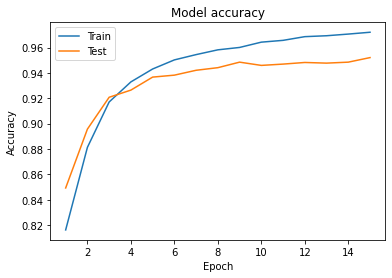
\includegraphics[width=.55\textwidth]{section4/ModelSelection/selectedModelAcc.png} 
    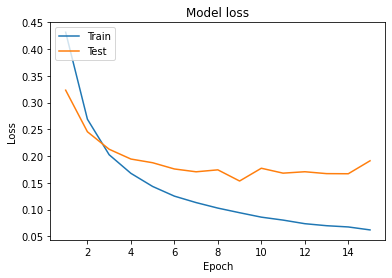
\includegraphics[width=.55\textwidth]{section4/ModelSelection/selectedModelLoss.png} 
\end{minipage}
	\caption{موارد صحت و مقادیر تابع خطا برای شماره ایپوک‌های مختلف}
در شکل راست صحت مدل روی داده‌های آموزش و اعتبارسنجی در طی ۱۵ ایپوک نشان داده می‌شود و در شکل چپ مقادیر تابع خطا در ایپوک‌های مختلف مشاهده می‌شود.
	\label{ModelSelection}
\end{figure}


\textbf{
حالت دوم:اعتبارسنجی متقابل 10 برابری همراه با برهم‌کنش‌های ناشناخته}

در این حالت مجموعه همه برهم‌کنش‌ها (مثبت، منفی، صفرهای مرحله اول) را به 10 دسته مساوی تقسیم می‌کنیم. یک دسته را به‌عنوان مجموعه ارزیابی و 9 دسته دیگر را به‌عنوان مجموعه‌ داده‌ی آموزش درنظر می‌گیریم. همه صفرهای مرحله‌ی قبل را هم به 10 قسمت تقسیم کرده و به نسبت ۱ به ۹ هم به مجموعه‌ی ارزیابی و هم به مجموعه‌ی آموزش اضافه می‌کنیم.

در روال اعتبارسنجی حالت دوم مدل پیشین با کم‌ترین تغییرات برای پیش‌بینی سه‌کلاسه آموزش داده ‌شد. علاوه‌براین، پارامتر اساسی تعداد ایپوک، تعیین مقدار شد. شکل
\ref{lastTripleModel}
روند آموزش را نشان می‌دهد. روند صحت مدل روی داده‌های آموزش با افزایش ایپوک‌ها صعودی اکید است اما برای داده‌های اعتبارسنجی، مدل بعد از ایپوک ۹ مقدار صحت ثابت و کمی افول می‌کند.

در نمودار تابع خطا، تا پایان ایپوک ۹، با افزایش ایپوک‌ها، مقدار تابع خطای مدل روی داده‌های آموزش و رو‌ی داده‌های اعتبارسنجی کم می‌شود. بعد از ایپوک ۹ روند مدل روی داده‌های آموزشی ادامه می‌یابد اما روند برروی داده‌های اعتبارسنجی گاهی بالا و گاهی پایین می‌رود. بدان معناست که احتمال بیش‌برازش بعد از ایپوک ۹ وجود دارد. لذا براساس نمودارها تعداد ایپوک مناسب برای مدل پیش‌بینی سه‌کلاسه ۹ می‌باشد.
\begin{figure}[!h]
%\centering
\begin{minipage}[b]{0.99\linewidth}
    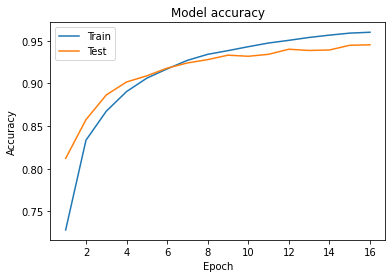
\includegraphics[width=.55\textwidth]{section4/lastTripleModel/modelTripleACC.png}
    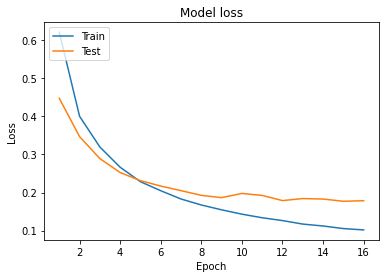
\includegraphics[width=.55\textwidth]{section4/lastTripleModel/modelTripleLoss.png}
\end{minipage}
	\caption{نمودار صحت و مقادیر تابع خطا برای شماره ایپوک‌های مختلف}
در شکل راست صحت مدل روی داده‌های آموزش و اعتبارسنجی در طی ۱۶ ایپوک نشان داده می‌شود و در شکل چپ مقادیر تابع خطا در ایپوک‌های مختلف مشاهده می‌شود.
\label{lastTripleModel}
\end{figure}

\section{معرفی معیارهای سنجش}

به‌ منظور مقایسه عملکرد روش خود با سایر روش‌های موجود، از چهار معیار سنجش، 
$F_{measure}$،
صحت
\LTRfootnote{Accuracy}،
مساحت زیر نمودار منحنی مشخصه‌ی عملکرد سیستم (AUC)
\LTRfootnote{Area Under Roc Curve}
و مساحت زیر نمودار بازخوانی-دقت (AUPR) 
\LTRfootnote{Area Under Precision-Recall Curve}
استفاده شده ‌است. برای تعریف این معیار ها ابتدا چهار معیار شمارشی در این زمینه را در جدول 
\ref{f1}
معرفی کرده‌ایم.
\begin{table}[h!]
\centering 
\begin{tabular}{|c|c|c|c|}
\hline
& پیش‌بینی برهم‌کنش مثبت	& 
پیش‌بینی برهم‌کنش منفی 
\\
\hline
در واقعیت برهم‌کنش مثبت	& مثبت درست& منفی نادرست
\\
\hline
در واقعیت برهم‌کنش منفی& مثبت نادرست & منفی درست
 \\\hline
 \end{tabular}
	\caption{
حالت‌های ممکن نتایج یک یادگیری ماشین 
}
	\label{f1}
\end{table}

با استفاده از آن‌ها چهار معیار سنجش به ترتیب زیر تعریف می‌شوند:

\textbf{صحت:}
نسبت نتایج واقعی (مثبت درست و منفی درست) به تمام موارد مورد بررسی است. 

$$ \mbox{صحت} =  \frac{ \mbox{\rl{تعداد مثبت های درست}} + \mbox{\rl{تعداد منفی های درست}}}
{\mbox{\rl{ تعداد کل نمونه ها}}} $$


همان‌طور که از رابطه بالا مشخص است، حاصل‌جمع تعداد مثبت‌های درست و تعداد منفی‌های درست، نشانگر تعداد نمونه‌هایی است که توسط سیستم به‌درستی تشخیص داده شده‌اند.  مشکل استفاده از معیار صحت، این است که این معیار در زمانی که داده‌ها نامتوازن هستند، معیار مناسبی نیست. زیرا در این حالت، رده‌های را که در بین داده‌ها بیشترین آرا را دارد(رده اکثریت) را به تمام داده‌ها نسبت می‌دهد.

\textbf{$F_{measure}$:}
یک میانگین هارمونیک
\LTRfootnote{Harmonic Average}
میان پارامترهای فراخوانی و دقت می‌باشد و هدف اصلی بیشینه کردن این معیار می‌باشد. 
$F_{measure}$
بر اساس رابطه‌ی زیر محاسبه می‌شود.

$$ F_{measure}  =  \frac{ 2\times( \mbox{\rl{دقت}} + \mbox{\rl{فراخوانی}})}
{\mbox{\rl{ دقت}} + \mbox{\rl{فراخوانی}}} $$

هر کدام از معیارهای فراخوانی
\LTRfootnote{Recall}
و دقت نیز طبق رابطه‌های زیر محاسبه می‌شوند.


$$ \mbox{دقت} =  \frac{\mbox{\rl{تعداد مثبت های درست}}}
{\mbox{\rl{تعداد مثبت های درست}} + \mbox{\rl{تعداد منفی های نادرست}}} $$


$$ \mbox{فراخوانی} =  \frac{ \mbox{\rl{تعداد مثبت های درست}}}
{\mbox{\rl{تعداد مثبت های درست}} + \mbox{\rl{تعداد مثبت های نادرست}}} $$


\textbf{مساحت زیر نمودار بازخوانی-دقت:}
نمودار بازخوانی-دقت یک منحنی دو بعدی است که در آن دقت روی محور عرض‌ها و به‌طور مشابه فراخوانی روی محور طول‌ها رسم می‌شوند. به‌بیان دیگر منحنی دقت-فراخوانی مصالحه نسبی میان دقت و فراخوانی در آستانه‌های متفاوت را نشان می‌دهد. سطح زیر این نمودار یکی از مهم‌ترین معیارهای ارزیابی مدل می‌باشد.
 
\textbf{مساحت زیر نمودار منحنی مشخصه‌ی عملکرد سیستم:}
منحنی‌های مشخصه‌ی عملکرد سیستم، منحنی‌های دو بعدی هستند که در آن‌ها نرخ تشخیص صحیح دسته‌ی مثبت(TPR)
\LTRfootnote{True Positive Rate}
روی محور عرض‌ها و به‌طور مشابه نرخ تشخیص غلط دسته‌ی منفی(FPR)
\LTRfootnote{False Positive Rate }
روی محور طول‌ها رسم می‌شوند. به‌بیان دیگر یک منحنی مشخصه عملکرد سیستم مصالحه نسبی میان سودها و هزینه‌ها را نشان می‌دهد. فرمول‌های  نرخ تشخیص غلط دسته‌ی منفی و نرخ تشخیص صحیح دسته‌ی مثبت که در زیر آورده شده‌است، ماهیت این عناصر را روشن می‌کنند.
 
$$ \mbox{\rl{ نرخ تشخیص صحیح دسته مثبت}} =  \frac{ \mbox{\rl{تعداد مثبت های درست}}}
{\mbox{\rl{تعداد مثبت های درست}} + \mbox{\rl{تعداد منفی های نادرست}}} $$ 

 
$$ \mbox{\rl{ نرخ تشخیص صحیح دسته منفی}} =  \frac{ \mbox{\rl{تعداد مثبت های نادرست}}}
{\mbox{\rl{تعداد مثبت های نادرست}} + \mbox{\rl{تعداد منفی های  درست}}} $$ 


\section{مقایسه‌ی نتایج}
طی روال اعتبارسنجی مبسوط در بخش 
\ref{K-fold CV}
مدل تشخیص نوع برهم‌کنش انتخاب و آموزش داده ‌شد. سپس با تشخیص عدم برهم‌کنش‌های محتمل‌تر مدل سه‌کلاسه نهایی ارائه شد. در ادامه برای بررسی قابلیت اطمینان، استواری و کارایی، مدل
\lr{SNF-CNN}
در روال اعتبارسنجی برروی داده آزموده شد. نتایج
\lr{SNF-CNN}
و سایر روش‌ها که برای مقایسه در نظر گرفته شده‌اند، در این بخش ارائه شده و بررسی می‌شوند. قبل از مقایسه‌ی روش‌های مختلف، نمونه‌ای از نتایج اجرای شبکه‌ی عصبی برای تشخیص نوع برهم‌کنش کاهنده و افزاینده ارائه می‌شود.

\begin{table}[h!]
\centering
\begin{tabular}{|c|c|c|c|c|}
\hline
 
تعداد & $F_{score}$ &فراخوانی & دقت&  
\\
\hline

850 & 0/88 & 0/83 & 0/94 & کاهنده
\\
\hline

3052 & 0/97 & 0/99 & 0/95 & افزاینده
\\
\hline

3902 & 0/95 &  &  & صحت 
\\
\hline
 
3902 & 0/93 & 0/91 & 0/95 & \lr{Macro Avg}
\\
\hline

 3902 & 0/95& 0/95 & 0/95 & \lr{Weighted Avg}
\\
\hline
\end{tabular}
	\caption{
گزارش دسته‌بندی نوع برهم‌کنش}
	\label{classificatonReport}
\end{table}

جدول 
\ref{classificatonReport}
 مثالی از نتایج اجرای مدل است که توانایی مدل از جهت دقت، بازخوانی و 
$F_{score}$
در تشخیص نوع برهم‌کنش‌ها نشان می‌دهد. براساس جدول 
\ref{classificatonReport}
دقت مدل در تشخیص برهم‌کنش افزاینده و کاهنده ۹۵ و ۹۴ درصد است درحالی که فراخوانی به ترتیب ۹۹ و ۸۳ درصد می‌باشد. مقدار 
$F_{measure}$
نیز ۹۷ و ۸۸  درصد می‌باشد که توانایی بالاتر مدل در تشخیص برهم‌کنش‌های افزاینده از تعداد بالاتر این نوع برهم‌کنش‌ها می‌آید. نسبت برهم‌کنش افزاینده به کاهنده تقریبا ۴ به ۱ است. 

\begin{table}[h!]
\centering
\begin{tabular}{|c|c|c|c|c|}
\hline
 
تعداد & $F_{score}$ &فراخوانی & دقت&  
\\
\hline

850 & 0/86 & 0/84 & 0/88 & کاهنده
\\
\hline

3000 & 0/96 & 0/95 & 0/96 & عدم برهم‌کنش
\\
\hline

3052 & 0/96 & 0/97 & 0/95 & افزاینده
\\
\hline

6902 & 0/95 &  &  & صحت 
\\
\hline
 
6902 & 0/93 & 0/92 & 0/93 & \lr{Macro Avg}
\\
\hline

 6902 & 0/95& 0/95 & 0/95 & \lr{Weighted Avg}
\\
\hline
\end{tabular}
	\caption{
گزارش دسته‌بندی حالت سه‌کلاسه برهم‌کنش}
	\label{TripleclassificatonReport}
\end{table}
همچنین در جدول 
\ref{TripleclassificatonReport}
گزارش دسته‌بندی برای حالت سه‌کلاسه نشان داده می‌شود. در این اجرا دقت مدل برای تشخیص برهم‌کنش افزاینده، بدون برهم‌کنش و برهم‌کنش کاهنده به ترتیب ۹۵، ۹۶ و ۸۸ درصد است. فراخوانی به ترتیب ۹۷، ۹۵ و ۸۴ درصد است و در نهایت 
$F_{measure}$
۹۶، ۹۶ و ۸۶ درصد می‌باشد. مشاهده شد، توان مدل در حالت سه‌کلاسه مقدار کمی نسبت به دوکلاسه کاهش می‌یابد که می‌تواند دو دلیل داشته ‌باشد.

۱) مسئله سه‌کلاسه از دوکلاسه سخت‌تر است.

۲) صفرها یا عدم برهم‌کنش‌ها لزوما واقعی نبوده و از نظر داروشناسی تایید شده نیستند پس احتمال وجود مقداری اختلال می‌رود.

لذا به دلایل فوق الذکر مقداری کاهش توان مدل در تشخیص سه‌کلاسه دور از انتظار نبود.

از آنجا که الگوریتم‌های پیشین در پیش‌بینی سه‌تایی برهم‌کنش دارو-دارو از 
\lr{AUC}
و 
\lr{AUPR}
بهره می‌برند، لذا نتایج الگوریتم ارائه ‌شده براساس این دو معیار و برای تشخیص برهم‌کنش افزاینده، عدم برهم‌کنش و برهم‌کنش کاهنده مطابق جدول 
\ref{SNF-CNNresult}
می‌باشد. همچنین در جدول برای الگوریتم ارائه ‌شده این تحقیق بازه‌ی بالا و پایین با اطمینان ۹۵ درصد گزارش شده‌است که نشان می‌دهد، نتایج الگوریتم در روال اعتبارسنجی ۱۰تایی تغییرات کمی داشته و الگوریتم ارائه‌شده استوار بوده و قابل اعتماد می‌باشد.

\begin{table}[h!]
\centering 
\begin{tabular}{|c|c|c|c|}
\hline
& AUC	 & AUPR
\\
\hline
افزاینده	& $0/9747 \pm 0/0033$ & $0/9666 \pm 0/0045$
\\
\hline
کاهنده  & $0/9686 \pm 0/0028$ & $0/8221 \pm 0/0184$
\\
\hline
عدم برهم‌کنش & $0/9714 \pm 0/0040$ & $0/9480 \pm 0/0083$
\\\hline
 \end{tabular}
	\caption{
نتایج الگوریتم
\lr{SNF-CNN}
 در پیش‌بینی سه‌کلاسه براساس معیارهای 
\lr{AUC}
و 
\lr{AUPR}
و بازه‌ی اطمینان آن‌ها
}
	\label{SNF-CNNresult}
\end{table}


در جدول 
\ref{AUCAUPR}
نتایج الگوریتم
\lr{SNF-CNN}
برای سه حالت میانگین گرفته ‌شده و در جدول با دیگر الگوریتم‌های سه‌کلاسه موجود مقایسه ‌شده ‌است. طبق جدول 
\ref{AUCAUPR}
الگوریتم ارائه ‌شده اختلاف بالایی نسبت به دیگر الگوریتم‌های برتر مسئله‌ی سه‌تایی، داشته و توانسته الگوریتم‌های دیگر را به چالش بکشد.

\begin{table}[h!]
\centering 
\begin{tabular}{|c|c|c|c|}
\hline
& AUC	& AUPR 
\\
\hline
SNF-CNN	& 0/971 & 0/912
\\
\hline
\rl{\cite{Shi J2019}} BRSNMF & 0/645 & 0/346
\\
\hline
\rl{\cite{Yu H2018}} Semi-NMF & 0/796 & 0/579
\\
\hline
\rl{\cite{Shi J-Y2018}} TMFUF  & 0/842  & 0/526
 \\\hline
 \end{tabular}
	\caption{
مقایسه‌نتایج الگوریتم‌های پیش‌بینی سه‌کلاسه براساس معیارهای 
\lr{AUC}
و 
\lr{AUPR}
}
	\label{AUCAUPR}
\end{table}



\section{نتیجه‌گیری و جمع‌بندی}
در این رساله، با مدل‌سازی مسئله‌ی پیش‌بینی برهم‌کنش دارو-دارو و بهره‌گیری از رویکردهای مسئله‌ی سیستم‌های توصیه‌گر، روشی نوین با نتایج به مراتب بهتر نسبت به کارهای گذشته ارائه دادیم. با بررسی چهار معیار سنجش، صحت، مساحت زیر نمودار منحنی مشخصه‌ی عملکرد سیستم، مساحت زیر نمودار فراخوانی-دقت و 
$F_{measure}$
 دیدیم که روش ما نتایج دقیق‌تری نسبت به سایر روش‌های موجود ارائه می‌کند. همچنین برای بررسی میزان قدرت روش
\lr{SNF-CNN}
در شناسایی برهم‌کنش‌های ناشناخته، تعدادی از برهم‌کنش‌های جدید که مدل آنها را پیش‌بینی کرده است را مورد تحقیق قرار داده‌ایم.





!
داخل فایل
\verb!main.tex!
و بعد از دستور
\verb!% !TeX root=main.tex
\chapter{
پیش‌بینی برهم‌کنش دارو-داروی با رویکرد سیتم توصیه‌گر یادگیری عمیق
}

در این فصل، ابتدا داده‌ها و ویژگی‌ها معرفی می‌شوند. سپس الگوریتم جدیدی مبتنی بر ۱) ادغام شباهت‌های دارویی و ۲) سیستم‌های توصیه‌گر یادگیری عمیق برای پیش‌بینی برهم‌کنش دارو - دارو در حالت جامع سه کلاسه ارائه می‌شود. الگوریتم مذکور
\lr{SNF-CNN}
نامیده می‌شود که مخفف
\lr{Predicting Comperhensive Drug - Drug Interaction via Similarity Network Fusion and Convolutional Neural Networks}
است. در این الگوریتم ابتدا روند آماده‌سازی داده‌ها توضیح داده می‌شود و سپس سیستم توصیه‌گری طراحی و بروی برهم‌کنش‌‌‌های افزاینده و کاهنده آموزش داده ‌می‌شود که جفت دارو‌‌های بدون برهم‌کنش را، با احتمال بالا تشخیص می‌دهد. در ادامه سیستم توصیه‌گر قبلی که مبتنی بر شبکه‌ی عصبی کانولوشن است، برروی داده‌‌‌های برهم‌کنش افزاینده و کاهنده و بدون برهم‌کنش (تشخیص داده‌شده در مرحله‌ی قبل) آموزش داده می‌شود. نتایج در روند اعتبارسنجی متقابل 10 برابری
\LTRfootnote{10-fold CV}
ثبت و در فصل چهار تحلیل می‌شود.

\section{داده‌ها و ویژگی‌ها}

در این پژوهش از مجموعه داده‌ای که در مقاله
\cite{Yu H2018}
ارائه شده است، استفاده می‌شود. این مجموعه شامل 568 داروی کوچک مولکول تایید شده است که هر دارو حداقل یک برهم‌کنش با دیگر دارو‌‌های مجموعه دارد. درمجموع برهم‌کنش‌‌‌های بین این ۵۶۸ دارو شامل 21351 برهم‌کنش است، که متشکل از 16757 برهم‌کنش افزاینده و 4594 برهم‌کنش کاهنده می‌باشد. 

علاوه‌براین، هر دارو با دو بردار ویژگی ۸۸1 بعدی ساختار شیمیایی
$F_{str}$
 از 
\lr{PubChem}\cite{Y. Wang2009}
 و 9149 بعدی عوارض جانبی خارج از برچسب
$F_{se}$
 از 
\lr{OFFSIDES}\cite{Tatonetti2012}
 نشان ‌داده می‌شود. برای جزئیات بیشتر به بخش 
\ref{ProbelmDefine}
 مراجعه کنید. 

داروها و برهم‌کنش‌ها تشکیل گراف می‌دهند. در این گراف گره‌ها دارو و یال‌ها برهم‌کنش هستند. جزئیات مجموعه‌ی داده‌‌‌های برهم‌کنش در جدول
\ref{dataDetail}
 ذکر شده‌است.
\begin{table}[h!]
\centering
\begin{tabular}{|c|c|c|c|c|c|c|c|}
\hline
خصوصیت & مقدار & درجه & مقدار & درجه‌ی
\lr{E-DDI}
  &  مقدار  &  درجه‌ی
\lr{D-DDI}
 & مقدار
\\
\hline
تعداد دارو 
&568 &
میانگین
& ۷۵/۱۸
& میانگین
&۵۹/۰۰
& میانگین
 & ۱۶/۱۸
\\
\hline
تعداد 
\lr{DDI}
&21351 &
میانه
& ۶۱/۵۰
&میانه
&۴۵/۰۰
&میانه
 & ۸/۰۰
\\
\hline

تعداد 
\lr{E-DDI}
 & 16757 &
بیشینه
& ۲۹۶
& بیشینه
&۲۳۰
&  بیشینه
 & ۲۰۶
\\
\hline
 
تعداد 
\lr{D-DDI}
 & 4594 &
 کمینه
& ۱
& کمینه
&0
& کمینه
 & ۰
\\
\hline
\end{tabular}
	\caption{
جزئیات مجموعه‌ی داده‌‌‌های برهم‌کنش
\cite{Yu H2018}
}
	\label{dataDetail}
\end{table}

\section{مدل‌سازی مسئله
\label{ProbelmDefine}} 

 
$D={\lbrace d_i \rbrace} , i=1,2,3,...,m$
را به‌عنوان مجموعه‌ای از
\lr{m}
داروی تایید شده دارای برهم‌کنش تعریف می‌کنیم. برهم‌کنش بین
\lr{m}
داروی تایید شده را به‌صورت یك ماتریس مجاورت متقارن
\LTRfootnote{Symmetric Adjacency Matrix }
$A_{m\times m}={\lbrace a_{ij} \rbrace}$
در نظر می‌گیریم كه
\lr{m}
تعداد داروها می‌باشد و
$a_{ij}$
هر درآیه از ماتریس
\lr{A}
است. برای مقادیر 
$a_{ij}$
دو دیدگاه متفاوت وجود دارد: 


الف) دیدگاه دوکلاسه 
\LTRfootnote{Binary Approach}:
$a_{ij}=1$
 اگر دارو‌‌های 
\lr{i}
ام و 
\lr{j}
ام تاثیر متقابل شناخته شده داشته باشند و درغیراینصورت
$a_{ij}=0$
. در این دیدگاه تاثیر‌‌های شناخته شده همگی در یك كلاس و با برچسب یک نمایش داده می‌شوند و حالت‌‌های عدم تاثیر و حالت‌‌های ناشناخته با برچسب صفر نشان داده می‌شوند. 

ب)دیدگاه سه‌کلاسه
\LTRfootnote{Triple Approach}:
$a_{ij}=1$
 اگر دارو‌‌های 
\lr{i}
ام و 
\lr{j}
ام تاثیر متقابل شناخته شده افزاینده داشته باشند و 
$a_{ij}=-1$
اگر دارو‌‌های 
\lr{i}
ام و 
\lr{j}
ام تاثیر متقابل شناخته شده کاهنده داشته باشند و در غیر اینصورت
$a_{ij}=0$
در این دیدگاه تاثیرات شناخته شده ،خود به دو كلاس با برچسب‌‌های متفاوت تقسیم می‌شوند و همچنان حالت‌‌های عدم تاثیر و حالت‌‌‌های ناشناخته با برچسب صفر نشان داده می‌شوند. 

دیدگاه استفاده شده در این پژوهش از نوع سه‌کلاسه است. 

علاوه‌براین، هر داروی 
$d_i$
در
\lr{D}
به‌ شکل بردار ویژگی
\LTRfootnote{Feature Vector} 
\lr{p}-
بعدی
$f_i = \left[  f_1, f_2, ... , f_k, ... , f_p \right]$
نمایش داده می‌شود که
$f_k = 1$
بیانگر مشاهده‌ی ساختار شیمیایی دارو یا وقوع عارضه‌جانبی خارج از برچسب، در
\lr{k}
امین بعد بردار است و درغیراینصورت  
$f_k = 0$
می‌باشد. از آنجا که هر دارو دارای دو بردار ویژگی ساختار شیمیایی و عوارض جانبی خارج از برچسب می‌باشد، دو ماتریس ویژگی
$F_{m\times p}$
تعریف می‌شود. به‌قسمی که
 $F_{str}$
ماتریس ویژگی ساختار شیمیایی و 
$F_{se}$
 ماتریس ویژگی عوارض جانبی خارج از برچسب هستند. به‌عنوان توضیح کوتاه، داروی شناخته شده/تایید شده به داروهای موجود در
\lr{D}
گفته می‌شود و داروی جدید دارویی است، که هیچ برهم‌کنش مشخصی  با هیچ‌یک از داروهای
\lr{D}
ندارد. در این پایان‌نامه روی داروهای جدید غربالگری انجام می‌دهیم و پیش‌بینی می‌کنیم چقدر احتمال دارد یک داروی جدید با یکی یا بیشتر از داروهای شناخته‌شده برهم‌کنش داشته باشد. 

\section*{مدل
\lr{SNF-CNN}}

در بخش‌های
\ref{PepareSNF}
 و 
\ref{RecomDesign}
 به‌ترتیب روند آماده‌سازی داده جهت ورودی دادن به مدل‌های یادگیری ماشین توضیح داده شده است. در ادامه روند انتخاب و اعمال مدل توصیه‌گر روی داده‌ها شرح داده می‌شود. همان‌طور که در بخش
\ref{PepareSNF}
 توضیح داده خواهد شد، روند استفاده از ویژگی‌ها و شباهت‌های دارویی به نحوی است که مستقل از نوع آن‌ها می‌باشد. لذا مدل و روال آماده‌سازی داده برروی ویژگی‌ها با شباهت‌های متنوع قابل اعمال و قابل تکرار است. همچنین اگر تعداد ویژگی‌ها بیش از یک نوع باشد با استفاده از روش 
\lr{SNF}،
 ادغام شده و برای ورودی به ماشین آماده می‌شود. این ویژگی خاص امکان استفاده‌ی مجدد روش ارائه‌شده را برای حالت‌ها و داده‌ها مختلف فراهم می‌کند. همچنین با توجه به این خصوصیت می‌توان مدل را برای مسائل مشابه درحوزه‌ی توصیه‌گرها مورد استفاده قرار داد.
  
\section{
آماده‌سازی داده
\label{PepareSNF}}

از آنجا که دارو‌‌های جدید گره‌‌‌های جدا شده در شبکه برهم‌کنش هستند، نمی‌توانیم برهم‌کنش احتمالی آنها را تنها با اطلاعات توپولوژیکی استنباط کنیم. بنابراین، اطلاعات اضافی آنها (به‌عنوان مثال ساختار شمیایی یا عوارض جانبی) مورد نیاز است، که از نظر یادگیری ماشین به آنها ویژگی دارویی گفته می‌شود. ابتدا ویژگی‌‌ها را مبتنی بر مدل خود آماده می‌کنیم و سپس یک مدل یادگیری عمیق از پیش‌بینی برهم‌کنش را آموزش می‌دهیم.

\subsection{
محاسبه‌ی ماتریس شباهت دارویی}
همان‌طور که در بخش
\ref{ProbelmDefine}
مشاهده شد، مقادیر ماتریس ویژگی‌ها گسسته‌اند و همچنین ابعاد ماتریس‌ها زیادند (ساختار شیمیایی ۸۸۱ بعد و عوارض‌جانبی خارج از برچسب ۹۱۴۹ بعد). از طرفی الگوریتم‌های یادگیری ماشین با داده‌های گسسته‌ی با ابعاد بالا، خوب کار نمی‌کنند و نتایج مطلوبی به‌دست نمی‌آورند. لذا در ابتدا با استفاده از روش کسینوس مشروح در بخش
\ref{simCal}
 ماتریس‌های شباهت دارویی مبتنی بر ساختار شیمیایی و عوارض‌جانبی خارج از برچسب محاسبه می‌شوند. این ماتریس‌ها به‌ترتیب 
$S_{str}$
و
$S_{se}$
هستند که ابعاد این دو ماتریس 
$m \times m$
است. هر درآیه از این ماتریس مقادیری بین صفر و یک دارد و هر
$S_{i,j}$
از ماتریس‌های شباهت، مقدار شباهت داروی
$d_i$
و
$d_j$ 
است.

\subsection{
ادغام ماتریس‌های شباهت دارویی}
در این مرحله از روش ترکیب شباهت شبکه‌ای که در بخش
\ref{SNF}
توضیح داده ‌شد، استفاده می‌شود. با استفاده از روش مذکور ماتریس‌‌‌های شباهت ساختار شیمیایی و عوارض‌جانبی خارج از برچسب داروها با یکدیگر ادغام شد. خروجی این ادغام ماتریس شباهت جدید
$S_{snf}$
است که ابعاد آن
$568 \times 568$
است و هر درآیه‌ی آن مقداری بین صفر و یک دارد. برای ترکیب شباهت شبکه‌ای از بسته‌ی
\lr{SNFPy}،
پیاده‌سازی شده در پایتون
\LTRfootnote{Python}
موجود در آدرس
\cite{SNFPy2020}،
استفاده شده ‌است.

\subsection{تشکیل ماتریس ورودی}

۲) نوع تاثیر : کاهنده (۱-)، افزاینده (۱+) و نامشخص (۰)

۳) بردار شباهت ۵۶۸تایی داروی
\lr{i}
ام از ماتریس
$S_{snf}$

۴) بردار شباهت ۵۶۸تایی داروی
\lr{j}
ام از ماتریس
$S_{snf}$

۵۶۸ دارو داریم و برهم‌کنش هر دارو با خودش بی‌معنی‌است. از طرفی جفت داروهای 
$(d_i, d_j)$
و 
$(d_j, d_i)$
دوگان هم بوده و حضور هردوی آن‌ها در داده موجب افزایش داده‌های آموزش می‌شود که متعاقبا توان ماشین را در پیش‌بینی بهتر افزایش می‌دهد. درنتیجه ماتریس حاصل 322056 نمونه یا ردیف داده دارد. باتوجه به توضیحات ارائه‌شده، ماتریس 
$B$
با ابعاد 
$322056 \times 1139$،
جهت ورودی دادن به ماشین توصیه‌گر، تشکیل می‌شود.


\section{
طراحی سیستم توصیه‌گر
\label{RecomDesign}}

در مراحل قبل داده برای ورود به هر ماشین یادگیرنده از جمله ماشین‌های یادگیری عمیق آماده شد. اما قبل از ارائه‌ی مدل و ورود داده به ماشین باید یک نکته‌ی مهم را در نظر گرفت. همان‌طور که در بیان مسئله ذکر شد، چه در این تحقیق و چه در دیگر تحقیقات، داده‌های مثبت یک یا منفی یک برچسب‌های مشخص و معینی هستند. درحالی که برچسب صفر به هیچ عنوان به‌معنی عدم وجود برهم‌کنش در بین یک جفت دارو نیست، بلکه بیان می‌کند که برای این جفت دارو هنوز برهم‌کنشی یافت نشده ‌است. در ادامه روشی برای تشخیص جفت داروهای بدون برهم‌کنش ارائه می‌دهیم. سپس از این جفت داروها به عنوان داده‌های با برچسب صفر در آموزش مدل بعدی استفاده می‌شود.

\subsection{روند انتخاب و آموزش مدل روی برهم‌کنش‌های شناخته‌شده}

برای حل این مسئله نیاز است مدلی ارائه شود که عدم برهم‌کنش را با دقت و اطمینان خوبی تشخیص دهد. داده‌ها و تحقیقات قبلی از داده‌های دوکلاسه استفاده می‌کردند که دراصل تنها دسته‌ی مثبت (وجود برهم‌کنش) قابل اعتماد است و نمی‌توان به دسته‌ی منفی (عدم وجود برهم‌کنش) اعتماد کرد. دراینصورت ارائه‌ی مدل با هدف تشخیص صفرهای واقعی‌تر با استفاده از داده‌های دوکلاسه امری سخت و کمتر قابل اعتماد است. از طرفی داده‌های سه‌کلاسه این نوید را می‌دهند که با افزایش دسته‌ و تقسیم بندی انواع برهم‌کنش، مشخصات عدم بر‌هم‌کنش به شکل بهتری توسط مدل‌ها بازنمایی شود.

باتوجه به توضیحات داده‌شده و با وجود استفاده از داده‌های سه‌کلاسه این تحقیق سعی می‌کند ابتدا مدلی مبتنی بر یادگیری عمیق ارائه دهد که عدم برهم‌کنش احتمالی جفت داروها را پیش‌بینی کند. بدیهی است، دقت بالا در تشخیص این صفرها می‌تواند در ارائه‌ی مدل سه‌کلاسه دقیق‌تر و قابل اعتمادتر کمک شایانی کند.

\subsubsection{روند اعتبارسنجی جهت انتخاب مدل
\label{Model_selection_CV}}
سطرهایی از ماتریس
\lr{B}
که شامل برهم‌کنش‌‌‌های مثبت یک و منفی یک هستند، جدا می‌شود. ماتریس جدید شامل 42702 جفت دارو با تاثیر کاهنده و افزاینده است. این داده برای آموزش و یافتن مدلی مناسب‌تر استفاده شد تا از بین تعداد زیادی از مدل‌ها با ساختارهای شبکه‌ای مختلف مدل قوی‌تری پیدا و استفاده شود. مدل نهایی شبکه‌ی عصبی عمیقی بود که از لایه‌های کانولوشن و تماما متصل بهره می‌برد.

ویژگی‌های همه برهم‌کنش‌ها (مثبت یک و منفی یک) شامل 1136 ویژگی است. در ابتدا این ویژگی‌ها را به 10 دسته مساوی تقسیم می‌کنیم. سپس در یک حلقه 10 تایی هر بار، یک دسته را به‌عنوان مجموعه ارزیابی و ۹ دسته دیگر را به عنوان مجموعه ‌داده آموزش در نظر می‌گیریم.

مدل‌های مختلفی را انتخاب کرده و در روند اعتبارسنجی مذکور با ۹۰ درصد داده‌ها، مدل را آموزش می‌دهیم. سپس بر روی ۱۰ درصد باقیمانده داده‌ها، ارزیابی مدل را انجام می‌دهیم. در روند جداسازی جفت داروهای دوگان درنظر گرفته شده است. از آنجا که جفت داروهای
$(d_i, d_j)$
و
$(d_j, d_i)$
از نظر زیستی فرقی با هم ندارند پس در جداسازی داده‌ی آموزش و ارزیابی همواره یک جفت دارو و دوگان آن لزوما در یک گروه یکسان قرار می‌گیرند. این امر از شبهه‌ی تقلب ماشین جلوگیری می‌کند.
 
در روند انتخاب مدل، از مدل‌های یادگیری ماشین کلاسیک نظیر جنگل تصادفی
\LTRfootnote{Random Forest}،
ماشین بردار پشتیبان
\LTRfootnote{Support Vector Machine(SVM)}، 
برازش بخت
\LTRfootnote{Logistic Regression}،
شبکه‌ی پرسپترون چند لایه
\LTRfootnote{Multilayer Perceptron}،
شبکه‌ی حافظه طولانی کوتاه مدت
\LTRfootnote{Long Short-Term Memory(LSTM)}، 
شبکه‌ی عصبی ‌کانولوشن یک بعدی و دو بعدی، شبکه عصبی مصنوعی
\LTRfootnote{Artificial Neural Network}،
خودرمزنگار و ترکیبی از آنها استفاده کردیم.


 \subsubsection{ارائه‌ی مدل انتخابی (شبکه عصبی کانولوشن)
 \label{selected_model}}

\begin{figure}[!h]
	\centering
	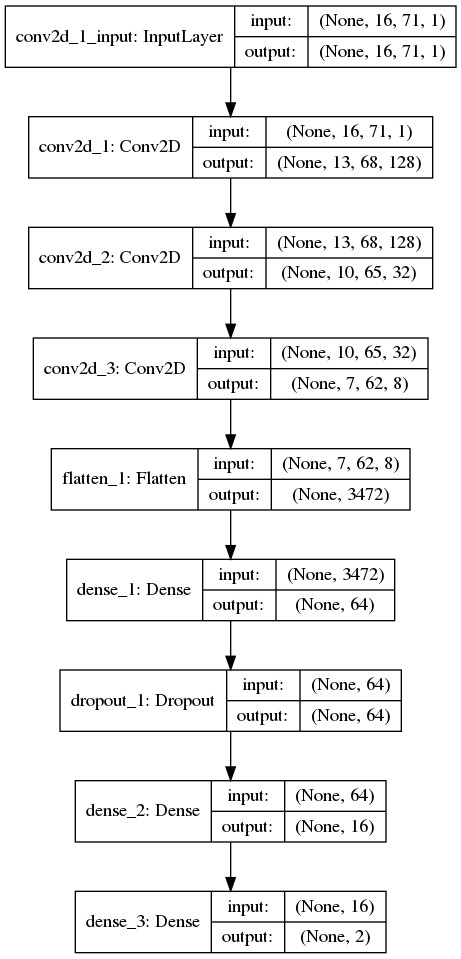
\includegraphics[scale=0.63]{section3/model.jpg}
	\caption{
نحوه‌ی چینش لایه‌های شبکه عصبی تشخیص صفرهای احتمالی}
	\label{CNNModel}
\end{figure}

بعد از آزمودن ساختارهای مختلف، شبکه‌ی عصبی عمیق مورد استفاده نهایی را همانند ساختار شکل
\ref{CNNModel}
مدل‌سازی کردیم. این شبکه دارای سه لایه کانولوشن دو بعدی و در امتداد آن سه لایه‌ی تماما متصل کانولوشن می‌باشد. لایه‌ی آخر دو خروجی برای پیش‌بینی تاثیر کاهنده و یا افزاینده دارد. لایه‌های‌ کانولوشن از فیلترهای مربعی با ابعاد ۴ و گام
\LTRfootnote{Stride}
۱ استفاده می‌کنند. همچنین هر لایه‌ی کانولوشن دارای یک تابع فعال‌سازی
\LTRfootnote{Activation Function}
\lr{Relu}
است. تعداد فیلترهای کانولوشن به ترتیب ۱۲۸، ۳۲ و ۸ می‌باشد. لایه‌های تماما متصل به‌ترتیب ۶۴، ۱۶ و ۲ گره دارند، دو لایه‌ی اول دارای فعال‌ساز
\lr{Relu}
بوده و لایه‌ی آخر با ۲ گره دارای فعال‌ساز 
\lr{Sigmoid}
می‌باشد. لایه‌های کانولوشن با استفاده از لایه‌ی هموارکننده
\LTRfootnote{Flatten}
به لایه‌های تماما متصل مرتبط می‌شود. وظیفه‌ی این لایه تغییر شکل مستطیلی دو بعدی به حالت برداری یک بعدی است. خروجی این لایه ورودی لایه‌ی اول تماما متصل می‌باشد. همچنین بین لایه‌های تماما متصل ۶۴ و ۱۶ گره‌ای از یک لایه‌ی
\lr{Dropout}
با مقدار دور ریخت ۰/۲ استفاده می‌شود.  مقدار ۰/۲ بیان می‌کند که شبکه در این لایه بصورت تصادفی بیست درصد ویژگی‌ها را درنظر نمی‌گیرد. این لایه بدین منظور استفاده می‌شود که از بیش‌برازش
\LTRfootnote{Overfit}
مدل جلوگیری کند و مدل را وادار می‌کند تا تعداد ویژگی‌های بیشتر و با اعتماد بالاتری را جهت پیش‌بینی استخراج و مورد استفاده قرار دهد و درصورت حذف تعدادی از آنها توان پیش‌بینی الگوریتم افت نکند و متکی به چند ویژگی خاص نباشد.
 
در بررسی‌ها مشاهده شد لایه‌های کانولوشن دوبعدی بهتر از نوع یک بعدی آنها کار می‌کنند، زیرا در این حالت فیلترها ‌می‌توانند شباهت‌های دارویی بیشتری را در هنگام پیمایش زیر نظرگرفته و این امکان وجود دارد ویژگی‌های قدرتمندتری را استخراج کنند. لذا بردارهای ویژگی ۱۱۳۶ بعدی به ماتریس‌هایی با ابعاد
$71 \times 16$
تغییر فرم داده می‌شوند. در شکل
\ref{paramNumber1}
تعداد وزن‌های قابل یادگیری هر لایه مشخص شده‌است. همچنین تعداد کل وزن‌ها که نشان دهنده‌ی میزان پیچیدگی کلی مدل است محاسبه شده‌است.

\begin{figure}[!h]
	\centering
	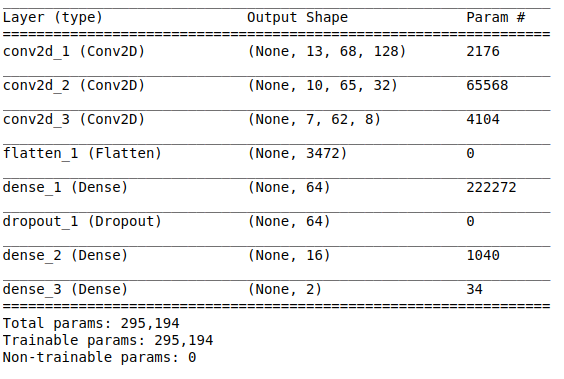
\includegraphics[width=\textwidth]{section3/modelparameters.png}
	\caption{
وزن‌های قابل یادگیری شبکه‌ی عصبی پیش‌بینی دوکلاسه}
	\label{paramNumber1}
\end{figure}

\newpage
در ساخت شبکه عصبی کانولوشن از تنظیمات زیر استفاده می‌شود:

۱) برای پیاده‌سازی شبکه عصبی از بسته‌های
\lr{Tensorflow}\cite{TENSORFLOW114}
(نسخه‌ی ۱.۱۴.۰) و
\lr{KERAS}\cite{KERAS2020}
(نسخه‌ی ۲.۲.۵) استفاده شد.

۲) از تابع بهینه‌سازی
\lr{ADAM}
استفاده شد.
 
۳) تابع خطا
\lr{Categorical-cross entropy}
در نظر گرفته شد.

۴) تعداد ایپوک
\LTRfootnote{Epoch}
ها ۵ در نظر گرفته شد. 

۵) نرخ یادگیری
\LTRfootnote{Lerning Rate}
۰/۰۰۰۰۱ استفاده شد.

درنظر داشته‌ باشید فراپارامترهای
\LTRfootnote{Hyperparameter}
این شبکه بهینه نشده ‌است و پارامترهای مشخص ‌شده لزوما در بهترین حالت خود نیستند. برای عدم بهینه‌سازی فراپارامترها دو دلیل وجود دارد:

۱) اجتناب از بیش‌برازش مدل
\LTRfootnote{Overfiting}:
در صورت تغییر فراپارامترها به بهترین مقادیر، انتظار می‌رود، مدل نتایج بهتری روی داده‌ی حاضر بگیرد، اما تضمینی وجود ندارد ویژگی‌های استخراج شده توسط مدل، معنی‌دار بوده و در صورت استفاده از مدل بر روی داروهای جدید به‌خوبی عمل کند. در این صورت اصطلاحا مدل بیش‌برازش شده و نکته‌ی منفی برای مدل خواهد بود. 

۲) حفظ استواری
\LTRfootnote{Robust}:
فراپارامترهای بهینه برای داده‌ی حاضر نتایج بهتری می‌دهند اما ممکن است در آینده از شباهت‌های دارویی متفاوتی استفاده شود یا داده‌های جدیدی جمع‌آوری شود و نتایج حاضر تکرار نشود. در این صورت مدل قوت و مستحکمی خود را از دست داده و مقبولیتی در جامعه‌ی داروسازی و داروشناسی نخواهد داشت.
 
 در نهایت نتایج مدل پیشنهادی را در روال اعتبارسنجی 10برابری از سه دیدگاه بررسی می کنیم:
 
 ۱) دقت مدل: مدل در روال اعتبارسنجی 10برابری برای تشخیص برهم‌کنش‌های کاهنده
$AUC=0/97$
و
$AUPR=0/93$ 
بدست آمد و برای تشخیص برهم‌کنش‌های افزاینده
$AUC=0/97$
و
$AUPR=0/99$
بدست آمد. این نتایج حاکی از دقت و توان تشخیص بالای مدل می‌باشد.
 
 ۲) واریانس نتایج: بازه‌ی اطمینان برای مقادیر گزارش‌شده با ضریب اطمینان بالای ۹۵ درصد باریک و نزدیک به‌هم بوده است. به شکلی که از چهار مقدار از سه مقدار گزارش شده کمتر از ۰/۰۰۲ بوده و  فقط برای تشخیص کاهنده مقدار 
\lr{AUPR}
 در بازه‌ی به اضافه و منهای ۰/۰۰۵ بوده‌است. با توجه به مقدار کم واریانس بدست آمده از مدل کاملا مشخص است که مدل ارایه شده استوار می‌باشد.
 

۳) توانایی تفکیک‌پذیری مدل: با رسم نمودار توزیع احتمالی خروجی ماشین مطابق شکل 
\ref{DDIProbHist}
 مشخص است که مقادیر 1 و 1- به‌خوبی از هم جدا شده‌اند و توزیع احتمال کاهنده و افزاینده اشترک کمی دارند. 


\begin{figure}[!h]
	\centering
	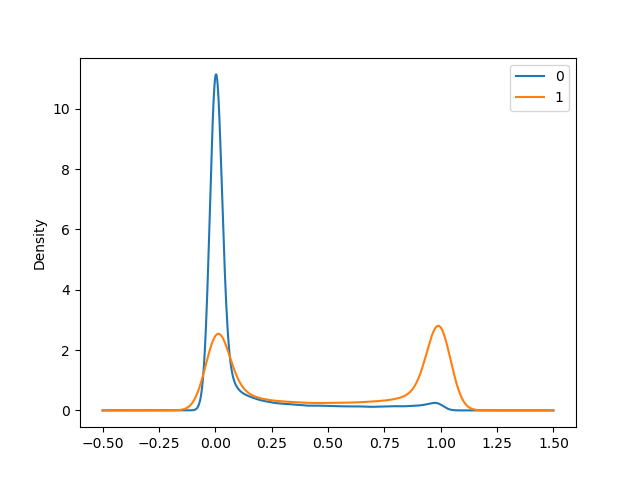
\includegraphics[scale=0.9]{section3/densityDegEnh.png}
	\caption{
نمودار توزیع چگالی احتمال کاهنده و افزاینده
}
در این شکل ۰ همان  برچسب ۱+ بوده و ۱ همان ۱- است.
	\label{DDIProbHist}
\end{figure}

شبه کد 
\ref{modelSelectionSuducode}
روند انتخاب مدل را مرحله به مرحله نشان می‌دهد.

\renewcommand{\algorithmicrequire}{\textbf{ورودی:}}
\renewcommand{\algorithmicensure}{\textbf{خروجی:}}
\begin{algorithm}[!h]
\caption{شبه کد انتخاب مدل}
\label{modelSelectionSuducode}
\begin{algorithmic}[1]
\REQUIRE 
ویژگی‌های جفت داروهای 1+ و 1-
\ENSURE 
مدل تشخیص دهنده 1+ و 1-
\vskip.5\baselineskip\hrule height 0.4pt\vskip.5\baselineskip

\STATE 
اعتبارسنجی متقابل 10 برابری را روی ویژگی‌های جفت داروهای 1+ و 1- اعمال کن.

\STATE 
مدل مناسب را انتخاب کن.

\STATE 
نتایج مدل را در روال اعتبارسنجی متقابل 10 برابری بررسی کن.

\STATE 
درصورت ارضای شرط ۳ مدل انتخابی را برگردان درغیراینصورت به مرحله ۲ بازگرد.

\end{algorithmic}
\end{algorithm}


\subsection{تشخیص جفت داروهای بدون برهم‌کنش احتمالی}

در مرحله‌ی قبل مدلی با دقت بالا، قوی و مستحکم ارائه شد که می‌توانست تاثیرات افزینده و کاهنده جفت داروها را به‌خوبی مدل کرده و تشخیص دهد. لذا این مدل به شرح زیر توانایی تشخیص غیربرهم‌کنش‌ها (صفرهای واقعی) را دارد. اگر با احتمال کمی جفت دارویی نامزد برهم‌کنش باشند، آنگاه آن جفت دارو، به احتمال زیاد، صفرهای واقعی هستند.

با توجه به این فرض، از مدل برای انجام پیش‌بینی روی کلیه‌ی جفت داروهای ناشناخته (صفرها) استفاده ‌شد. جفت داروهای ناشناخته شامل ۲۷۰۰۰۰ جفت دارو می‌باشد. در خروجی مدل، جفت داروهایی که با احتمال کمتر از ۰/۴ افزاینده و با احتمال کمتر از ۰/۴ کاهنده بودند را به  عنوان جفت داروهای بدون برهم‌کنش درنظر می‌گیریم. از بین داده‌هایی با برچسب ناشناخته حدود ۶۵۰۰۰ جفت دارو شرایط مذکور را داشتند. این دسته از جفت داروها نامزد عدم برهم‌کنش هستند. با توجه به دقت بالای مدل، واریانس کم نتایج و توانایی تفکیک‌پذیری بالای مدل، جفت‌های مذکور را به عنوان جفت داروهای فاقد برهم‌کنش در نظر می‌گیریم.

\subsection{آموزش مدل روی برهم‌کنش‌های شناخته‌شده و ناشناخته}

در این بخش از داده‌های شناخته شده و نامزدهای بالقوه برای عدم برهم‌کنش در جهت تشکیل مجموعه داده استفاده می‌شود. در این نگارش از این پس، جفت داروهای نامزد عدم برهم‌کنش را با عبارت صفر واقعی جایگزین کرده و به‌کار می‌بریم. همچنین برای مدل نهایی نیز از مدل توصیه‌گر ارائه‌شده در بخش
\ref{selected_model}
استفاده می‌شود. در ادامه روند کار به‌شکل مبسوط آمده است.

\subsubsection{روند اعتبارسنجی نتایج مدل پیش‌بینی برهم‌کنش داروها}
ابتدا سطرهایی از ماتریس
\lr{B}
که شامل برهم‌کنش‌‌‌های مثبت یک و منفی یک هستند مطابق روند مشروح در بخش
\ref{Model_selection_CV}
جدا شده و در 10 دسته قرار می‌گیرند. سپس به‌صورت تصادفی از میان ۶۵۰۰۰ جفت داروی نامزد بدون برهم‌کنش، ۳۰۰۰۰ جفت دارو انتخاب شد. در جفت داروی انتخابی، حتما باید خود جفت و دوگان آن نامزد بدون برهم‌کنش باشند. این گروه از صفرها به‌صورت تصادفی به ۱۰ دسته تقسیم می‌شوند. به‌گونه‌ای که دسته‌ی هر جفت دارو و دوگان یکسان باشد. سپس ۱۰ دسته‌ی صفرها با ۱۰ دسته‌ی از قبل آماده‌ی ۱+ و ۱- ها ادغام می‌شوند. 
 
حال مجموعه داده‌ای شامل تقریبا ۷۲۷۰۲ جفت دارو به دسته‌ی نسبتا برابر تقسیم شده و آماده‌ی استفاده برای روند آموزش و ارزیابی مدل نهایی توصیه‌گر می‌باشد.

\subsubsection{مدل نهایی پیش‌بینی برهم‌کنش داروها}

\begin{figure}
	\centering
	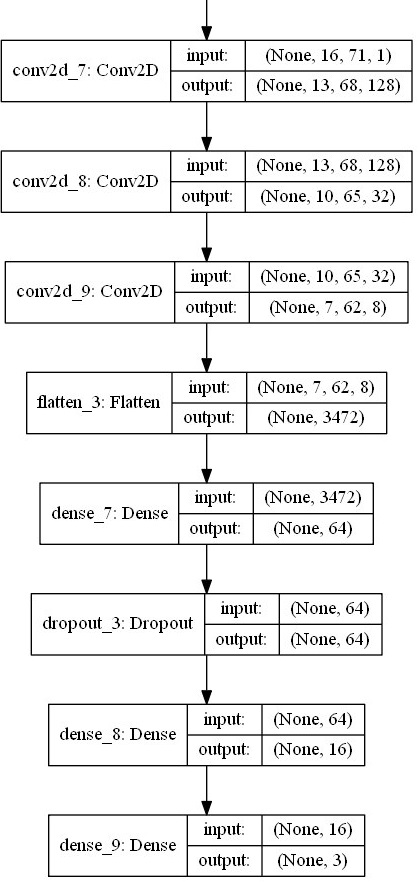
\includegraphics[scale=0.66]{section3/Triple_model.jpg}
	\caption{
چیدمان لایه‌های شبکه عصبی
\lr{SNF-CNN}
پیش‌بینی سه‌کلاسه برهم‌کنش
}
عدم برهم‌کنش (۰)، برهم‌کنش کاهنده (۱-) و برهم‌کنش افزاینده (۱+)
	\label{Triple_model}
\end{figure}
در قسمت قبل طریقه‌ی آماده‌سازی داده برای روال اعتبارسنجی مدل شرح داده‌شد. در این مرحله مدل نهایی ارائه می‌شود. مدل نهایی تقریبا همان مدل بیان شده در بخش 
\ref{selected_model}
است. یعنی شبکه سه لایه‌ی کانولوشن با تعداد فیلترهای کانولوشن ۱۲۸، ۳۲ و ۸ دارد. سپس همانند قبل از لایه‌های کانولوشن سه لایه تماما متصل استفاده شد. با این تفاوت که تعداد گره‌ها از ۶۴، ۱۶ و ۲  به ترتیب به ۶۴، ۱۶ و ۳ گره در هر لایه تغییر کرد. مشخصا این مدل سه خروجی احتمالی برای سه حالت برهم‌کنش افزاینده، عدم برهم‌کنش و برهم‌کنش کاهنده می‌دهد. همچنین تعداد ایپوک‌ها ۹ درنظر گرفته‌شد. روند انتخاب ایپوک در بخش
\ref{K-fold CV}
شرح داده ‌شده ‌است. مدل شبکه‌ی عصبی عمیق جهت پیش‌بینی برهم‌کنش در شکل
\ref{Triple_model}
نشان داده ‌شده ‌است. در این مرحله از انتخاب مدل جدید خودداری شد، زیرا:

۱) توان این مدل برای تشخیص نسبتا دقیق برهم‌کنش افزاینده و کاهنده در آخر بخش
\ref{selected_model}
به اثبات رسیده ‌است.

۲) صفرهای واقعی استفاده شده در این بخش پیشنهادی هستند و توسط آزمایشگاه داروشناسی تایید نشده‌اند و تا زمان نگارش این نوشتار پایگاه جامعی برای موارد عدم برهم‌کنش به‌صورت عمومی منتشر نشده ‌است. لذا اگر روند انتخاب مدل مجددا انجام شود، ممکن است مدلی انتخاب و استفاده شود که از نظر کاربرد در دنیای واقعی معتبر نبوده و مورد قبول قرار نگیرد.

با توجه به دلایل بالا مدل توصیه‌گر صفرها، با تغییر تعداد خروجی‌ها از ۲ به ۳ و تغییر داده‌های ورودی برای پیش‌برهم‌کنش‌های دارویی به‌کار می‌رود. فرآیند کلی روش پیشنهادی
\lr{SNF-CNN}
در قالب شبه کد 
\ref{SNFCNNSuducode}
ارائه شده است که شامل مراحل آماده‌سازی، انتخاب مدل، تشخیص صفر واقعی و ارائه‌ی توصیه‌گر جامع می‌باشد.

\renewcommand{\algorithmicrequire}{\textbf{ورودی:}}
\renewcommand{\algorithmicensure}{\textbf{خروجی:}}
\begin{algorithm}
\caption{
شبه کد روال کلی الگوریتم 
\lr{SNF-CNN}}
\label{SNFCNNSuducode}
\begin{algorithmic}[1]
\REQUIRE 
ویژگی‌های جفت داروها (1+، 1- و ۰های واقعی)
\ENSURE 
مدل تشخیص دهنده‌ی نوع برهم‌کنش و عدم‌برهم‌کنش (1+، 1- و ۰)
\vskip.5\baselineskip\hrule height 0.4pt\vskip.5\baselineskip

\STATE 
ماتریس‌های شباهت دارویی را با استفاده از روش کسینوس محاسبه کن.

\STATE 
ماتریس‌های شباهت دارویی را با استفاده از روش ترکیب شباهت شبکه‌ای ادغام کن.

\STATE 
ماتریس ورودی مدل را تشکیل بده.

\STATE 
مدل مناسب برهم‌کنش‌های شناخته شده را انتخاب کن و آموزش بده.

\STATE
صفرهای احتمالی را با استفاده از مرحله ۴ پیش‌بینی کن.
\STATE
مدل مناسب برهم‌کنش‌های شناخته شده و صفرهای مرحله ۵ را انتخاب کن و آموزش بده.
\STATE
روی جفت داروهای ناشناخته پیش‌بینی انجام بده.
\end{algorithmic}
\end{algorithm}


\section*{خلاصه‌ی فصل سوم و نگاهی به فصل چهار}
در این فصل روندی جامع برای آماده‌سازی داده ارائه ‌شد که می‌تواند بر روی ویژگی‌های مختلف اعمال شود و به انواع ماشین‌های یادگیرنده ورودی داده ‌شود. سپس مدل توصیه‌گری ارائه شد که نه تنها توانایی تشخیص نوع برهم‌کنش (افزاینده و کاهنده) را دارد بلکه می‌تواند جفت داروهایی را که به احتمال قوی باهم برهم‌کنش ندارند را نیز تشخیص دهد. روش ارائه شده به نام 
\lr{SNF-CNN}
نام‌گذاری شد. مدل توصیه‌گر سه‌کلاسه جامع در روند اعتبارسنجی آموزش و ارزیابی شد که نتایج آن در فصل چهار گزارش می‌شود. سپس برای اعتبارسنجی داروشناسی مدل با تمام جفت داروهای شناخته‌شده و صفرهای واقعی آموزش داده شد و روی تمام صفرها پیش‌بینی انجام شد و نتایج پیش‌بینی در پایگاه‌داده‌ی دارویی جست‌وجو شد که نتیجه اعتبارسنجی داروشناسی را نیز در فصل چهار ذکر شده و بررسی می‌شود.!
 قرار دهید.
\section{از کجا شروع کنم؟}
قبل از هر چیز، بدیهی است که باید یک توزیع تِک مناسب مانند 
\verb!Live TeX!
و یک ویرایش‌گر تِک مانند
\verb!Texmaker!
را روی سیستم خود نصب کنید.  ویرایش‌گر بهینه شده \verb!Texmaker! را می‌توانید از 
 \href{http://www.parsilatex.com}{سایت پارسی‌لاتک}%
\LTRfootnote{http://www.parsilatex.com}
 و\verb!Live TeX!  را هم می‌توانید از 
 \href{http://www.tug.org/texlive}{سایت رسمی آن}%
\LTRfootnote{http://www.tug.org/texlive}
 دانلود کنید.
 
در مرحله بعد، سعی کنید که  یک پشتیبان از پوشه 
\verb!SBU_thesis!
 بگیرید و آن را در یک جایی از هارد سیستم خود ذخیره کنید تا در صورت خراب کردن فایل‌هایی که در حال حاضر، با آن‌ها کار می‌کنید، همه چیز را از 
 دست ندهید.
 
 حال اگر نوشتن \پ اولین تجربه شما از کار با لاتک است، توصیه می‌شود که یک‌بار به طور سرسری، کتاب «%
\href{http://www.tug.ctan.org/tex-archive/info/lshort/persian/lshort.pdf}{مقدمه‌ای نه چندان کوتاه بر
\lr{\LaTeXe}}\LTRfootnote{http://www.tug.ctan.org/tex-archive/info/lshort/persian/lshort.pdf}»
   ترجمه دکتر مهدی امیدعلی، عضو هیات علمی دانشگاه شاهد را مطالعه کنید. این کتاب، کتاب بسیار کاملی است که خیلی از نیازهای شما در ارتباط با حروف‌چینی را برطرف می‌کند.
 
 
بعد از موارد گفته شده، فایل 
\verb!main.tex!
و
\verb!fa_title!
را باز کنید و مشخصات پایان‌نامه خود مثل نام، نام خانوادگی، عنوان پایان‌نامه و ... را جایگزین مشخصات موجود در فایل
\verb!fa_title!
 کنید. دقت داشته باشید که نیازی نیست 
نگران چینش این مشخصات در فایل پی‌دی‌اف خروجی باشید. فایل 
\verb!SBU.cls!
همه این کارها را به طور خودکار برای شما انجام می‌دهد. در ضمن، موقع تغییر دادن دستورهای داخل فایل
\verb!fa_title!
 کاملاً دقت کنید. این دستورها، خیلی حساس هستند و ممکن است با یک تغییر کوچک، موقع اجرا، خطا بگیرید. برای دیدن خروجی کار، فایل 
\verb!fa_title!
 را 
\verb!Save!، 
(نه 
\verb!As Save!)
کنید و بعد به فایل 
\verb!main.tex!
برگشته و آن را اجرا کنید. حال اگر می‌خواهید مشخصات انگلیسی \پ را هم عوض کنید، فایل 
\verb!en_title!
را باز کنید و مشخصات داخل آن را تغییر دهید.%
\RTLfootnote{
برای نوشتن پروژه کارشناسی، نیازی به وارد کردن مشخصات انگلیسی پروژه نیست. بنابراین، این مشخصات، به طور خودکار،
نادیده گرفته می‌شود.
}
 در اینجا هم برای دیدن خروجی، باید این فایل را 
\verb!Save!
کرده و بعد به فایل 
\verb!main.tex!
برگشته و آن را اجرا کرد.

برای راحتی بیشتر، 
فایل 
\verb!SBU.cls!
طوری طراحی شده است که کافی است فقط  یک‌بار مشخصات \پ  را وارد کنید. هر جای دیگر که لازم به درج این مشخصات باشد، این مشخصات به طور خودکار درج می‌شود. با این حال، اگر مایل بودید، می‌توانید تنظیمات موجود را تغییر دهید. توجه داشته باشید که اگر کاربر مبتدی هستید و یا با ساختار فایل‌های  
\verb!cls!
 آشنایی ندارید، به هیچ وجه به این فایل، یعنی فایل 
\verb!SBU.cls!
دست نزنید.

نکته دیگری که باید به آن توجه کنید این است که در فایل 
\verb!SBU.cls!،
سه گزینه به نام‌های
\verb!bsc!،
\verb!msc!
و
\verb!phd!
برای تایپ پروژه، پایان‌نامه و رساله،
طراحی شده است. بنابراین اگر قصد تایپ پروژه کارشناسی، پایان‌نامه یا رساله را دارید، 
 در فایل 
\verb!main.tex!
باید به ترتیب از گزینه‌های
\verb!bsc!،
\verb!msc!
و
\verb!phd!
استفاده کنید. با انتخاب هر کدام از این گزینه‌ها، تنظیمات مربوط به آنها به طور خودکار، اعمل می‌شود.
\section{مطالب \پ را چطور بنویسم؟}
\subsection{نوشتن فصل‌ها}
همان‌طور که در بخش \ref{sec2} گفته شد، برای جلوگیری از شلوغی و سردرگمی، قسمت‌های مختلف \پ از جمله فصل‌ها، در فایل‌های جداگانه‌ای قرار داده شده‌اند. 
بنابراین، اگر می‌خواهید مثلاً مطالب فصل ۱ را تایپ کنید، باید فایل‌های 
\verb!main.tex!
و
\verb!chapter1!
را باز کنید و محتویات داخل فایل 
\verb!chapter1!
را پاک کرده و مطالب خود را تایپ کنید. توجه کنید که همان‌طور که قبلاً هم گفته شد، تنها فایل قابل اجرا، فایل 
\verb!main.tex!
است. لذا برای دیدن حاصل (خروجی) فایل خود، باید فایل  
\verb!chapter1!
را 
\verb!Save!
کرده و سپس فایل 
\verb!main.tex!
را اجرا کنید. یک نکته بدیهی که در اینجا وجود دارد، این است که لازم نیست که فصل‌های \پ را به ترتیب تایپ کنید. می‌توانید ابتدا مطالب فصل ۳ را تایپ کنید و سپس مطالب فصل ۱ را تایپ کنید. 

نکته بسیار مهمی که در اینجا باید گفته شود این است که سیستم \lr{\TeX}، محتویات یک فایل تِک را به ترتیب پردازش می‌کند. به عنوان مثال، اگه فایلی، دارای ۴ خط دستور باشد، ابتدا خط ۱، بعد خط ۲، بعد خط ۳ و در آخر، خط ۴ پردازش می‌شود. بنابراین، اگر مثلاً مشغول تایپ مطالب فصل ۳ هستید، بهتر است
که دو دستور 
\verb!% !TeX root=main.tex

\chapter{مقدمه}
\pagenumbering{arabic}



در این بخش سعی می‌شود مفاهیم و تعاریف اولیه‌ی مورد نیاز برای ورود به مسئله‌ی اصلی به‌صورت مختصر تبیین گردد، سپس به تعریف مسئله می‌پردازیم.

\section{دارو}
در دانش پزشکی به هر ماده‌ای که برای درمان، تسکین علائم، تشخیص بیماری یا پیش‌گیری از آن به‌کار رود و بر ساختار یا کارکرد ارگانیسم زنده اثر گذارد و پس از ورود به بدن عملکرد بدن را تصحیح کند، دارو 
\LTRfootnote{Drug}
گفته می‌شود. در تعریفی دیگر دارو به ماده‌ای گفته می‌شود که با اثر بر گیرنده‌ای خاص در داخل، خارج یا دیواره‌ی سلول باعث شروع یا مهار عملکردی خاص ‌گردد و قدرت اثر دارو با میزان و تعداد این برهم‌کنش نسبت مستقیم دارد. البته داروهایی که  اثر موضعی دارند مانند آنتی اسیدها و ضدعفونی کننده‌های موضعی و مواد حاجب در این تعریف نمی‌گنجند 
\cite{Basic2018}.
امروزه اطلاعات دارو‌ها به طور گسترده در پایگاه‌داده‌های دارو قابل دسترسی می‌باشد که به تعدادی از مهم‌ترین آن‌ها در بخش
\ref{data base} 
اشاره می‌کنیم.
 
\section{داروشناسی}
داروشناسی
\LTRfootnote{Pharmacology} 
دانش بررسی واکنش مواد شیمیایی در سیستم‌های زیستی است. داروشناسی پزشکی
\LTRfootnote{Medical Pharmacology}
بخشی از داروشناسی که در ارتباط با استفاده از مواد شیمیایی در پیشگیری، تشخیص و درمان بیماری، به ویژه در انسان است. دو حوزه اصلی داروشناسی، فارماکودینامیک 
\LTRfootnote{Pharmacodynamic}
و فارماکوکینتیک
\LTRfootnote{Pharmacokinetic} 
هستند. به‌طور خلاصه فارماکودینامیک مطالعه‌ی اثرات داروها بر بدن و فارماکوکینتیک، اثر و رفتار بدن برروی داروهاست. به‌عبارت دیگر فارماکودینامیک به مبحث واکنش‌های دارو در مواجهه با گیرنده‌های زیستی و فارماکوکینتیک به بحث و تعریف جذب، توزیع، متابولیسم و دفع دارو در سیستم‌های زیستی می‌پردازد
\cite{katzung2019katzung}.
داروشناسی و داروسازی
\LTRfootnote{Pharmacy} 
دو واژه جدا از هم هستند که گاهی به ‌اشتباه به‌جای هم به‌کار می‌روند. داروشناسی نوع رفتار دارو و سیستم‌ زیستی (بدن) است ولی داروسازی در رابطه با مواد اولیه، آماده‌سازی، توزیع و مقدار
\LTRfootnote{Dose}
مصرف داروهای بی‌خطر و موثر است.
\subsection{برهم‌کنش فارماکوکینتیک}

فارماکوکینتیک تأثیر سیستم‌های زیستی بر داروها را نشان می‌دهد. عمده‌ی فرآیندهای دخیل در فارماکوکینتیک جذب، توزیع، متابولیسم و دفع هستند. بیماری‌های مختلف می‌توانند پارامترهای استاندارد فارماکوکینتیک معمول را تغییر دهند. در صورت مشخص شدن پارامترهای فارماکوکینتیک بیمار، تنظیم مقدار مصرف دارو برای یک بیمار خاص قابل محاسبه است
\cite{katzung2019katzung}.
وقتی دو دارو با‌هم مصرف می‌شوند، روند جذب، توزیع، متابولیسم یا دفع یکی یا هر‌دوی آن‌ها ممکن‌ است با رفتار مورد انتظار آن‌ها در حالتی که دارو به تنهایی مصرف می‌شود، متفاوت باشد. چنین تفاوت‌هایی را ناشی از برهم‌کنش‌های فارماکوکینتیک می‌دانیم که عبارتند‌ از:
\par
\subsubsection*{برهم‌کنش بر اساس جذب: }
این امکان وجود دارد که فرآیند جذب
\LTRfootnote{Absorption}
دارو (از دیواره‌ی روده) درصورتی‌که با داروی دیگری ترکیب شود، کاهش یا افزایش یابد. در فرآیند جذب از دیواره‌ی روده، برخی از داروهای تنگ‌کننده ‌عروق، به محض استفاده (ورود به بدن) با عملکرد موقتی در موضع و با محدودکردن اندازه ‌رگ‌ها باعث کند شدن جذب دیگر داروها می‌شوند. گاهی پزشکان از این پدیده بهره‌ می‌گیرند، برای مثال برخی بی‌حس‌کننده‌های موضعی را با داروهای آلفا۱-آدرنرژیک (اپی‌نفرین، نوراپی‌نفرین، سینفرین) که تنگ‌کننده عروق هستند، برای کندکردن جذب و تداوم اثر دارو در موضع مورد نیاز، به‌کار می‌برند
\citep{Rescigno2003}.

\par
\subsubsection*{برهم‌کنش بر‌اساس توزیع: }
توزیع
\LTRfootnote{Distribution}
دارو ممکن است تحت تاثیر داروهایی که دارای اثر رقابتی بر جایگاه اتصال پروتین‌های پلاسما می‌باشند قرار گیرد. به‌طور مثال داروهای آنتی‌باکتریال سولفوناميدی قابليت جابجايی داروهايی نظير متوتروکسات، فنی‌توئين، سولفونيل اوره‌ها و وارفارين از آلبومين پلاسما را دارند. یک دارو با ایجاد تغییراتی در محیط فیزیکی و در محیط  توزیع داروی دیگر، باعث تغییر انتشار داروی دوم می‌شود. برای مثال ديورتيک‌ها می‌توانند از طريق کاهش آب کلی بدن، ميزان انتشار آمينوگليکوزيدها را کاهش دهند و باعث تشديد سميت دارويی آمينوگليکوزيدها و ليتيوم بدليل افزايش غلظت پلاسمايی آنان شوند.

\par
\subsubsection*{برهم‌کنش بر اساس متابولیسم:‌ }
این نوع برهم‌کنش‌ها به‌خوبی اثبات‌ شده‌اند و از اهمیت بالای بالینی برخوردارند. متابولیسم
\LTRfootnote{Metabolism}
اکثر دارو‌ها در کبد توسط آنزیم سیتوکروم
\lr{P450}
صورت می‌گیرد. متابولیسم یک دارو در صورت تجویز همزمان با داروهایی که اثر القاکنندگی بر این آنزیم‌ها دارند، افزایش می‌یابد و  متابولیسم یک دارو در صورت تجویز همزمان با داروهایی که اثر مهارکنندگی بر این آنزیم‌ها دارند، کاهش می‌یابد. 

\par
\subsubsection*{برهم‌کنش بر‌اساس دفع: }
دفع
\LTRfootnote{Elimination}
بسیاری از داروها از طریق ادرار و سیستم کلیوی صورت می‌گیرد. برای مثال دفع یک دارو در صورت استفاده همزمان با داروهای کاهنده جريان خون کليوی، کاهش می‌یابد و یا مصرف هم‌زمان یک دارو با داروهای تغيير‌دهنده‌ی
\lr{PH}
ادرار، ميزان يونيزاسيون آن دارو را کاهش‌ می‌دهد.


\subsection{برهم‌کنش فارماکوداینامیک}
ممکن‌ است استفاده هم‌زمان دو دارو منجر به افزایش تاثیرات هر یک از آن‌ها شود یا برعکس ممکن‌ است اثرات یکدیگر را سرکوب کنند. به‌چنین تاثیرات افزایشی یا کاهشی داروها بر روی یکدیگر، برهم‌کنش‌های فارماکوداینامیک می‌گوییم که عبارتند از:

\subsubsection*{برهم‌کنش بر‌اساس اثر آنتاگونیسم: }

ساده‌ترین نوع برهم‌کنش دارویی است که اغلب قابل پیش‌بینی است. گاهی اوقات جذب یک دارو مانع جذب بعضی داروهای دیگر می‌گردد، این پدیده را آنتاگونیسم یا رقابت‌کنندگی\LTRfootnote{Antagonism}گویند\cite{kenakin1997pharmacologic}.
برای مثال دارو‌های ضد التهابی غیراستروئیدی
\lr{NSAIDs}
اثر ضد فشار داروی مهارکننده‌ی
\lr{ACEIs}
را از طریق کاهش دفع سديم، کم می‌کنند.

\subsubsection*{برهم‌کنش بر‌اساس اثر سینرژیسم: }
گاهی جذب یک دارو باعث تشدید و افزایش شدت جذب داروی دیگر می گردد، به این پدیده سینرژیسم یا تشدیدکنندگی\LTRfootnote{Synergnism}گویند\cite{chou2006theoretical}.
جمع‌جبری اثرات دو دارو، ممکن‌ است بر يک گيرنده‌ی خاص عمل نمايند. اگر مجموع اثرات دو دارو با هم از جمع اثر هر دارو  به‌تنهايی بيشتر باشد تداخل فوق سینرژیسم یا تشدید‌کنندگی می‌باشد.                

\section{پایگاه داده‌های دارو
\label{data base}}
 
اطلاعات دارویی مورد نیاز برای حل مسائل مختلف مرتبط با دارو، در پایگاه داده‌های معروفی به شرح زیر موجود هستند. 
 
\begin{figure}[h!]
	\centering
	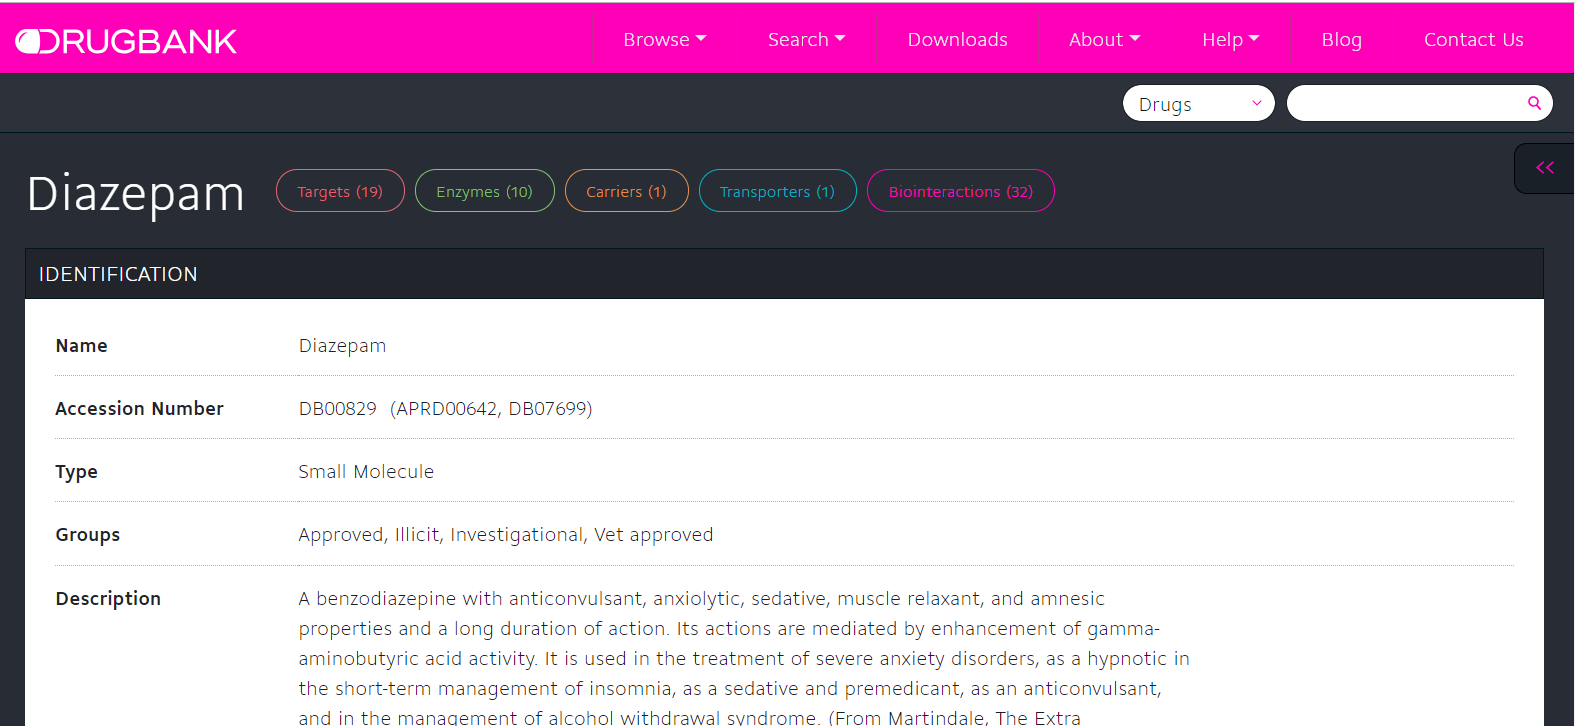
\includegraphics[scale=0.48]{section1/di.jpg}
	\caption{
قسمتی از نمایش اطلاعات داروی دیازپام در پایگاه داده‌ی
DrugBank}
	\label{fs1}
\end{figure}


\subsection{DrugBank}

\lr{DrugBank}
\cite{law2013drugbank,wishart2007drugbank,knox2010drugbank,wishart2006drugbank}:
یکی از منابع مهم تحقیقاتی بیوانفورماتیک می‌باشد که در آن اطلاعات دارو-هدف
\LTRfootnote{Drug-Target}،
آنزیم‌های دارو، انتقال‌ دهنده‌های دارو
‌\LTRfootnote{Drug Transporters}،
عوارض جانبی
\LTRfootnote{Side Effect}
دارو، برهم‌کنش‌های شناخته شده‌ی دارو با دیگر داروها و... موجود می‌باشد. درشکل
\ref{fs1} 
قسمتی از  اطلاعات داروی دیازپام
\LTRfootnote{Diazepam} 
نشان‌ داده‌ شده‌ است و در شکل 
\ref{fs2} 
قسمتی از اطلاعات برهم‌کنش داروی دیازپام با دیگر داروها نمایش داده شده‌ است. 

\begin{figure}[h!]
	\centering
	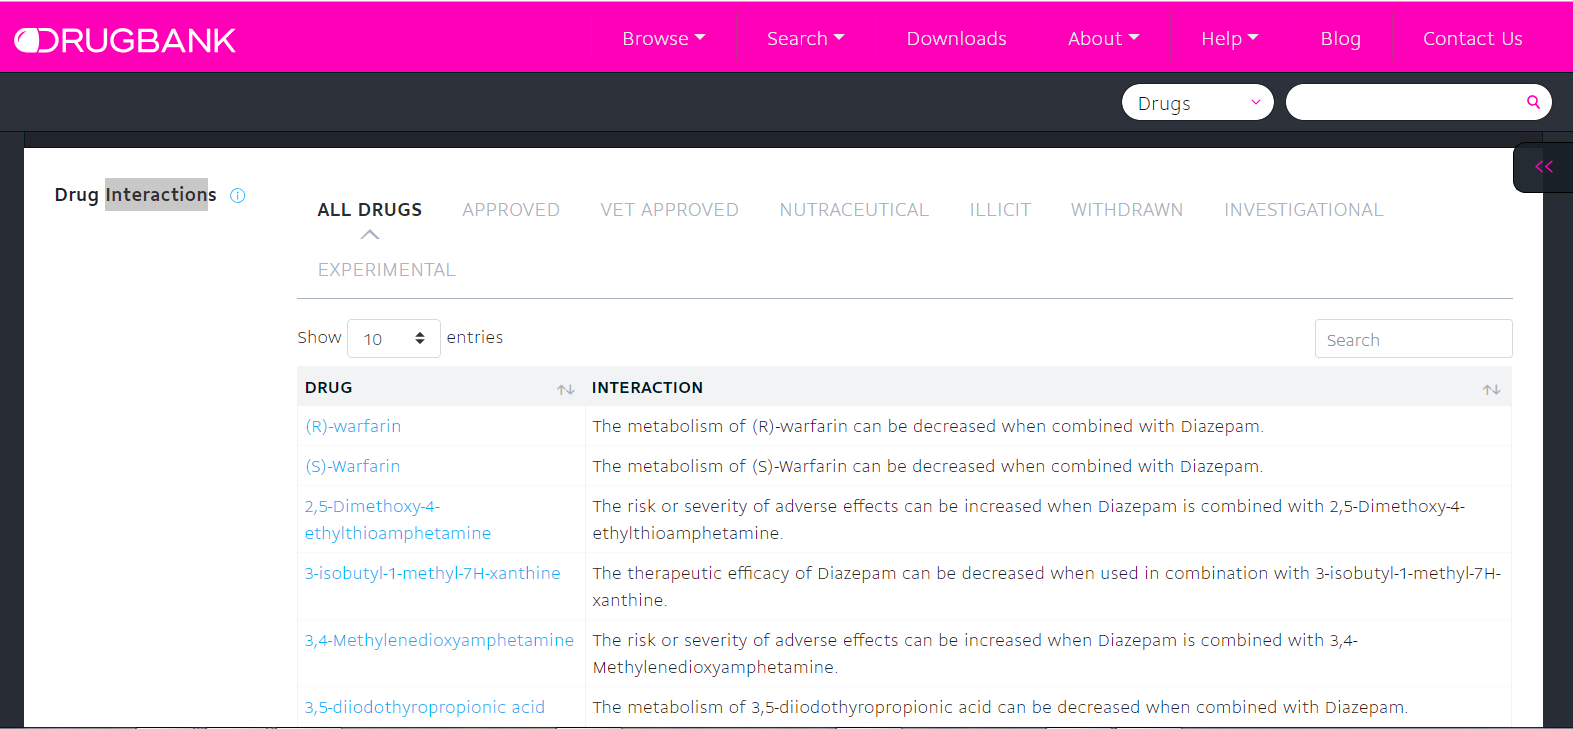
\includegraphics[scale=0.48]{section1/ddidi.png}
	\caption{
نمایش قسمتی از اطلاعات برهم‌کنش داروی دیازپام با دیگر داروها
	}
	\label{fs2}
\end{figure}

\subsection{KEGG}

\lr{KEGG}\LTRfootnote{Kyoto Encyclopedia of Genes \& Genomes}\cite{ogata1999kegg, kanehisa2000kegg}:
پایگاه داده‌ای مربوط به اطلاعات زیستی‌است که اولین بار توسط مینورور کانهیزا
\LTRfootnote{Minoru Kanehisa}
پروفسور موسسه‌ی تحقیقات شیمی در دانشگاه کیوتو در سال ۱۹۹۵ هم‌زمان با پروژه ژنوم درست شد. به منظور استفاده از تحلیل کامپیوتری برای تفسیر نتایج حاصل از پروژه ژنوم مینورور شروع به ساخت
\lr{KEGG Pathway}
کرد. در این پایگاه داده توسط دانش به‌دست آمده از آزمایش‌های مختلف، نقشه و مسیرهای متابولیکی ترسیم شده‌‌است و همچنین تعدادی از عملکرد‌های سلول‌ها و ارگانیزم‌ها به‌صورت جزئی به تصویر کشیده‌ شده‌‌است. هر نقشه شامل یکسری واکنش بین بیومولکول‌های مختلف می‌باشد که طوری طراحی شده‌است که از آن می‌شود اطلاعاتی در مورد ژن‌ها و پروتئین‌های دخیل در آن یافت. در این پایگاه‌داده می‌توان مسیرهای مختلف را با هم مقایسه و تحلیل کرد و به‌طور کلی از آن‌ها اطلاعات سودمندی استخراج کرد.
بر طبق نظر سازنده‌، 
\lr{KEGG} 
به صورت یک کامپیوتر ارائه دهنده‌ی سیستم‌های بیولوژیکی می‌باشد که دیاگرام‌ها و واحدهای متصل به هم ایجاد می‌کند. دیاگرام‌ها شامل ژن‌ها و عملکرد پروتئین‌های مرتبط، واکنش‌های بین مولکولی هستند. همچنین
\lr{KEGG} 
منبع مناسبی برای مسیرهای پروتئین 
\LTRfootnote{Protein Pathways}
 می‌باشد. در شکل 
\ref{fs3} 
صفحه‌ی اول این پایگاه داده که یک معرفی از آن می‌باشد نمایش داده شده است.

\begin{figure}[h!]
	\centering
	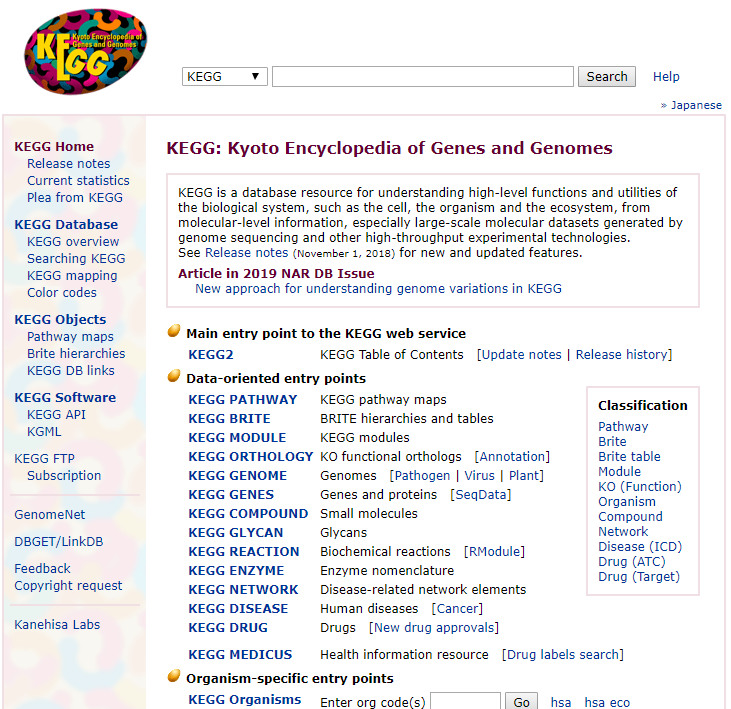
\includegraphics[scale=0.7]{section1/kegg1.PNG}
	\caption{ 
صفحه اول پایگاه داده KEGG}
	\label{fs3}
\end{figure}

\subsection{TWOSIDES}

\lr{TWOSIDES}\cite{Tatonetti2012}:
بانک اطلاعاتی عمومی حاوی عوارض‌جانبی ناشی از برهم‌کنش دارو–دارو  است. این بانک اطلاعاتی حاوی 868221 ارتباط بین 59220 جفت دارو و 1301 عوارض‌جانبی است. این ارتباطات فقط به مواردی محدود می شوند كه به‌طور واضح به‌هیچ یك از داروها اختصاص نیافته است (ارتباط‌های تحت پوشش
\lr{OFFSIDES}).
این پایگاه داده حاوی 3782910 ارتباط مهم دیگر است که، جفت داروها دارای نمره عوارض‌جانبی بالاتری هستند که با استفاده از نسبت گزارش متناسب 
\LTRfootnote{Proportional Reporting Ratio(PRR)}،
تعیین می‌شوند.

\subsection{FAERS}

\lr{FAERS}\LTRfootnote{FDA Adverse Event Reporting System} :
سیستم گزارش‌دهی رویدادهای ناخواسته‌ی سازمان غذا و دارو پایگاه داده‌ای، حاوی اطلاعات مربوط به عوارض‌جانبی ارسال شده به سازمان غذا و دارو\LTRfootnote{Food and Drug Adminstration(FDA)}است. این پایگاه داده، توسط
\lr{FDA}\LTRfootnote{http://www.fda.gov}،
به‌منظور پشتیبانی از برنامه‌ی نظارت بر ایمنی پس از بازاریابی برای داروها و محصولات بیولوژیکی درمانی طراحی شده است. داده‌های استخراج شده از 
\lr{FAERS}
 و 
\lr{TWOSIDES} 
مجموعه داده‌ای است که فقط شامل عوارض‌جانبی است که به دلیل ترکیب داروها ایجاد می شود 
\cite{Zhang2015}.

\subsection{SIDER}

\lr{{SIDER}}\cite{kuhn2015sider}:
در این پایگاه داده اطلاعات عوارض جانبی دارو‌ها و نشانگان دارو وجود‌ دارد. این پایگاه داده حاوی اطلاعاتی در مورد داروهای بازار و واکنش‌های دارویی نامطلوب آن‌ها است. با وجود این‌که
\lr{SIDER}
منبع مهمی از عوارض جانبی شناخته شده است، اما اطلاعات آن محدود است
\cite{Zhang2015}.
زیرا:

الف) آزمایشات بالینی بر روی جمعیت نسبتاً کمی از بیماران انجام می‌شود و فقط عوارض‌جانبی متداول با اطمینان بالا در لیست دارویی مشاهده می‌شوند.

ب) از طرفی عارضه‌ی‌جانبی مشاهده ‌شده در طول آزمایشات بالینی ممکن است اتفاقی باشد و در واقع توسط دارو ایجاد نشده باشد. 

لازم به ذکر است، عوارض‌جانبی‌ که از این پایگاه ‌داده استخراج شده ‌است 
\lr{Labele Side Effect}
نامیده می‌شود.

در شکل 
\ref{fs5} 
نمایی از صفحه‌ی اول پایگاه داده‌ی
\lr{SIDER}
مشاهده می‌شود که می‌توان براساس نام دارو یا عارضه‌جانبی در این پایگاه ‌داده جستجو نمود. 
\begin{figure}[h!]
	\centering
	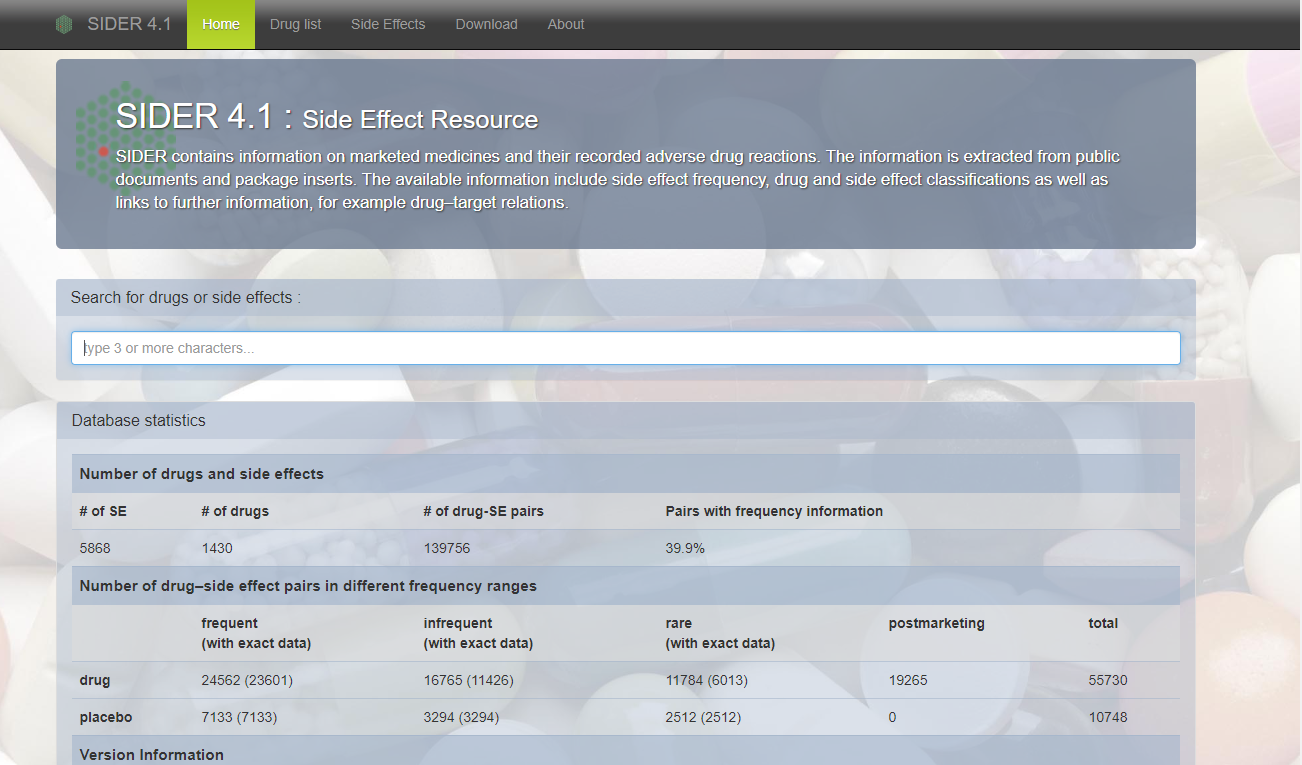
\includegraphics[scale=0.48]{section1/Sider1.png}
	\caption{ 
صفحه اول پایگاه داده SIDER}
	\label{fs5}
\end{figure}


\subsection{OFFSIDES}

مجموعه‌ای از عوارض‌جانبی داروها است که حاصل کاوش عوامل مخدوش کننده مانند مصرف داروهای همزمان، اطلاعات دموگرافیک بیمار و تاریخچه پزشکی بیمار از پایگاه‌داده‌ی 
\lr{FAERS} 
است. در این پایگاه‌داده 1332 دارو و 10093 عارضه‌جانبی وجود دارد. لازم به ذکر است، عوارض‌جانبی استخراج شده از 
\lr{OFFSIDES}
 با عنوان 
\lr{Off-Label Side Effect}
نامگذاری ‌می‌شود
\cite{Tatonetti2012}.

\subsection{PubChem}

پایگاه داده مربوط به مولکول‌های شیمیایی است که توسط موسسه ملی سلامت در ایالات متحده
\LTRfootnote{National Institutes of Health}
ایجاد شده است. این سامانه شامل مولکول‌های کوچکی است که کمتر از ۱۰۰۰ اتم یا ۱۰۰۰ پیوند شیمیایی دارند و اطلاعات ساختار شیمیایی
\LTRfootnote{Chemical Structure}
داروها را در بر دارد
\cite{Y. Wang2009}.

\section{ویژگی‌های داروها} 

\par
هر دارو می‌تواند به صورت یک بردار ویژگی دودویی، توسط معیار‌های مختلفی تعریف شود
\cite{cheng2014machine, zhang2017predicting}.
قبل از معرفی این ویژگی دو تعریف ارائه می‌شود که در درک بهتر عددی ویژگی‌ها کمک می‌کند.

\begin{definition}{اثر‌انگشت دارو}
  
اثر انگشت
\LTRfootnote{Drug Fingerprint}،
برداری از مقادیر باینری صفر و یک ویژگی‌های یک مولکول است. برای مثال اثر انگشت
\lr{MACCS key166}
نمونه‌ی‌ مشهوری با 166 ویژگی زیرساختار است که وجود یا عدم وجود یک زیرساختار را در این دارو مشخص می‌کند. وجود زیرساختارهایی با کم‌تر از سه اتم اکسیژن در ساختار شیمیایی دارو با یک کد می‌شود. همچنین عدم وجود زیر‌ساختار 
\lr{4mRing}
با صفر کد می‌شود که در شکل  
\ref{fs6}
به‌خوبی نمایش داده شده ‌است. به‌عنوان مثالی دیگر در اثر انگشت عوارض‌جانبی دارو، وجود یا عدم وجود هر عارضه‌ی جانبی مانند: سردرد، اسهال، حالت تهوع و... برای یک دارو به ترتیب با یک و صفر کد می‌شود.
  
\begin{figure}[!h]
	\centering
	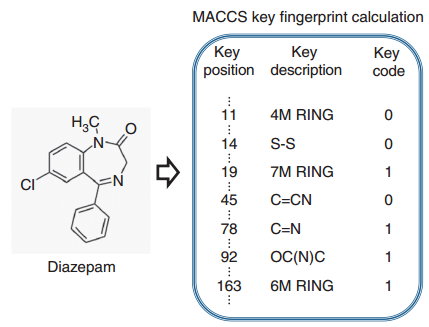
\includegraphics[scale=0.85]{section1/fing.png}
	\caption{نمایش نحوه ساخت اثر انگشت دارو}
	\label{fs6}
\end{figure} 

\end{definition}

\begin{definition}{خارج از برچسب}

برای توصیف داروی پزشکی به‌کار می‌رود. درصورتی که دارویی برای درمان بیماریی تجویز شود ولی برای درمان آن بیماری از طرف 
\LR{FDA}
تایید نشده باشد به آن نوع از استفاده، خارج از برچسب
\LTRfootnote{Off - Label}
می‌گویند. مثلا ممکن است دارویی برای معالجه کودک تایید شود اما از آن برای درمان بزرگسالان استفاده شود. نمونه‌ی دیگری از خارج از برچسب در بخش 
\ref{sideeffect}
معرفی می‌شود.
\end{definition}

\subsection{ساختار شیمیایی}

881 نوع زیرساختار مختلف تعریف شده است که یک دارو ممکن است آن‌ها را داشته یا نداشته باشد.  ساختار شیمیایی داروها در پایگاه داده‌های دارو نظیر 
\lr{DrugBank}
 یا 
\lr{PubChem}\cite{Y. Wang2009}
 در قالب فایل 
\lr{mol}،
\lr{smiles}
 و 
\lr{sdf}
 وجود دارند. در شکل
\ref{fs4} 
ساختار شیمیایی داروی دیازپام نشان‌داده شده ‌است.

\begin{figure}
	\centering
	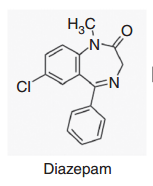
\includegraphics[scale=0.99]{section1/chem.png}
	\caption{	
	 ساختار شیمیایی داروی دیازپام }
	\label{fs4}
\end{figure}

\subsection{عوارض‌جانبی}
\label{sideeffect}

داروها می‌توانند عوارض‌جانبی ایجاد کنند. برخلاف تصور عموم، که عوارض‌جانبی دارو را فقط مختص مصرف خودسرانه‌ی دارو می‌دانند، باید دانست که عوارض‌جانبی بر اثر مصرف همه‌ی انواع داروها ایجاد می‌شوند؛ هم داروهایی که توسط پزشک تجویز شده‌اند و هم داروهایی که بدون نسخه تهیه می‌شوند. برای مثال، برخی آنتی‌بیوتیک‌ها مثل خانواده‌ی پنی‌سیلین‌ها، می‌توانند در افراد واکنش‌های حساسیتی ایجاد کنند. دانه‌های ریزپوستی
\LTRfootnote{Skin Rash}،
شایع‌ترین عارضه‌ی واکنش‌های حساسیتی به پنی‌سیلین‌ها و آنافیلاکسی مهم‌ترین یا خطرناک‌ترین عارضه‌ی ثانویه‌ی مصرف پنی‌سیلین‌ها به‌شمار می‌روند.
در این‌جا عوارض‌جانبی به دو دسته‌ی زیر تقسیم‌بندی می‌شوند:

عوارض جانبی برچسب‌دار
\LTRfootnote{Label Side Effect} 

عوارض جانبی خارج از برچسب
\LTRfootnote{Off-Label Side Effect}

\subsection{آنزیم‌}

بسیاری از داروها اثر خود را از طریق انجام واکنش با آنزیم‌ها
\LTRfootnote{Enzymes}
 اعمال می‌کنند. 
\lr{Cytochrome P450}
یک خانواده گسترده از آنزیم‌های هموپروتئینی است که در تمام موجودات زنده وجود دارد و ایزوآنزیم
\lr{CYP}
بیشتر متابولیسم داروها را انجام می‌دهد. همچنین فعال‌شدن بسیاری ترکیبات شیمیایی در درون بدن توسط همین ایزوآنزیم‌ها انجام می‌گیرد.
  
\subsection{منتقل کننده‌}

انتقال دارو یک موضوع حیاتی در پزشکی و درمان است. انتقال داروی کنترل‌شده، دسترسی به دارو را به واسطه جلوگیری از تجزیه در زمان نامناسب، افزایش دریافت دارو، حفظ غلظت دارو در طی درمان به واسطه کنترل سرعت آزادسازی دارو و کاهش عوارض جانبی از طریق هدفمندی دارو به جایگاه و سلول خاص را بهبود می‌بخشد. برای کاهش میزان تجزیه‌ی دارو، جلوگیری از عوارض جانبی مضر، افزایش دسترسی به دارو و تجمع دارو در ناحیه هدف، سیستم‌های متنوع انتقال و هدفمندی دارو در حال پیشرفت است. برای آزادسازی پیوسته‌ی دارو بایستی از پلیمرهایی استفاده کرد که دارو را با سرعتی قابل کنترل منتشر کنند یا با تجزیه‌ی پلیمر طی زمان آزاد شوند. در بین حامل‌های دارویی می‌توان پلیمرهای محلول، میکرو ذرات تشکیل شده از پلیمرهای طبیعی و سنتزی غیرمحلول و تجزیه‌پذیر، میکروکپسول‌ها، سلول‌ها، لیپوپروتئین‌ها، لیپوزوم‌ها و میسل‌ها را نام برد. حامل‌ها می‌توانند تجزیه پذیر، القایی (مثلا حساس به دما)، و حتی با تعبیه آنتی‌بادی خاص علیه ترکیبات ناحیه‌ی موردنظر هدفمند شوند.

\subsection{پروتیئن هدف}

ممکن است دارو به پروتئین‌های مختلفی بچسبد. در طراحی دارو به این نکته توجه می‌شود که از لحاظ هندسی دارو مکمل پروتئین هدف باشد تا بتواند به خوبی به آن متصل شود.

\subsection{نشانگان}

به بیماری‌هایی که دارو برای آنها تجویز می‌شود نشانگان
\LTRfootnote{Indication}
 گفته‌ می‌شود، ممکن‌ است یک دارو در درمان چند نوع بیماری موثر باشد.

\subsection{برهم‌کنش غذا - دارو}

برهم‌کنش غذا - دارو
\LTRfootnote{Food - Drug Interaction}
در اثر واکنش بین دارو و مواد خاص خوردنی یا نوشیدنی به وجود می‌آید. مثلاً آهن و کلسیم موجود در خوراکیها، مکمل‌های ویتامینی و داروهای ضد اسید معده، در معده به آنتی‌بیوتیک‌ها چسبیده و از جذب آنها به داخل خون جلوگیری می‌کنند. به‌عنوان یک مثال ساده‌، می‌توان ممنوعیت مصرف آنتی‌بیوتیک خوراکی همراه با شیر را ذکر کرد.

\subsection{ویژگی های سه بعدی }

ساختار شیمیای سه بعدی داروها
\LTRfootnote{3-D Drug Chemical Structure}
اطلاعاتی از نوع اتم‌ها و نحوه‌ی جای‌گیری آن‌ها در فضا ارائه می‌دهد. این ویژگی‌ها با استفاده از نرم‌افزار‌های خاصی اندازه‌گیری می‌شوند.



\par
\section{تعریف مسئله}
هنگامی که پزشک به‌طور همزمان چند دارو برای یک بیمار تجویز می‌کند، برهم‌کنش دارو–دارو  ممکن است عوارض‌جانبی جبران‌ناپذیری ایجاد کند، به‌طور مثال ممکن است تاثیرات داروها بر روی یکدیگر منجر به بیماری‌ها‌ی دیگر و یا حتی مرگ شود. این تاثیرات جانبی به‌طور خاص در افراد پیر و بیماران سرطانی که در روز تعداد زیادی دارو مصرف می‌کنند، چشم‌گیرتر است. عوارض‌جانبی یک دارو تا حد قابل قبولی در فاز توسعه دارو شناسایی می‌شود ولی عوارض‌جانبی حاصل از برهم‌کنش دارو–دارو  به دلیل دامنه گسترده مسئله به‌ندرت کشف می‌شود. چنین تاثیراتی عمدتا پس از تایید دارو و ورود دارو به بازار مصرف شناسایی می‌شوند که این خطری جدی برای سلامتی بیماران است. این مسئله از نظر اقتصادی نیز مهم ‌است زیرا پس از شناسایی برهم‌کنش مخرب یک دارو با داروی دیگر، ممکن‌ است آن دارو به طور کل از بازار جمع‌آوری شود. از طرفی به‌دلیل پرهزینه بودن روش‌های آزمایشگاهی، از مدل‌های پیش‌بینی برهم‌کنش دارو–دارو  استفاده می‌کنند. برای این مسئله تا‌کنون روش‌های متنوع محاسباتی، آماری، یادگیری‌ماشین و غیره ارائه شده‌است. در این پایان‌نامه روشی نوین برای حل این مسئله ارائه می‌دهیم.
 
\subsection{برچسب برهم‌کنش‌ها}  

به‌طور‌کلی به برهم‌کنش دارو–دارو  یکی از دو برچسب زیر را نسبت می‌دهند:

\textbf{برچسب مثبت}:
اگر وجود برهم‌کنش بین دو دارو با شواهد موجود ثابت شده‌ باشد و حداقل در یکی از پایگاه داده‌های دارو ثبت شده‌ باشد.

\textbf{برچسب منفی}:
برهم‌کنش دارو–داروهایی در این دسته قرار‌ می‌گیرند که تاکنون شناخته‌ نشده‌اند و در هیچ‌یک از پایگاه داده‌های مربوط به دارو ثبت نشده‌اند. در‌واقع با گذشت زمان ممکن‌ است شواهدی مبنی‌بر وجود برهم‌کنش بین دو دارو یافت شود و این برهم‌کنش برچسب مثبت بگیرد، اما تاکنون چنین اطلاعاتی در دست نیست.
\par
در این پایان‌نامه،به برهم‌کنش دارو–دارو  یکی از سه برچسب زیر را نسبت می‌دهیم:

\textbf{برچسب مثبت یک}:
اگر وجود برهم‌کنش بین دو دارو با شواهد موجود افزاینده باشد و حداقل در یکی از پایگاه داده‌های دارو ثبت شده‌ باشد.

\textbf{برچسب منفی یک}:
اگر وجود برهم‌کنش بین دو دارو با شواهد موجود کاهنده باشد و حداقل در یکی از پایگاه داده‌های دارو ثبت شده‌ باشد.

\textbf{برچسب صفر}:
اگر وجود برهم‌کنش بین دو دارو تاکنون شناخته نشده‌ باشد و در هیچ‌یک از پایگاه داده‌های دارو ثبت نشده‌ باشد.

\par 

\section{ساختار پایان‌نامه}
در ادامه‌ی این پایان‌نامه، ابتدا در فصل دو به بررسی پیشینه‌ی تحقیق و کار‌های انجام‌شده برروی داد‌ه‌های سه کلاسه از برهم کنش دارو - دارو می‌پردازیم. در مرحله‌ی بعد مفاهیم پیش نیاز برای ارائه روش پیشنهادی خود را معرفی می‌کنیم. این مفاهیم شامل دو بخش آماده‌سازی داده و رویکرد عمده‌ی انتخاب مدل می‌باشد.

در فصل سه، مجموعه‌داده‌ی به‌کار‌رفته را شرح خواهیم داد و روش پیشنهادی خود را با شرح مبسوط فرآیند کار برای حل مساله  مطرح خواهیم کرد. 

در فصل چهار به تحلیل و ارزیابی و بحث روی نتایج خواهیم پرداخت. در ادامه و در فصل پنج روش‌های پیشنهادی و کارهای آتی در جهت بهبود ارائه می‌شوند.

 
!
و
\verb!% !TeX root=main.tex
\chapter{بررسی تاریخچه‌، مفاهیم اولیه و الگوریتم‌های پیش‌بینی برهم‌کنش دارو-دارو}



\section{پیشینه تحقیق}
\label{intro}
هنگامی که دو یا چند دارو باهم مصرف می‌شوند، اثرات دارویی یا رفتارهای آن‌ها به‌طور غیرمنتظره‌ای تحت تاثیر یکدیگر قرار می‌گیرند
\cite{Wienkers2005}. 
این نوع تاثیرگذاری به‌عنوان برهم‌کنش دارو-دارو نامیده می‌شود که می‌تواند تاثیر دارویی را کاهش دهد، مسمویت غیرمنتظره را افزایش دهد یا بین داروهای تجویز شده عوارض‌جانبی ایجاد کند. با افزایش داروهای تایید شده، تعداد برهم‌کنش‌ دارو-داروهای ناشناخته به سرعت در حال افزایش است، به‌طوری‌که در بین داروهای کوچک مولکول تایید شده در 
\lr{Drug‌Bank}،
به‌طور متوسط از هر یکصد جفت دارو تقریبا حدود پانزده‌تای آن‌ها دارای برهم‌کنش دارو-دارو هستند
\cite{Law2014}. 
برهم‌کنش دارو-داروهای ناشناخته باعث می‌شود بیمارانی که با چندین دارو تحت درمان هستند، در وضعیت ناایمن قرار گیرند
\cite{Leape1995, Businaro2013,Karbownik2017,Mulroy2017}. 
همچنین درک برهم‌کنش دارو-دارو اولین قدم برای ترکیب داروهاست که به یکی از راهکارهای امیدوارکننده برای درمان بیماری‌های پیچیده تبدیل می‌شود
\cite{Zhao2011}. 
بنابراین، غربالگری و تجزیه‌ و‌ تحلیل برهم‌کنش دارو-داروها قبل از تجویز بالینی داروها، یک نیاز فوری است. با‌این‌حال، رویکردهای سنتی برای شناسایی برهم‌کنش دارو-دارو (به‌عنوان مثال، در آزمایش 
\lr{Cytochrome P450}\cite{Veith2009} 
یا برهم‌کنش مربوط به انتقال‌دهنده‌ی دارو
\cite{Huang2007}) 
با چالش‌هایی روبه‌رو است. از آن جمله می‌توان هزینه‌های بالا، مدت زمانی طولانی، ملاحظات رفاه حیوانات
\cite{Zhang2015}، 
تعداد بسیار محدود شرکت‌کنندگان در آزمایش و تعداد زیاد ترکیبات دارویی تحت غربالگری آزمایش‌های بالینی را نام برد. تاکنون فقط تعداد کمی از برهم‌کنش دارو-داروها در طول تولید دارو شناسایی شده‌اند (معمولا در مرحله‌ی آزمایش بالینی). برخی از آن‌ها پس از تایید داروها گزارش شده‌اند و بسیاری از آن‌ها در نظارت بعد از عرضه پیدا شده‌اند.

رویکردهای محاسباتی جایگزین امیدوارکننده‌ای برای کشف برهم‌کنش دارو-داروهای بالقوه
\LTRfootnote{Potential}
در مقیاس گسترده هستند که بیش‌تر از گذشته، مورد استقبال دانشگاه و صنعت قرار گرفته‌اند
\cite{Wiśniowska2016, Zhou2016}.
رویکردهای محاسباتی مبتنی بر داده‌کاوی برای تشخیص برهم‌کنش دارو-دارو از منابع مختلف
\cite{Zhang2015}
از‌جمله: متون علمی
\cite{Bui2014, Zhang2016}،
سوابق پزشکی الکترونیکی
\cite{Duke2012}
و سیستم گزارش حوادث نامطلوب
\LTRfootnote{Event Reporting System}\lr{FDA}
استفاده می‌کنند. این رویکردها به شواهد بالینی پس از عرضه به بازار متکی هستند، بنابراین نمی‌توانند هشدارهایی از برهم‌کنش دارو-داروهای بالقوه را قبل از تجویز بالینی دارو ارائه دهند. در مقابل رویکردهای مبتنی بر یادگیری ماشین (رویکرد مبتنی بر شباهت نیو
\LTRfootnote{Naïve Similarity-Based Approach}\cite{Vilar2014}،
مبتنی بر گراف توصیه‌گر
\LTRfootnote{Network Recommendation-Based}\cite{Zhang2015}،
مبتنی بر طبقه‌بندی
\LTRfootnote{Classification-Based}\cite{Cheng2014})
قادر به ارائه‌ی چنین هشدارهایی با استفاده از ویژگی‌ها و شباهت‌های دارویی، قبل و بعد از ارائه به بازار هستند
\cite{Li2016}.

در این شیوه‌ها از ویژگی‌های مختلف دارو برای پیش‌بینی برهم‌کنش دارو-دارو استفاده می کنند، که عبارت‌اند از: ساختار شیمیایی
\cite{Vilar2014}،
هدف
\cite{luo2014}،
کدهای دسته‌بندی سلسله مراتبی
\LTRfootnote{Hierarchical Classification Codes}\cite{Cheng2014}
و تاثیرات جانبی
\cite{Zhang2015, Shi2017}.

بسیاری از رویکردهای مبتنی بر یادگیری ماشین برای پیش‌بینی دوکلاسه معمولی طراحی شده‌اند که تنها احتمال برهم‌کنش دارو-داروی یک جفت دارو را نشان می‌دهند، اما دو داروی برهم‌کنش پذیرفته‌شده ممکن است رفتارها یا اثرات دارویی خود را در بدن افزایش یا کاهش دهند.
به‌عنوان مثال:

۱) غلظت سرم
\lr{Flunisolide}
(با شناسه‌ی
\lr{DrugBank}،
\lr{DB00180})
وقتی با
\lr{Mitotane}
(با شناسه‌ی
\lr{DrugBank}،
\lr{DB00648})
به‌صورت هم‌زمان مصرف شود، کاهش می‌یابد.

۲) درحالی‌که غلظت همین سرم وقتی با 
\lr{Roxithromycin}
(با شناسه‌ی
\lr{DrugBank}،
\lr{DB00778})
هم‌زمان مصرف شود، افزایش می‌یابد.

مورد اول را برهم‌کنش دارو-داروی کاهنده
\LTRfootnote{Degressive}
و دومین مورد را برهم‌کنش دارو-داروی افزاینده
\LTRfootnote{Enhancive}
می‌نامیم و هر دو مورد را به‌عنوان برهم‌کنش دارو-دارو که شامل تاثیرات دارویی موثر هستند در نظر می‌گیریم. دانستن دقیق این نکته که برهم‌کنش باعث افزایش یا کاهش تاثیر دارو می‌شود، به‌ویژه در هنگام مراقبت از بیمار، تعیین مقدار مصرف دارو، طراحی دارو یا یافتن مقاومت دارو در برابر درمان، بسیار مهم است
\cite{Koch1981}.
بسیاری از رویکردهای موجود هنوز از این خاصیت ساختاری استفاده نکرده‌اند و فقط برای برهم‌کنش دارو-داروهای دوکلاسه معمولی توسعه یافته‌اند. درحالی‌که شناخت نوع برهم‌کنش دارو-دارو، یکی از مهم‌ترین اقدامات برای درمان بیماری‌های پیچیده است
\cite{Cokol2017}
و می‌تواند راهنمای پزشکان در تهیه نسخه‌های مطمئن‌تر باشد. در ادامه سه روش برای پرداختن به موارد ذکر شده توضیح داده می‌شود. این سه روش از پیش‌بینی‌های سه‌کلاسه جامع به‌جای پیش‌بینی دوکلاسه معمولی استفاده کردند و به بررسی ساختاری داروها در شبکه برهم‌کنش داروها پرداختند.


در بخش بعدی روش‌های آماده‌‌سازی داده و رویکردهای انتخاب مدل، به‌کار رفته در مقالات پیشین، فرمول‌بندی و توضیح داده می‌شوند. مطالعه‌ی این بخش کمک شایانی به‌درک فرآیند به‌کار رفته در روش پیشنهادی می‌کند.


\section{آماده‌سازی داده}
\label{dataPreparing}
 
در این بخش به بحث در مورد روش‌های متداول محاسبه‌ی شباهت‌های دارویی و ترکیب شباهت‌های شبکه‌ای می‌پردازیم.

\subsection{محاسبه‌ی شباهت‌های دارویی
\label{simCal}}

سه روش متداول محاسبه‌ی شباهت که در مقالات یادگیری ماشین مانند مقالات
\cite{FWang2008,WZhang2016, WZhang2017}
 استفاده می‌شوند، عبارت‌اند از:
\textbf{شباهت جاکارد}\LTRfootnote{Jacard Similarity}،
\textbf{شباهت کوسینوس}\LTRfootnote{Cosine Similarity}
و
\textbf{شباهت گوسین}\LTRfootnote{Gaussian Similarity}. 
این روش‌ها مقدار شباهت بین دو نمونه داده را منعکس می‌کنند و به‌طور گسترده در بیوانفورماتیک مورد استفاده قرار گرفته‌‌اند
\cite{WZhang2017, WZhang20171, WZhang20172, WZhang2018_1, WZhang2018_2}.
اگر بردارهای ویژگی دارو
$d_i$
و
$d_j$
را با
$x_i$
و
$x_j$
نمایش دهیم، سه روش شباهت به شرح زیر تعریف می‌شوند:


\begin{itemize}
\item شباهت جاکارد بین
$x_i$ 
و
$x_j$ 
\begin{equation}
\begin{aligned}
S_{Jar}(x_i,x_j) =\dfrac{N_{11}}{N_{10} + N_{01} + N_{11}}
\end{aligned}
\end{equation}
که:

$N_{11}$ 
تعداد کل عناصری است که
$x_i$
و
$x_j$
هر دو مقدار 1 گرفته اند. 
 
$N_{10}$ 
تعداد کل عناصری است که
$x_i$ 
مقدار 1 و
$x_j$
مقدار 0 گرفته‌اند. 
  
$N_{01}$ 
تعداد کل عناصری است که
$x_i$
مقدار 0 و 
$x_j$ 
مقدار 1 گرفته‌اند. 

\item شباهت کوسینوس بین
$x_i$
و 
$x_j$
\begin{equation}
\begin{aligned}
S_{Cos}(x_i,x_j) =\dfrac{x_i . x_j}{||x_i||_2 ||x_j||_2}
\end{aligned}
\end{equation}
که
$||~||_2$
نرم اقلیدسی است و
${x_i . x_j}$
ضرب داخلی دو بردار را نمایش می‌دهد.


\item شباهت گوسین بین
$x_i$
و 
$x_j$
\begin{equation}
\begin{aligned}
S_{Gau}(x_i,x_j) = exp(-\sigma ||x_i - x_j||_2^2)
\end{aligned}
\end{equation}
که
$\sigma  (>0)$
پارامتر پهنای باند است و به‌صورت
$\sigma  =\dfrac{1}{\sum _{i=1}^m \dfrac{|x_i|}{m}}$
تنظیم می‌شود.
\end{itemize}

سایر روش‌های محاسبه شباهت بین دو دارو در شکل
\ref{fs7}
نمایش داده شده ‌است.
\begin{figure}[!h]
	\centering
	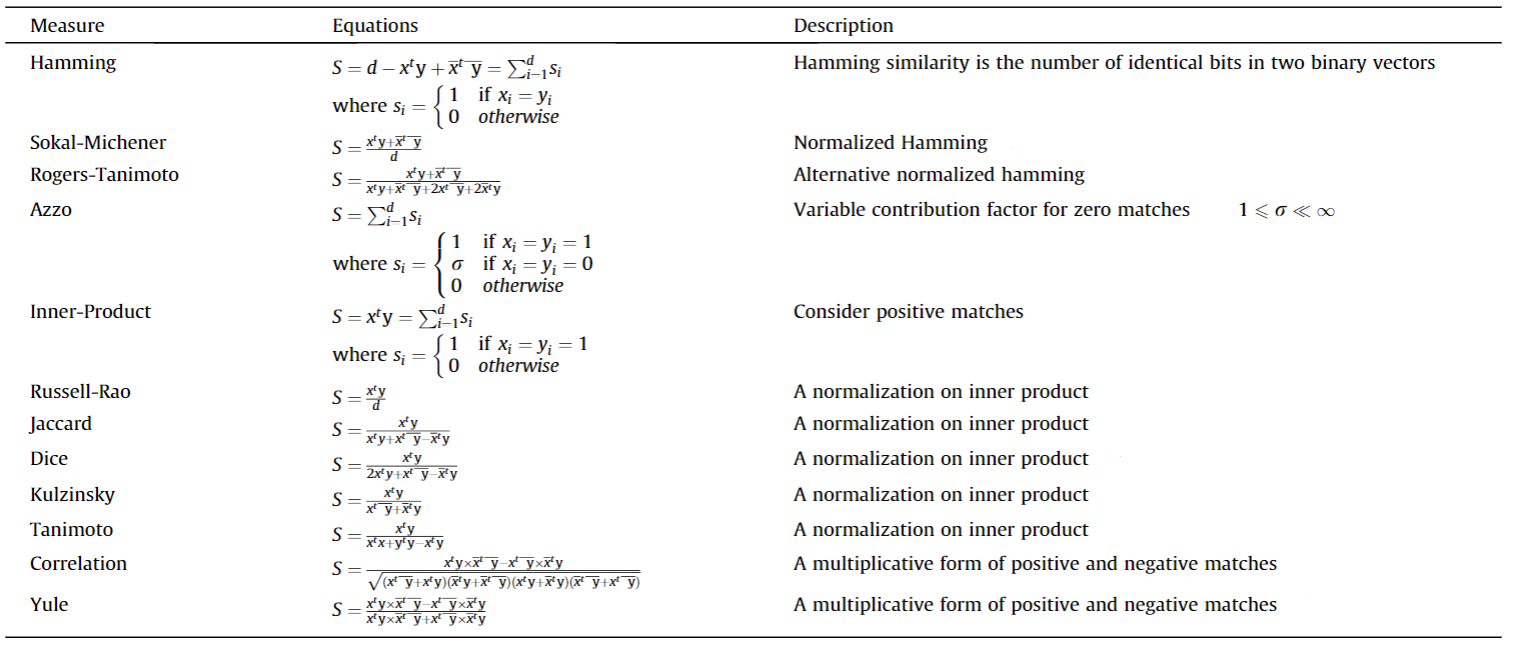
\includegraphics[scale=0.63]{section1/sims.png}
	\caption{انواع شباهت بین بردارهای دودویی}
	\label{fs7}
\end{figure}

\subsection{ترکیب شباهت‌های شبکه‌ای
\label{SNF}}

ترکیب شباهت‌های شبکه‌ای
\LTRfootnote{Similarity Network Fusion}\cite{Wang2014}\lr{(SNF)}
یک روش محاسباتی جدید برای ترکیب داده‌ها است. این روش انواع مختلفی از ویژگی‌ها (مانند ساختار شیمیایی، عوارض‌جانبی، آنزیم، منتقل‌کننده و غیره) را با مجموعه‌ی معینی از نمونه‌ها (به‌عنوان مثال داروها) ترکیب می‌کند. در این روش ابتدا برای هر یک از انواع داده‌ها یک شباهت نمونه ایجاد می‌شود و سپس با استفاده از یک روش جدید ترکیب شبکه،‌ شبکه‌ها یکپارچه می‌شوند. کار در فضای شبکه به
\lr{SNF}
اجازه می‌دهد تا از برخورد با مقیاس‌های مختلف، اریبی
\LTRfootnote{Bias}
 و نویز در انواع مختلف داده جلوگیری کند. روش ترکیب غیرخطی داده‌ها به
\lr{SNF} 
اجازه می‌دهد تا هم از اطلاعات رایج و هم از اطلاعات مکمل در انواع مختلف داده استفاده برد. شکل
\ref{fs8}
مثالی از مراحل
\lr{SNF} 
است.
 

\begin{figure}[!h]
	%\centering
	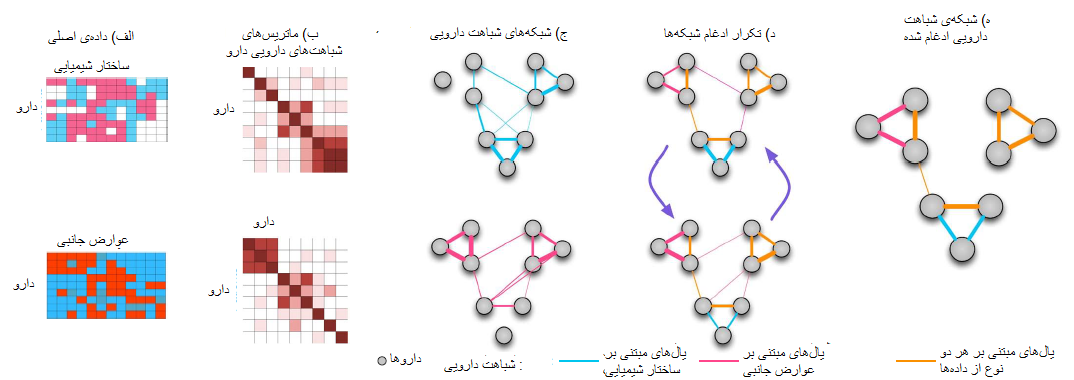
\includegraphics[scale=0.57]{section2/SNF.png}
	\caption{انواع شباهت بین بردارهای دودویی
    \cite{Wang2014}}
الف) نمایش نمونه‌ای از ویژگی ساختار شیمیای و ویژگی عوارض‌جانبی خارج از برچسب برای همان داروها. ب) ماتریس تشابه دارو-دارو برای هر نوع ویژگی. ج) شبکه‌های شباهت دارو-دارو، معادل داده‌های دارو-دارو.داروها توسط گره‌ها نمایان می‌شوند و شباهت‌های جفتی داروها توسط یال‌ها نشان داده ‌می‌شود. د) تلفیق شبکه توسط
\lr{SNF}
به‌طور مکرر، هر یک از شبکه‌ها را با اطلاعاتی از شبکه‌های دیگر به روز می‌کند و آن‌ها را در هر مرحله شبیه‌تر می‌کند. ه) ترکیب شبکه به‌صورت تکراری منجر به همگرایی می‌شود. رنگ یال نشان می‌دهد که کدام نوع داده به شباهت داده‌شده کمک کرده ‌است.
	\label{fs8}
\end{figure}

\section*{انتخاب مدل}

در این بخش توضیح مختصری از تاریخچه‌ی سامانه‌های توصیه‌گر و یادگیری عمیق داده می‌شود و سپس به بررسی تقسیم‌بندی آنها می‌پردازیم.

\section{سامانه‌های توصیه‌گر}

به کمک کامپیوتر‌ جوامع امروزی دستخوش تغییرات سریعی شده‌اند. بخش قابل توجهی از زندگی اجتماعی را کامپیوتر و اینترنت در برگرفته ‌است. یکی از موضوعات جدید مورد بحث حال حاضر دنیای کامپیوتر، سامانه‌های توصیه‌گر می‌باشد.

سامانه‌های توصیه‌گر
\LTRfootnote{Recommender Systems}
با اولین ظهورشان در زمینه فیلترینگ همکارانه
\LTRfootnote{Collaborative Filtering}،
حوزه تحقیقاتی مهمی را در اواسط دهه ۱۹۹۰ فراهم نمودند. دردهه‌های اخیر دو بخش صنعت و دانشگاه دستاوردهای جدیدی در زمینه سامانه‌های توصیه‌گر توسعه داده‌اند، با این ‌وجود علاقه‌مندی به این بخش هنوز در سطح بالایی است. تحقیقات این حوزه غنی بوده و نیاز مبرم به برنامه‌های کاربردی وجود دارد. این برنامه‌های کاربردی به‌منظور کمک به کاربران که با حجم زیادی از اطلاعات مواجه هستند و به‌منظور شخصی‌سازی اطلاعات توسعه داده شدند. به‌عنوان مثال از چنین برنامه‌هایی، می توان به سامانه‌های توصیه‌گر کتاب، سی‌دی و دیگر محصولات سایت آمازون
\LTRfootnote{Amazon}
و پیشنهاد فیلم توسط شرکت موی‌لنز
\LTRfootnote{MovieLens}
اشاره کرد.

تقریبا در اواسط دهه نود، مطالعه بر روی سامانه‌های توصیه‌گر به‌عنوان یک شاخه مستقل در تحقیقات مطرح شد. علت این توجه خاص، ابراز تمایل محققین، به‌استفاده از سامانه‌های توصیه‌گر برای حل مسئله جستجو در حجم فراوان اطلاعات بود. ظرفیت کامپیوترها در فراهم آوردن توصیه‌ها تقریبا از همان اوایل تاریخچه کامپیوتر‌ها شناخته شد. گراندی
\LTRfootnote{Grundy}،
کتابدار کامپیوتری گامی اولیه به سمت سامانه‌های توصیه‌گر خودکار برداشت. این کتابدار یک توصیه‌گر نسبتا ساده و اولیه بود که کاربران را به قالب‌هایی براساس مصاحبه کوتاه با استفاده از اطلاعات مستقیم‌کدشده
\LTRfootnote{Hard-coded}
درباره‌ی سلایق کتاب قالب‌های مختلف گروه‌بندی می‌کرد تا توصیه‌ها را تولید کنند. این کار ورود اولیه به فضای سامانه‌های توصیه‌گر قلمداد می‌شود.

در اوایل دهه نود میلادی، تکنیک پالایش مشارکتی
\LTRfootnote{Collaborative Refinement}
 به‌عنوان راه‌حلی برای مدیریت فضای اطلاعات بسیار زیاد آنلاین به‌وجود آمد. تپستری
\LTRfootnote{Tapestry}
یک سامانه پالایش مشارکتی دستی بود. این سامانه به کاربر اجازه انجام پرس‌وجو برای آیتم‌های موجود در حوزه اطلاعاتی مانند ایمیل بر اساس عقاید و اقدامات دیگر کاربران را می‌داد. این‌کار مستلزم تلاش از طرف کاربران بود و به آنها اجازه کنترل واکنش‌های خوانندگان قبلی در قسمتی از مکاتبات را می‌داد تا میزان ارتباط با آنها را تعیین کند. خیلی زود بعد از سامانه‌های خودکار پالایش مشارکتی، مکان‌یابی خودکار عقاید مرتبط و تجمع آنها برای دادن توصیه مطرح شد. گروپ لنز
\LTRfootnote{Group Lens}
از این تکنیک برای تعیین مقاله‌های یوزنت
\LTRfootnote{Usenet}
که احتمال دارد مورد علاقه کاربر خاصی باشد استفاده کرد. کاربران تنها به نمره‌دهی یا دیگر اقدامات قابل مشاهده می‌پرداختند. سامانه این فعالیت‌ها را با نمره‌ها یا اقدامات دیگر کاربران ترکیب می‌کرد تا نتایج شخصی‌شده تولید کند. با این سامانه‌ها، کابران برای دریافت پیشنهادات، قادرند بدون آنکه بدانند کاربران یا آیتم‌های دیگر سامانه چه‌چیزهایی هستند، اطلاعات مستقیمی از عقاید دیگر کاربران بدست آورند.

طی این دوره، سامانه‌های توصیه‌گر و پالایش مشارکتی تبدیل به موضوع مورد علاقه محققین حوزه‌های تعاملات انسان-رایانه، یادگیری ماشین و بازیابی اطلاعات شدند. این علاقه منجر به ایجاد سامانه توصیه‌گر در زمینه‌های مختلف شد. که از آن جمله می‌توان به
\lr{Ringo}
برای موسیقی، توصیه‌گر ویدیو 
\lr{BellCore}
برای فیلم‌ها و 
\lr{Jester}
برای لطیفه‌ها اشاره کرد. خارج از دنیای رایانه و درحوزه بازاریابی از توصیه‌گر‌ها، به‌دلیل توانایی آنها در افزایش فروش و بهبود تجربه مشتریان، استفاده کرده‌اند.

در اواخر دهه نود میلادی، پیاده‌سازی‌های تجاری فناوری توصیه‌گرها شروع به‌ظهور کردند. شاید معروف‌ترین کاربرد فناوری سامانه‌های توصیه‌گر وب‌سایت
\lr{Amazon.com}
باشد. براساس تاریخچه خرید، تاریخچه بازدید و موردی که کاربر درحال مشاهده است، وب‌سایت به کاربر مواردی را برای خرید توصیه می‌کند. از زمان به‌کارگیری فناوری توصیه‌گر توسط آمازون، در بسیاری از سیستم‌های تجارت الکترونیک و آنلاین، سامانه‌های توصیه‌گر (که اغلب بر اساس پالایش مشارکتی هستند)، ایجاد شده است. انگیزه مهم انجام این‌کار افزایش حجم فروش است زیرا ممکن است اگر کالا‌یی به مشتریان پیشنهاد شود آن را بخرند و درغیراینصورت ممکن است هرگز متوجه آن کالا نشده و آنرا نخرند. شرکت‌های بسیاری مانند 
\lr{NetPerceptions}
و 
\lr{Strands}
به‌دلیل فراهم‌کردن فناوری و خدمات توصیه به خرده‌فروشان آنلاین بوجود آمده‌اند.

زمانی‌که
\lr{Netflix}
جایزه 
\lr{Netflix Prize}
را در سال ۲۰۰۶ به منظور بهبود بخشیدن وضعیت توصیه‌های فیلمش برقرار کرد، تحقیق بر روی الگوریتم‌های سامانه‌های توصیه‌گر توجه بسیاری را به خودش جلب کرد. هدف این رقابت ساختن الگوریتم توصیه‌گری بود که بتواند الگوریتم
\lr{CineMatch}
که متعلق به خود
\lr{Netflix}
بود را با ۱۰٪ بهبود در آزمایشات آفلاین شکست دهد. این امر موجب ایجاد اقدامات گسترده‌ای در محیط دانشگاهی و سایر علاقمندان شد. جایزه یک میلیون دلاری ارزشی که فروشندگان برای دقت توصیه‌ها قائل هستند را نشان می‌دهد
\cite{HCI-009}.
به‌طور کلی دلیل استفاده از سامانه‌های توصیه‌گر و فیلترینگ اطلاعات، تبدیل اطلاعات موجود در مورد کاربران و اولویت‌های آن‌ها جهت پیش‌بینی علاقه آنها در آینده می‌باشد. در واقع در این سامانه از بین موارد مختلف بر اساس اینکه چه موردی برای کاربر جذاب است، مجموعه‌ی بزرگی از موارد مورد علاقه کاربران جمع‌آوری می‌شود. وب‌سایت‌های زیادی مانند
\lr{Amazon}، \lr{CDnow}، \lr{Ebay}
و غیره شروع به استفاده از سامانه‌های توصیه‌گر برای اهداف فروش الکترونیکی کردند. این وب‌سایت‌ها با توجه به اطلاعات و علایق مشتری به مشتری محصول مناسب سلیقه او را پیشنهاد می‌دهند که سبب افزایش رابطه میان وب‌سایت‌ها و مشتریان می‌شود. این باور وجود دارد که با ارائه توصیه‌های با کیفیت به مشتری و جلب رضایت او، وفاداری مشتری بهبود می‌یابد.

پیشرفت اینترنت باعث شده است اطلاعات آنلاین زیادی قابل دسترسی باشد. سامانه‌های توصیه‌گر می‌توانند مشکل انباشت اطلاعات را حل کنند. هدف این سامانه‌ها شناسایی سلیقه‌های کاربران و فیلترکردن داده‌های نامناسب از نظر آنهاست. نتیجه استفاده از سامانه‌های توصیه‌گر صرفه‌جویی زمانی جستجوهای کاربران است.
در شکل
\ref{recom1}
شمای کلی فرایند توصیه در سامانه‌های توصیه‌گر را مشاهده می‌کنید.


\begin{figure}
	\centering
	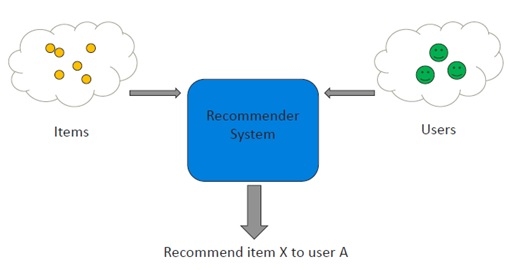
\includegraphics[scale=0.8]{section2/Recom1.jpg}
	\caption{شمای کلی فرایند توصیه در سامانه‌های توصیه‌گر}
	\label{recom1}
\end{figure}

\subsection*{تقسیم‌بندی سامانه‌های توصیه‌گر}

در کتاب‌های مختلف تقسیم بندی‌های مختلفی برای سامانه‌های توصیه‌گر وجود دارد. معمول‌ترین تقسیم‌بندی سامانه‌های توصیه‌گر را می‌توانید در شکل
\ref{Recom}
 مشاهده کنید.
 
\begin{figure}
\centering
\begin{tikzpicture}
        [edge from parent fork left, grow=left,
        every node/.style={fill=red!10,rounded corners},
        edge from parent/.style={gray,thick,draw}]
        \tikzstyle{block} = [ text width=4cm,text centered, minimum height=1em, fill=red!15]
        \tikzstyle{level 1}=[sibling distance=18mm,level distance=55mm] 
		\tikzstyle{level 2}=[sibling distance=15mm,level distance=55mm] 
        \node [block]{\lr{Recommendr Systems}}
	child{node[block] {\lr{Collabortive Filtrring}}
    	child{node[block]{\lr{User-Based}\rl{}}}
        child{node[block]{\lr{Item-Based}\rl{}}}
    	child{node[block]{\lr{Matrix Factorization}\rl{}}}
	}
	child{[sibling distance=5mm]node[block] {\lr{Content-Based }}
	}
	child{node[block] {\lr{Knowledge-Based}}
    	child{node[block]{\lr{Constrain-Based}\rl{}}}
    	child{node[block]{\lr{Case-Based}\rl{}}}
	}
	child{node[block] {\lr{Hybrid Approaches}}
	};

\end{tikzpicture}
	\caption{
تقسیم‌بندی سامانه‌های توصیه‌گر
\cite{HCI-009}
}
\label{Recom}
\end{figure}

\subsection{فیلترینگ همکارانه}
در روش فیلترینگ همکارانه
\LTRfootnote{Collabortive Filtrring}
پیشنهادات براساس شباهت‌های رفتاری و الگوهای عملکردی کاربرانی که شباهت‌های رفتاری و الگوهای مشابهی با کاربر فعلی در گذشته داشته‌اند، ارائه می‌شود. شاید تعریف آن کمی پیچیده باشد، به‌طور ساده روش فیلترینگ همکارانه بر این فرض استوار است که کاربرانی با نظرهای مشابه درباره یک مورد (منظور فیلم، عکس، موزیک یا هر چیز دیگری است که توصیه می‌شود) دارند، درباره موارد دیگر هم نظرات مشابه دارند. نمای کلی عمکرد این روش را در شکل
\ref{recom3}
مشاهده کنید. فیلترینگ همکارانه شامل سه بخش است که به بررسی آن‌ها می‌پردازیم:
\begin{figure}
	\centering
	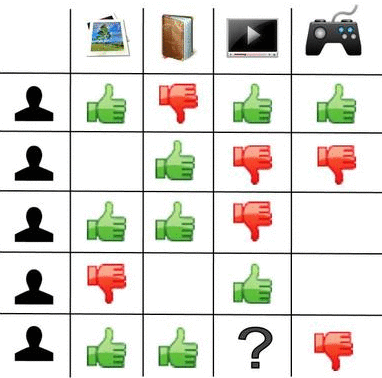
\includegraphics[scale=0.6]{section2/recom3.png}
	\caption{نمای کلی از روش‌های فیلترینگ همکارانه}
	\label{recom3}
\end{figure} 

\begin{itemize}
\item \textbf{مبتنی بر کاربر \LTRfootnote{User-Based}:}
در این روش افراد هم سلیقه با توجه به امتیازاتی که به موارد داده‌اند دسته‌بندی می‌شوند. از آنجا که کاربرانی با سلیقه شبیه به فرد مورد نظر بود و از  موارد یکسان خوششان آمده بود، پس آن مورد را به فرد مورد نظر نیز پیشنهاد می‌دهند.
\item \textbf{مبتنی بر آیتم \LTRfootnote{Item-Based}:}
در این روش وقتی یک کاربر یک مورد را می‌بیند، سامانه به‌صورت خودکار به دنبال آن می‌گردد که کاربرانی که قبلا این مورد را دیده‌اند بعد از آن چه موارد دیگری را دیده بودند. سپس سامانه آن موارد را به کاربر پیشنهاد می‌دهد. مثلا در سایت آمازون اگر یک گوشی بخرید بعد از آن، سامانه توصیه‌گر قاب گوشی و محافظ صفحه نمایشگر و چیزهایی مربوط به گوشی توصیه می‌کند.
\item \textbf{
تجزیه ماتریس
\LTRfootnote{Matrix Factorization}:\label{MatFactor}}
روش‌های مبتنی بر کاربر و مبتنی بر آیتم ساده هستند، اما معمولا روش‌های تجزیه ماتریس بیشتر تاثیرگذار هستند. زیرا این روش‌ها، ویژگی‌های پنهانی که در ارتباط میان کاربران و موارد وجود دارد را کشف می‌کنند. از این روش برای پیش‌بینی امتیازها در فیلترینگ همکارانه استفاده می‌کنند.
روش تجزیه ماتریس یک ماتریس ورودی را می‌گیرد و تلاش می‌کند دو ماتریس دیگر را به‌گونه‌ای بیابد که درصورت ضرب شدن در هم، ماتریس ورودی را تقریب بزنند. الگوریتم تجزیه ماتریس با مثال معروف توصیه‌ی کالاهای دیده نشده به کاربر معرفی می‌شود. در این حالت ماتریسی به‌نام
\lr{Y}
حاوی بازخوردهای کاربران برروی کالاها می‌باشد که شامل
\lr{m}
کاربر و
\lr{n}
کالا می‌باشد. مطابق شکل
\ref{Matrixfactorization}،
برای پیش‌بینی بازخورد کاربران روی کالاهای دیده ‌نشده ماتریس
$Y\epsilon R^{(m \times n)}$
به دو ماتریس
$A\epsilon R^{(m \times k)}$
و
$B\epsilon R^{(k \times n)}$
تقسیم می‌شود به‌طوری که
$ AB^T \approx Y$.
پارامتر قابل تنظیم
\lr{k}،
مربوط به تعداد ویژگی‌های نهفته
\lr{A} و \lr{B}
است كه
$k\ll m \times n$.

تجزیه ماتریس ویژگی‌های پنهان کاربران و کالاها را به شیوه‌ی بدون سرپرست مشخص می‌كند، كه برای فیلتركردن مشاركتی مفید است. به عنوان مثال، اگر بردارهای پنهان دو کاربر شبیه باشند، احتمال بالایی دارد که این کاربرها بازخوردهای یکسانی را به اشتراک بگذارند. به این ترتیب احتمال بازخورد مشابه روی کالاهای یکسان یا کالاهای مشابه بالاتر خواهد بود.

هدف يافتن بازخوردهای ناموجود در ماتریس
\lr{Y}
است كه تجزیه ماتریس می‌تواند به‌عنوان تکنیک تکمیل‌کننده‌ی ماتریسی مورد استفاده قرار گیرد. تصویری از تجزیه ماتریسی در شکل
\ref{Matrixfactorization}
نمایش داده شده‌است.

\begin{figure}[h!]
	\centering
	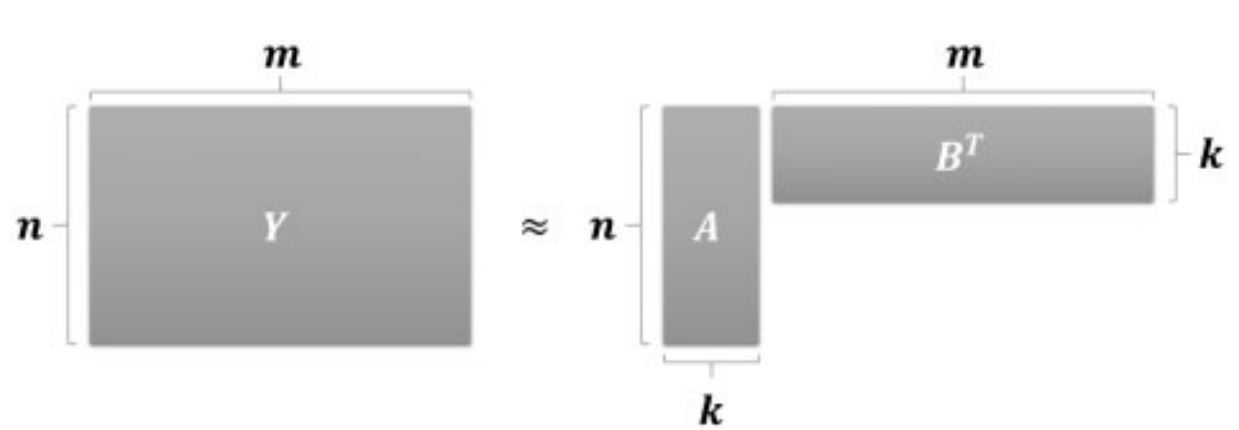
\includegraphics[scale=0.47]{section2/Matrixfactorization.jpg}
	\caption{
شرح مصور از تجزیه ماتریس}
\begin{flushright}
هدف این است که دو ماتریس ویژگی‌های پنهان
\lr{A} و \lr{B}
را به‌گونه‌ای بیابیم که ماتریس بازخورد
\lr{Y}
از ضرب این دو ماتریس بهتر بازسازی شود
\cite{Ezzat2018}.
\end{flushright}

	\label{Matrixfactorization}
\end{figure}


\end{itemize}
\par
\subsection{فیلترینگ مبتنی بر محتوا}

فیلترینگ مبتنی بر محتوا
\LTRfootnote{Content-Based}
از اطلاعات متنی و سابقه‌های کاربر برای تطابق موارد استفاده کرده و گزینه‌های مناسب را پیشنهاد می‌دهد. دانش اصلی‌ که در این تکنیک استفاده می‌شود شامل اطلاعات مواردی مثل ژانر، سال تولید و …  است که براساس این اطلاعات، مواردی که شبیه به هم هستند توصیه می‌شوند. در شکل 
\ref{recom4}
نحوه کلی عملکرد این روش را مشاهده می‌کنید. نمونه عمده این روش در وب‌سایت آمازون برای پیشنهاد کتاب‌ها بر اساس کلمات کلیدی کتاب‌های مشابه که سابقا توسط کاربر خریداری شده استفاده می‌شود.
\begin{figure}
	\centering
	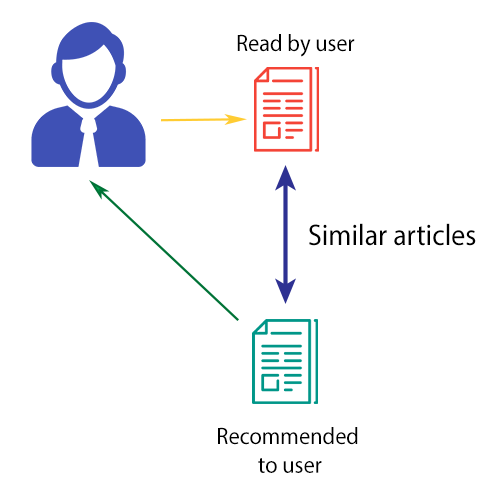
\includegraphics[scale=0.5]{section2/recom4.png}
	\caption{نمای کلی از روش‌های فیلترینگ مبتنی بر محتوا}
	\label{recom4}
\end{figure}
\par
\subsection{فیلترینگ مبتنی بر دانش}
دو روش توصیه‌گر قبلی محدودیت‌هایی دارند. محدودیت‌های استفاده از فیلترینگ همکارانه و فیلترینگ مبتنی بر محتوا را می‌توانید در قالب مثال بعدی ببینید. معمولا افراد به‌صورت مکرر ماشین، خانه و یا کامپیوتر نمی‌خرند. در این سناریوها یک سامانه فیلترینگ همکارانه خوب عمل نمی‌کند چون تعداد امتیازهای موجود بسیار کم است. علاوه‌بر‌این، محدوده زمانی نقش بسیار مهمی ایفا می‌کند. برای مثال، امتیازهایی که پنج سال قبل به یک کامپیوتر داده شده‌است به طور قطع برای توصیه مبتنی بر محتوا مناسب نیست.

روش فیلترینگ مبتنی بر دانش
\LTRfootnote{Knowledge-Based}
چالش‌های ذکرشده را حل می‌کند. سامانه‌های توصیه‌گر مبتنی بر دانش، نسل جدیدی از سامانه‌های توصیه‌گر هستند که مبتنی بر دانش موجود در رابطه با کاربران و موارد هستند. چنین سامانه‌هایی، پیشنهادات خود را بر پایه تفسیر و استنباط خود از سلایق و نیاز‌های کاربر ارائه می‌دهند و از دیدگاه تئوری نسبت به سایر روش‌های ذکر شده از دقت و کیفیت بیشتری برخوردار هستند. برای پیاده‌سازی چنین سامانه‌هایی نیاز به یک بستر و ساختار مبتنی بر دانش وجود دارد. در این گونه سامانه‌های توصیه‌گر موارد اولیه مورد استفاده برای تولید لیستی از پیشنهادها، دانش سامانه درمورد مشتری و کالا است. سامانه‌های مبتنی بر دانش از روش‌های مختلفی که برای تحلیل دانش قابل استفاده هستند بهره می‌برند. روش‌های رایج در الگوریتم‌های ژنتیک
\LTRfootnote{Genetic Algorithms}،
فازی
\LTRfootnote{Fuzzy}،
شبکه‌های عصبی
\LTRfootnote{Artificial Neural Networks} 
و … از جمله آنها است. همچنین، در این سامانه‌ها از درخت‌های تصمیم
\LTRfootnote{Design Tree}،
استدلال نمونه ‌محور
\LTRfootnote{Case-Based Reasonong}
و … نیز می‌توان استفاده کرد. روش مبتنی بر دانش خود به دو روش مبتنی بر محدودیت 
\LTRfootnote{Constrain-Based}
و مبتنی بر مورد 
\LTRfootnote{Case-Based}
تقسیم می‌شود. هر دو روش از لحاظ فرایند توصیه یکی هستند یعنی اول یک کاربر باید بطور دقیق درخواست خود را بگوید سپس سامانه تلاش ‌کند که یک راه‌حل تشخیص بدهد. سامانه حتی می‌تواند توضیح کوتاهی برای دلیل توصیه مورد بدهد. اما این دو روش از لحاظ تهیه دانش باهم تفاوت دارند. روش مبتنی بر مورد، آیتم‌های مشابه را با استفاده از میزان تشابه 
\LTRfootnote{Similarity Measure}
توصیه می‌کند اما روش مبتنی بر محدودیت، با توجه به قانون‌های توصیه‌ای که از قبل به طور صریح تعبیه شده فرایند توصیه را انجام می‌دهد.

\subsection{روش‌های ترکیبی}
روش‌های ترکیبی
\LTRfootnote{Hybrid Approaches}،
همانطور که اسم آنها پیداست ترکیبی از روش‌های قبلی است که سعی کرده با ترکیب روش‌ها از مزیت هریک از روش‌ها استفاده کند و محدودیت‌های آن‌ها را پوشش دهد.

\section{یادگیری عمیق}

الگوریتم‌های یادگیری عمیق
\LTRfootnote{Deep Learning}
زیرمجموعه‌ای از الگوریتم‌های یادگیری ماشین هستند که هدف آنها کشف چندین سطح از بازنمودهای توزیع‌شده
\LTRfootnote{Distributed Representation}
از داده ورودی است. اخیرا الگوریتم‌های یادگیری عمیق زیادی برای حل مسائل هوش مصنوعی سنتی ارائه شده‌اند. در این بخش مروری بر بعضی از الگوریتم‌های به‌روز این مبحث خواهیم داشت. درابتدا خلاصه‌ای از چندین روش یادگیری عمیق متفاوت و پیشرفت‌های اخیر آنها ارائه می‌شود و سپس به‌صورت خلاصه کاربردهای هر یک در زمینه‌های مختلف توضیح داده ‌می‌شود. در انتهای این بخش نیز گرایشات و مشکلات آینده در طراحی و آموزش شبکه‌های عصبی عمیق به‌صورت خلاصه ارائه می‌شود. طی سالهای اخیر, یادگیری عمیق به‌صورت گسترده مورد مطالعه قرار گرفته ‌است و به‌همین دلیل, تعداد زیادی از روش‌های مرتبط با آن به‌وجود آمده ‌است. به‌طورکلی, این روش‌ها بر اساس روش پایه‌ای که از آن مشتق شده‌اند به چهار دسته مختلف تقسیم می‌شوند
\cite{Guo Y2016}.

دسته‌بندی روش‌های یادگیری عمیق وکارهای انجام شده با هر یک از این روش‌ها در شکل 
\ref{dNN}
مشاهده می‌کنید.

%
\begin{figure}
\centering
\begin{tikzpicture}
        [ edge from parent fork left, grow=left,
        every node/.style={fill=red!10,rounded corners},
        edge from parent/.style={gray,thick,draw}]
        \tikzstyle{block} = [ text width=4cm,text centered, minimum height=1em, fill=red!15]
        \tikzstyle{level 1}=[sibling distance=58mm,level distance=55mm] 
		\tikzstyle{level 2}=[sibling distance=15mm,level distance=55mm] 
        \node [block]{\lr{Deep Learning Methods}}
	child{node[block] {\lr{RBM based Methodes}}
    	child{node[block]{\lr{Deep Belief Networks}\rl{\cite{G. Hinton2006}}}}
    	child{node [block]{\lr{Deep Boltzmann Machines}\rl{\cite{R.Salakhutdinov2009}}}}
    	child{node[block]{\lr{Deep Energy Models}\rl{\cite{J.Ngiam2011}}}}
	}
	child{[sibling distance=5mm]node[block] {\lr{CNN Based Methods }}
		child{node [block]{\lr{AlexNet}\rl{\cite{A.Krizhevsky2012}}}}
   		child{node[block] {\lr{Clarifai}\rl{\cite{M.D.Zeiler2014}}}}
   		child{node[block]{\lr{SPP}\rl{\cite{K.He2014}}}}
   		child{node[block]{\lr{VGG}\rl{\cite{K.Simonyan2015}}}}
    	child{node[block]{\lr{GoogLeNet}\rl{\cite{C.Szegedy2015}}}}
	}
	child{node[block] {\lr{Autoencoder Based Methodes}}
    	child{node[block]{\lr{Sparse Autoencoder}\rl{\cite{C.Poultney2006}}}}
    	child{node[block]{\lr{Denoising Autoencoder}\rl{\cite{P. Vincent2008}}}}
    	child{node[block]{\lr{Contractive Autoencoder}\rl{\cite{S. Rifai2011}}}}
	}
	child{node[block] {\lr{Sparse Codeing Based Methods}}
    	child{node[block]{\lr{Sparse Coding SPM}\rl{\cite{J. Yang2009}}}}
    	child{node[block]{\lr{Laplacian Sparse Coding}\rl{\cite{S. Gao2010}}}}	
    	child{node[block]{\lr{Local Coordinate Coding}\rl{\cite{K. Yu2009}}}}
    	child{node[block]{\lr{Super Vector Coding}\rl{\cite{X. Zhou2010}}}}
	};

\end{tikzpicture}
	\caption{دسته‌بندی روش‌های یادگیری عمیق و چند مثال از شبکه‌های هر دسته
\cite{Guo Y2016}
}
\label{dNN}
\end{figure}


\subsection{شبکه‌های عصبی کانولوشن}

شبکه‌های عصبی کانولوشن
\LTRfootnote{Convolutional Neural Networks(\lr{CNN})}
یکی از مهم‌ترین روش‌های یادگیری عمیق هستند که در آن‌ها چندین لایه با روشی قدرتمند آموزش می‌بینند. این روش بسیار کارآمد بوده و یکی از رایج‌ترین روش‌ها در کاربردهای مختلف است. تصویر کلی یک معماری شبکه عصبی کانولوشن در شکل
\ref{CNNarc} 
نمایش داده شده است. به‌طور کلی, شبکه
\lr{CNN}
از سه لایه اصلی تشکیل می‌شود که عبارتند از : لایه کانولوشن
\LTRfootnote{Convolution}،
لایه‌ی ادغام
\LTRfootnote{Pooling Layer}
و لایه‌ی تماما متصل
\LTRfootnote{Fully Connected}.
لایه‌های مختلف وظایف مختلفی را انجام می‌دهد. در شکل
\ref{CNNarc}
معماری کلی شبکه عصبی کانولوشن برای دسته‌بندی تصاویر به‌صورت لایه به لایه نمایش داده ‌شده ‌است
\cite{A. Krizhevsky2012}.
در هر شبکه عصبی کانولوشن دو مرحله برای آموزش وجود دارد. مرحله تغذیه رو به جلو
\LTRfootnote{Feed Forward}
و مرحله بازگشت به عقب
\LTRfootnote{Back Propagation}.
در مرحله اول تصویر ورودی به شبکه داده می‌شود و این عمل چیزی جز ضرب نقطه‌ای بین ورودی و پارامترهای هر نورون
\LTRfootnote{Neurons}
و نهایتا اعمال عملیات کانولوشن در هر لایه نیست، سپس خروجی شبکه محاسبه می‌شود. در اینجا به منظور تنظیم پارامترهای شبکه و یا به‌عبارت دیگر همان آموزش شبکه، از نتیجه خروجی جهت محاسبه میزان خطای شبکه استفاده می‌شود. برای اینکار خروجی شبکه را با استفاده از تابع خطا
\LTRfootnote{Loss Function}
با پاسخ صحیح مقایسه و میزان خطا محاسبه می‌شود. در مرحله بعدی براساس میزان خطای محاسبه شده، مرحله بازگشت به عقب آغاز می‌شود. در این مرحله گرادیان
\LTRfootnote{Gradient}
هر پارامتر با توجه به قائده زنجیره‌ای
\LTRfootnote{Chain Rule}
محاسبه می‌شود و تمامی پارامترها با توجه به تاثیری که بر خطای ایجاد شده در شبکه دارند تغییر پیدا می‌کنند. بعد از بروزرسانی شدن پارامترها مرحله بعدی تغذیه رو به جلو شروع می‌شود. بعد از تکرار تعداد مناسبی از این مراحل، آموزش شبکه پایان می‌یابد.
  
\begin{figure}[!h]
\centering
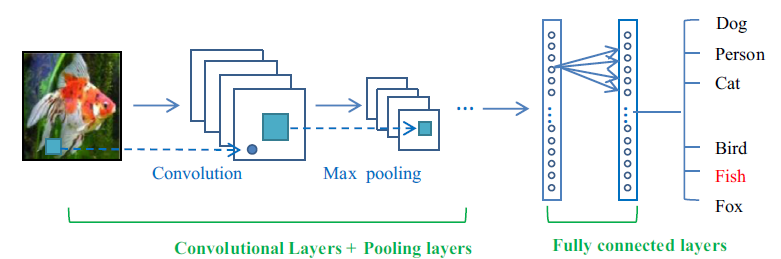
\includegraphics[scale=0.72]{section2/CNNarc.png}
	\caption{
طرح کلی از معماری یک شبکه عصبی کانولوشن
\cite{Guo Y2016}}
\label{CNNarc}
\end{figure}
\newpage
\subsection{ماشین بولتزمن محدود شده}
از لحاظ ساختاری، ماشین بولتزمن محدود شده
\LTRfootnote{Restricted Boltzmann Machines(\lr{RBM})}
یک شبکه عصبی مولد و تصادفی
\LTRfootnote{Generative Stochastic Neural Network}
همراه با محدودیت است. منظور از محدودیت آن است که واحدهای قابل مشاهده
\LTRfootnote{Visible Units}
و واحدهای پنهان
\LTRfootnote{Hidden Units}
یک گراف دو بخشی
\LTRfootnote{Bipartite Graph}،
تشکیل ‌دهند. واضح است که به لایه‌ی شامل واحدهای قابل مشاهده، لایه‌ی قابل مشاهده و به لایه‌ی شامل واحدهای پنهان، لایه پنهان می‌گویند و بر طبق محدویت 
\lr{RBM}
واحدهای یک لایه با هم هیچ‌گونه ارتباطی ندارند. این محدودیت باعث می‌شود الگوریتم‌های آموزش کارآمدتر باشند
\cite{Hinton GE1986}.

\begin{figure}[!h]
\centering
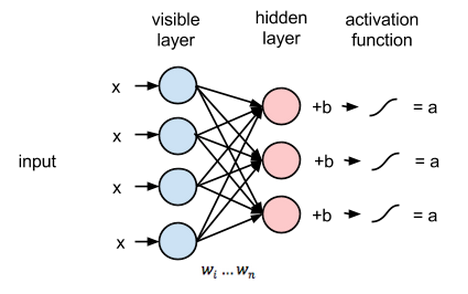
\includegraphics[scale=0.9]{section2/RBM.png}
	\caption{طرح کلی از معماری یک ماشین بولتزمن محدود شده}
\label{RBM}
\end{figure}

مطابق شکل
\ref{RBM}
هدف
\lr{RBM}
بازسازی تا حد امکان دقیق ورودی‌ها است. در مرحله‌ی تغذیه رو به جلو، ورودی‌ها توسط وزن‌ها و اریب‌ها اصلاح و برای فعال‌کردن لایه‌ی پنهان استفاده می‌شوند. از آنجایی که این مدل یک گراف دو بخشی است، واحدهای پنهان
\lr{H} 
و واحدهای قابل مشاهده
\lr{V} 
به‌صورت مشروط مستقل‌اند. بنابراین در معادله زیر:
\begin{equation}
P(HV_1) = P(H_1V_1)P(H_2V_2) ... P(H_nV_1)
\end{equation}
هم
$H$
و هم 
$V_1$
توزیع بولتزمن را برآورده می‌کنند. با ورودی
$V_1$
می‌توانیم
$H $
را از طریق 
$P(HV_1)$
به‌دست آوریم. به‌همین ترتیب می‌توانیم مقدار
$V_2$ 
را از طریق 
$P(HV_2)$
به‌دست آوریم. با تنظیم پارامترها، اختلاف بین
$V_1$
و
$V_2$
را به حداقل می‌رسانیم درنتیجه
$H$
حاصل، به‌عنوان ویژگی خوبی از
$V$
عمل می‌کند. در مقاله 
\cite{Hinton GE1986}
توضیح مبسوطی در این زمینه وجود دارد و راه عملی برای آموزش
\lr{RBM}
توضیح داده شده است.

\subsection{خودرمزنگار}
خودرمزنگار
\LTRfootnote{Autoencoder}
نوع خاصی از شبکه عصبی مصنوعی است که برای رمزگذاری کردن
\LTRfootnote{Encode} 
بهینه یادگیری مورد استفاده قرار می‌گیرد. در ساده‌ترین حالت شامل یک رمزگذار
\LTRfootnote{Encoder}
و یک رمزگشا
\LTRfootnote{Decoder}
به‌همراه فقط یک لایه پنهان می‌باشد. ورودی به رمزگذار داده شده و خروجی از رمزگشا استخراج می‌شود. به‌جای آموزش شبکه و پیش‌بینی مقدار هدف
\lr{Y}
به ازای ورودی
\lr{X}،
یک خودرمزنگار آموزش می‌بینید تا ورودی
\lr{X}
خود را بازسازی کند. بنابراین بردارهای خروجی همان ابعاد بردار ورودی را خواهند داشت.
\begin{figure}[!h]
\centering
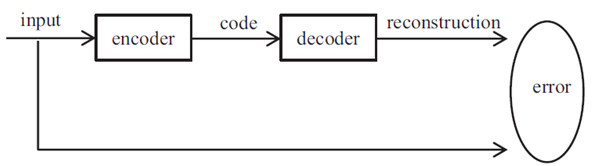
\includegraphics[scale=.8]{section2/autoC.png}
	\caption{فرآیند کلی یک خودرمزنگار\cite{Guo Y2016}}
\label{autoC}
\end{figure}
فرآیند کلی یک خودرمزنگار در شکل
\ref{autoC}
نشان داده شده است. در حین این فرآیند, خودرمزنگار با کمینه‌سازی خطای نوسازی
\LTRfootnote{Reconstruction Error}
بهینه می‌شود. کد متناظر همان ویژگی پیش‌بینی شده است. به‌طورکلی یک لایه‌ی تنها، قادر به دریافت ویژگی‌های متمایز از داده خام نیست. در حال حاضر محققان معمولا از خودرمزنگار عمیق استفاده می‌کنند که کد یادگرفته شده از خودرمزنگار قبلی را به خودرمزنگار بعدی جهت به انجام رساندن کار ارسال می‌کند.


\subsection{کدگذاری تنک}
کدگذاری تنک
\LTRfootnote{Sparse Coding}
نوعی روش بدون سرپرست است که به منظور یادگیری مجموعه خیلی کامل
\LTRfootnote{Over-Complete}
 از توابع پایه برای توصیف داده ورودی مورد استفاده قرار می‌گیرد
\cite{B.A. Olshausen۱997}.
این روش مزیت‌های متعددی دارد به‌عنوان مثال می‌توان به این موارد اشاره کرد :
 
۱) این روش قادر به بازسازی بهتر توصیه‌گر است زیرا از چندین پایه و ارتباط بین توصیه‌گرهای دارای پایه‌های مشترک‌ مشابه، استفاده می‌کند.
  
۲) پراکندگی این اجازه را می‌دهد که خصوصیت‌های برجسته داده ورودی دریافت شوند.

۳) از آنجا که این روش همسو با سیستم بینایی بیولوژیکی است، ویژگی‌های تنک ورودی‌ها نیز برای یادگیری مفید هستند.
   
۴) الگوها با ویژگی‌های تنک از لحاظ خطی بیشتر قابل جداسازی هستند.

برای مقایسه بین این چهار دسته از روش‌های یادگیری عمیق و بدست آوردن درک درستی از آنها، خلاصه‌ای از فواید و مشکلات هریک با توجه به خصوصیات متنوع آنها در جدول 
\ref{methodComp}
آمده است. در این جدول نه خصوصیت کلی وجود دارد. که در آن تعمیم‌پذیری 
\LTRfootnote{Generalization}
اشاره به موثر بودن روش مورد نظر برای سایر ورودی‌ها مانند تصویر, صدا و… و کاربردهای متنوع آنها مثل تشخیص صدا
\LTRfootnote{Speech Recognition}، 
تشخیص تصویر
\LTRfootnote{Visual Recognition} 
و …  دارد.  یادگیری بدون سرپرست 
\LTRfootnote{Unsupervised Learning}
اشاره به توانایی یادگیری خودکار مدل یادگیری عمیق با داده‌های ورودی بدون برچسب و بدون تفسیر نظارتی دارد.  یادگیری ویژگی 
\LTRfootnote{Feature Learning} 
مجموعه‌ای از روش‌هاست که به سیستم امکان اکتشاف خودکار ارائه‌های مورد نیاز برای تشخیص ویژگی یا دسته‌بندی بر اساس داده‌های خام را می‌دهد. زمان واقعی آموزش 
\LTRfootnote{Real-time Training} 
و زمان واقعی پیش‌بینی  
\LTRfootnote{Real-time Prediction}
به‌ترتیب به کارآیی فرآیندهای یادگیری و پیش‌بینی اشاره دارند. ادراک بیولوژیکی 
\LTRfootnote{Biological Understanding}
و توجیه نظری 
\LTRfootnote{Theoretical Justification} 
نشانگر، شالوده بیولوژیکی یا مبانی نظری روش مورد نظر است. تغییرناپذیری 
\LTRfootnote{Invariance}
اشاره به مقاومت روش مورد نظر در مقابل تبدیلاتی مانند دوران، تجانس  و تقارن دارد. مجموعه آموزشی کوچک 
\LTRfootnote{Small Training Set }
اشاره به توانایی یادگیری مدل عمیق با استفاده از تعداد کمی نمونه دارد. این نکته حائز اهمیت است که جدول 
\ref{methodComp} 
فقط یافته‌های کلی کنونی را نمایش می‌دهد و صبحتی از فرصت‌های آینده و یا نمونه‌های اختصاصی نمی‌کند. 


\begin{table}[h!]
\centering
\begin{tabular}{|c|c|c|c|c|}
\hline
خصوصیات       &
\lr{CNN} &  \lr{RBM}  &   \lr{AutoEncoder}  &   \lr{Sparse coding}
\\
\hline

تعمیم‌پذیری&بله & بله & بله & بله
\\
\hline

یادگیری بدون سرپرست&خیر & بله & بله & بله
\\
\hline

یادگیری ویژگی&بله & بله* & بله* & خیر
\\
\hline
 
زمان واقعی آموزش&خیر & خیر & بله & بله
\\
\hline

 زمان واقعی پیش‌بینی&بله & بله & بله & بله
\\
\hline

ادراک بیولوژیکی&خیر & خیر & خیر & بله
\\
\hline

توجیه نظری&بله* & بله & بله & بله
\\
\hline

تغییرناپذیری&بله* & خیر & خیر & بله
\\
\hline

مجموعه آموزشی کوچک&بله* & بله* & بله & بله
\\
\hline
\end{tabular}
	\caption{
مقایسه‌ی روش‌های مختلف شبکه‌های عصبی عمیق
\cite{Guo Y2016}
}
\begin{flushright}
توجه: «بله» اشاره به این دارد که دسته در این خصوصیت به‌خوبی عمل می‌کند. در غیراینصورت با «خیر» علامت‌گذاری می‌شود. «بله*» اشاره به توانایی ابتدایی و یا ضعیف دارد. 
\end{flushright}
	\label{methodComp}
\end{table}

\section{الگوریتم‌های پیشین در مسئله‌ی پیش‌بینی سه‌کلاسه برهم‌کنش دارو - دارو}

در این بخش الگوریتم‌های ارائه شده برای پیش‌بینی سه‌کلاسه برهم‌کنش دارو - دارو معرفی و نحوه‌ی عملکرد آنها به‌صورت مختصر شرح داده ‌می‌شود. هر سه الگوریتم معرفی‌شده، از روش‌های تجزیه ماتریس استفاده می‌کنند. روش تجزیه ماتریس یک مدل توصیه‌گر است که در بخش
\ref{MatFactor}
توضیح داده ‌شده ‌است. این روش با کمی تغییر یک راه‌حل مناسب برای مسئله‌ی پیش‌بینی برهم‌کنش دارو-دارو است که مثال‌هایی از آن در ادامه‌ی این بخش توضیح داده می‌شود.

 لازم به ذکر است که روش پیشنهادی این تحقیق، یک توصیه‌گر مبتنی بر شبکه عصبی عمیق است و از نظر ساختاری هیچ مشابهتی با روش‌های تجزیه ماتریس ندارد. تنها دلیل ذکر این روش‌ها محدود بودن مقالاتی است که در کار خود از داده‌های سه‌کلاسه  استفاده کرده‌اند (نگارنده تا زمان نگارش، این سه مقاله را یافته‌است). درفصل ۴ روند ارزیابی الگوریتم ارائه شده و نتیجه‌ی حاصل با نتایج این مقالات مقایسه می‌شود.


\subsection{چارچوب یکپارچه مبتنی بر تجزیه ماتریس سه‌کلاسه}

ایده اصلی مدل چارچوب یکپارچه مبتنی بر تجزیه ماتریس سه‌کلاسه
\LTRfootnote{Triple Matrix Factorization-Based Unified Framework(\lr{TMFUF})}،
ایجاد ارتباط بین ویژگی‌های داروهای شناخته شده با ساختار گراف برهم‌کنش‌های دارو – دارو است
\cite{Shi J-Y2018}.
چنین ارتباطی را به‌صورت رگرسیون کمترین مربعات جزئی
\LTRfootnote{Partial Least Square Regression}
مدل می‌کند که به‌عنوان یک مدل تجزیه ماتریس سه‌کلاسه
(\lr{TMF})
معرفی شده‌است. برای آموزش مدل رگرسیون از ویژگی عوارض جانبی خارج از برچسب داروها استفاده می‌شود. براساس ادعای نویسندگان این روش اولین روشی است که چارچوب یکپارچه
(\lr{UF})
ارائه می‌دهد. این چارچوب قادر به پیش‌بینی برهم‌کنش‌های دارویی برای هر دو مدل مسئله‌ی دوکلاسه و سه‌کلاسه است.

\begin{figure}[!h]
\centering
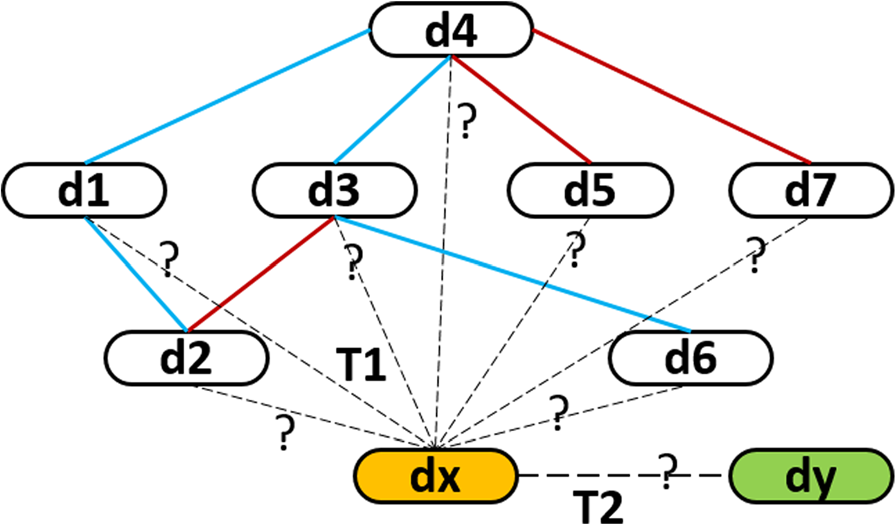
\includegraphics[scale=.5]{section2/TMFUFgraf.png}
	\caption{پیش‌بینی برهم‌کنش \lr{TMFUF}
\cite{Shi J-Y2018}}
\label{TMFUFgraf}
\end{figure}

با توجه به شکل
\ref{TMFUFgraf}
در گراف برهم‌کنش‌، داروها به‌عنوان گره‌ معرفی می‌شوند که داروهای شناخته شده از
$d1$
تا
$d7$
شماره‌گذاری شده‌اند. برهم‌کنش بین داروها با یال‌ها نشان داده می‌شوند و برهم‌کنش افزاینده و کاهنده به‌ترتیب توسط یال‌های قرمز و آبی مشخص شده‌اند. 
$d_x$
و
$d_y$
دو داروی جدید هستند که به‌صورت گره‌های مجزا و به‌ترتیب با برچسب‌های زرد و سبز مشخص می‌شوند. دو نوع پیش‌بینی، که با
$T1$
و
$T2$
برچسب گذاری شده‌اند، با خطوط نقطه‌چین نشان داده می‌شوند.
$T1$
احتمال برهم‌کنش داروی 
$d_x$
با داروهای شناخته‌شده را پیش‌بینی می‌کند، درحالی‌که
$T2$
احتمال برهم‌کنش داروی 
$d_x$
با داروهای جدید
$d_y$
را پیش‌بینی می‌کند. هر دو آنها پیش‌بینی می‌کنند که برهم‌کنش‌های بالقوه باعث افزایش یا کاهش رفتارهای دارویی می‌شوند.

\begin{figure}[!h]
\centering
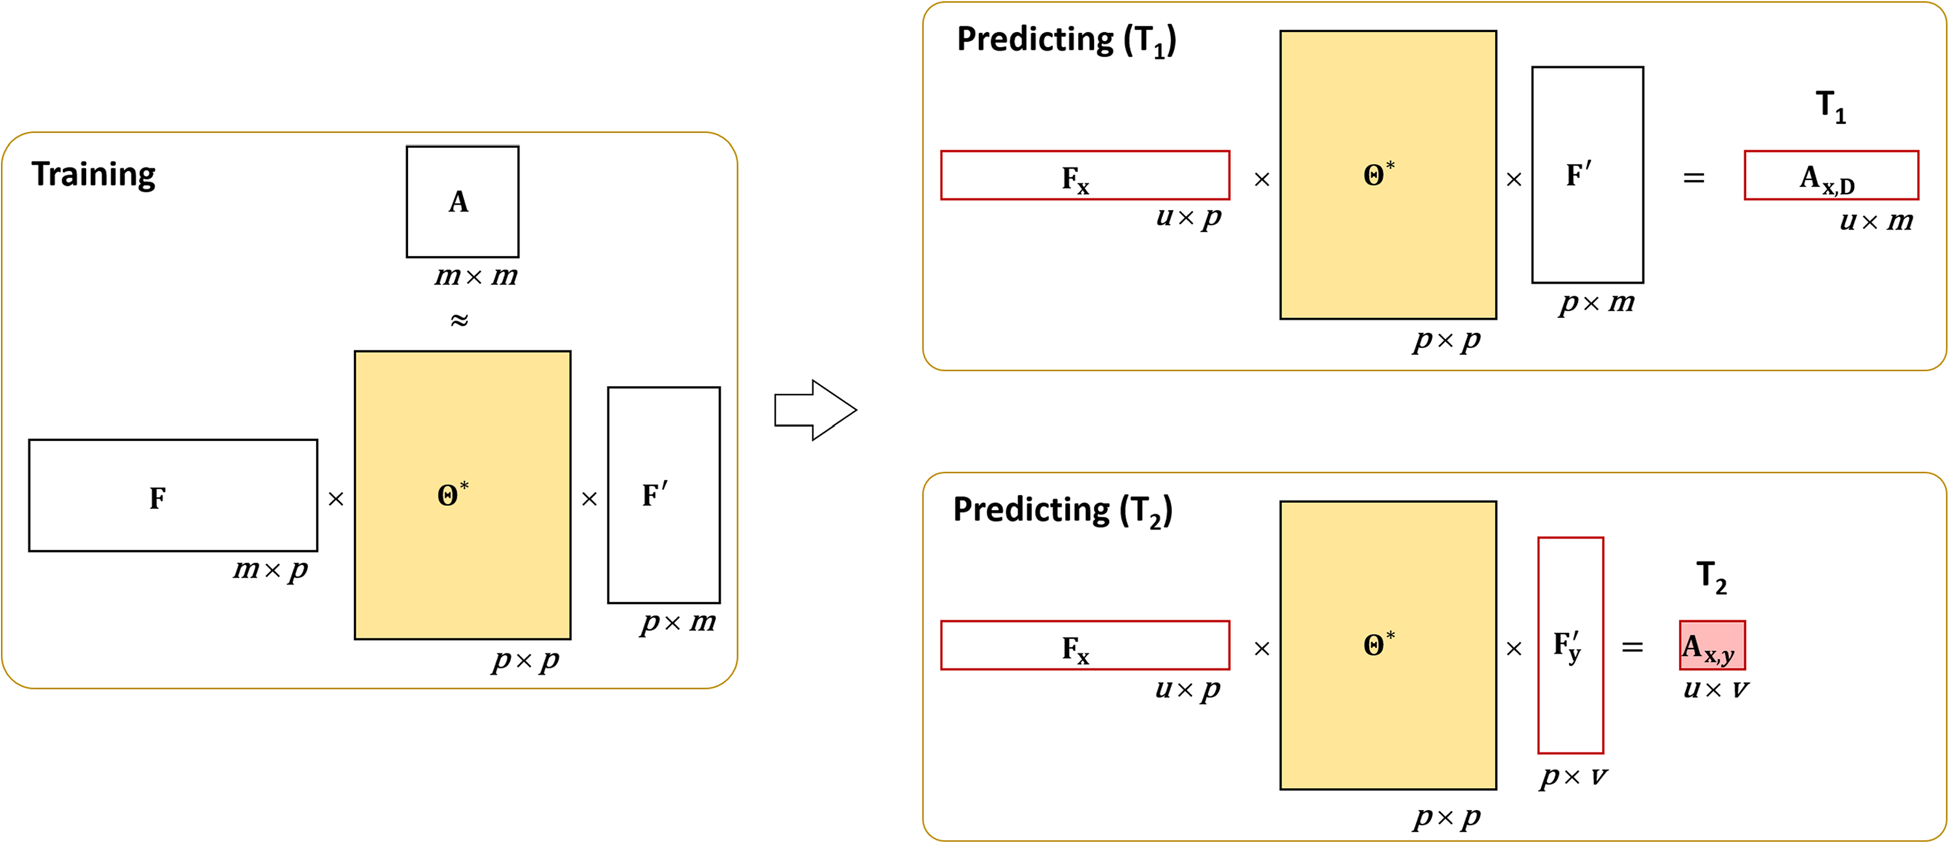
\includegraphics[scale=.3]{section2/TMFUFmodel.png}
	\caption{
ساختار مدل نظارت شده \lr{TMFUF}
\cite{Shi J-Y2018}}
\begin{flushright}
شکل سمت چپ روند آموزش و دو شکل سمت راست دو حالت پیش‌بینی را برای مدل
\lr{TMFUF}
نشان می‌دهند. این مدل برهم‌کنش‌های بین داروهای جدید و داروهای شناخته شده را پیش‌بینی می‌کند (بالا راست). همچنین برهم‌کنش‌های بین داروهای جدید با داروهای جدید را پیش‌بینی می‌کند (پایین راست).
\end{flushright}

\label{TMFUFmodel}
\end{figure}
با توجه به شکل 
\ref{TMFUFmodel}
در مرحله آموزش، ماتریس مجاورت برهم‌کنش‌ها
\lr{A}
و ماتریس ویژگی داروها
\lr{F}،
ماتریس تصویر متقارن
$\Theta$،
با استفاده از یک مدل رگرسیون 
\lr{Bi-Linear}\footnote{رگرسیون دو خطی شیب یک خط رگرسیون برای Y نسبت به X است که به عنوان یک تابع خطی از متغیر سوم Z تغییر می‌کند.}،
به‌صورت زیر ساخته می‌شود.
\begin{equation}
\begin{aligned}
A = F\cdot\Theta\cdot{F^\prime}
\label{TMFUF1}
\end{aligned}
\end{equation}
از آنجا که مقدار 
$\Theta$
را نمی‌توان مستقیما با معکوس‌گیری معادله
\ref{TMFUF1}
به‌دست آورد، بنابراین روش جدیدی برای حل آن پیشنهاد شد. در روش پیشنهادی فرض می‌شود فضای ویژگی نهان کم بعدی وجود دارد که در آن هر دارو توسط یک بردار نهان نشان داده می‌شود و ماتریس حاصل ضرب داخلی بین داروها با ماتریس برهم‌کنش داروها ارتباط مستقیم دارد. به‌علاوه فرض می‌شود ویژگی‌های نهفته داروها با ویژگی مشاهده شده آنها مرتبط است. حل
$\Theta$
به شرح زیر است.
\begin{equation}
\begin{aligned}
\begin{split}
A^*_d= arg min{\parallel{A-{A_d\cdot{A^\prime}_d}\parallel}^2}, 
\\
B^* = arg min{\parallel{{A^*_d} - {F \cdot B}\parallel}^2}
\\
\Theta ^* = B^*\cdot ( B^*) ^ \prime
\end{split}
\end{aligned}
\end{equation}
$A_d$
ماتریس برهم‌کنش پنهان است که هر سطر آن نشان‌دهنده‌ی بردار ویژگی یک دارو در فضای نهفته‌است و باتوجه به متقارن بودن 
\lr{A}، $A_d$
را با الگوریتم تجزیه به مقدار ویژه به‌دست می‌آوریم. 
$A^*_d$
فضای پنهان را با تجزیه ماتریس بازتاب می‌دهد. 
\lr{B}
ماتریس ضرایب رگرسیون است که رابطه‌ای بین فضای ویژگی‌های مشاهده شده و فضای ویژگی پنهان داروها ایجاد می‌کند. برای به‌دست آوردن آن از رگرسیون کم‌ترین مربعات جزئی استفاده می‌شود. 

بعد از
$\Theta^*$،
مدل پیش‌بینی
$T1$
و
$T2$
به شرح زیر استخراج می‌شود.
\begin{equation}
\begin{aligned}
\begin{split}
A_{x,D}={F_x \cdot {\Theta^*}\cdot{F^\prime}},
\\
A_{x,y}={F_x \cdot {\Theta^*}\cdot{F^\prime}_y}
\end{split}
\end{aligned}
\end{equation}

در مدل کردن سه‌کلاسه، تغییرات داروشناسی ناشی از برهم‌کنش‌ها ثبت می‌شود که پیش‌بینی این مدل با ارزش‌تر و از نظر داروشناسی معتبرتر است. علاوه‌براین، راه حلی یکپارچه برای پیش‌بینی برهم‌کنش دارویی در دو سناریو ارائه می‌دهد. در سناریوی اول توانایی مدل برای بازگردانی برهم‌کنش بین داروهای شناخته‌شده سنجیده می‌شود. در سناریوی دوم توانایی مدل برای بازگردانی برهم‌کنش بین داروهای شناخته‌شده و داروی جدید محک می‌خورد. بدیهی است که داروهای جدید با داروهای قبلی هیچ برهم‌کنشی ندارند و اصطلاحا اطلاعات کمتری از آن‌ها وجود دارد. این مدل در هر دو سناریوی مسئله‌ی سه‌کلاسه موظف است نوع برهم‌کنش را پیش‌بینی کند. برهم‌کنش‌های احتمالی جفت داروها افزاینده یا کاهنده هستند. مزیت دیگر روش 
\lr{TMFUF}
در توانایی نشان‌دادن وجود تاثیر معنادار جفت ویژگی‌های دارویی (عوارض جانبی خارج از برچسب هر دو دارو) در پیش‌بینی برهم‌کنش دارویی است.

\subsection{
پیش بینی برهم‌کنش دارو-دارو بر اساس تجزیه ماتریس غیرمنفی}

در روش پیش بینی برهم‌کنش دارو-دارو بر اساس تجزیه ماتریس غیرمنفی
\LTRfootnote{Drug-Drug Interactions Via Semi- None Negative Matrix Factorization} (\lr{DDINMF})
یک مدل نظارت شده برای انجام پیش‌بینی برهم‌کنش دارو-دارو ایجاد می‌شود.
\cite{Yu H2018}

\begin{figure}[!h]
\centering
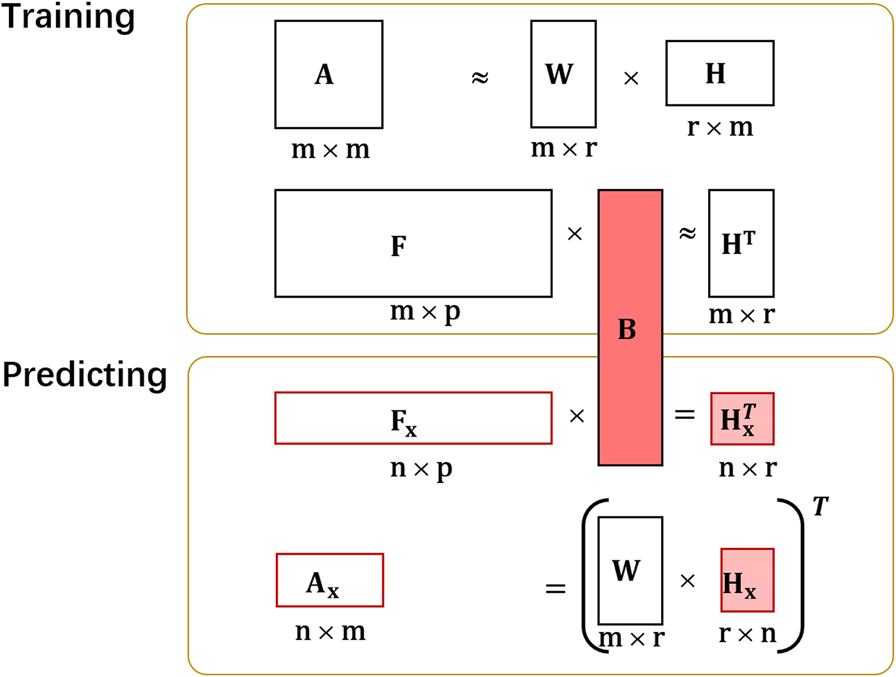
\includegraphics[scale=.4]{section2/DDINMF.png}
	\caption{بررسی اجمالی \lr{DDINMF}
\cite{Yu H2018}}
\label{DDINMF}
\end{figure}
در این روش برهم‌کنش‌ها براساس خواص ساختار شبکه‌ی دارویی  و در روند تجزیه ماتریس آموزش داده می‌شوند. سپس برای ایجاد رابطه بین ویژگی‌های دارویی ( ساختار شیمیایی و عوارض جانبی ) و گراف برهم‌کنش داروها از رگرسیون کم‌ترین مربعات جزئی استفاده می‌شود. این ارتباط در فرآیند پیش‌بینی برهم‌کنش بین داروی جدید و داروهای موجود به‌کار می‌رود. با توجه به شکل
\ref{DDINMF}
مدل 
\lr{DDINMF}
شامل دو مرحله است.

۱) مرحله‌ی آموزش: در این مرحله ماتریس مجاورت ساخته ‌شده بین داروهای شناخته شده به دو ماتریس پایه
\lr{W}
و ماتریس ویژگی پنهان
\lr{H}
توسط 
$A_{m\times m}\approx{W_{m\times r}\times{H_{r\times m}}}$
تجزیه می‌شود. در اینجا 
\lr{r}
اندازه‌ی بعد فضای پنهان است. سپس رابطه‌ای بین ماتریس ویژگی‌ ورودی
\lr{F}
و ماتریس ویژگی پنهان
\lr{H}
توسط رگرسیون به‌صورت 
$(H^T)_{m\times r}={F_{m\times P}\times{B_{p\times r}}}$
مدل می‌شود که 
\lr{B}
ماتریس ضرایب رگرسیون است.

۲) مرحله‌ی پیش‌بینی: در این مرحله، ماتریس ضرایب
\lr{B}
ماتریس ویژگی ورودی داروهای جدید
$F_x$ 
را به ماتریس ویژگی پنهان جدید به‌صورت
${H^T_x}={F_x\times B}$
می‌نگارد
\LTRfootnote{Map}.
سپس با استفاده از ماتریس ویژگی پنهان جدید، پیش‌بینی بین داروهای جدید و داروهای شناخته شده توسط
${A_x}={(W\times{H_x})}^T$
ایجاد می‌شود.

 رویکرد ارائه ‌شده شامل دو روش تجزیه ماتریس غیر منفی
\LTRfootnote{None Negative Matrix Factorization}(\lr{NMF})
 و تجزیه ماتریس نیمه-غیر منفی
\LTRfootnote{Semi- None Negative Matrix Factorization}(\lr{Semi-NMF})
 است. 
 
مدل 
\lr{NMF}
از قید غیرمنفی بودن هر دو ماتریس حاصل از تجزیه استفاده می‌کند تا ماتریس اصلی را تقریب بزند. تابع هدف و تابع‌ بروز‌رسانی
\lr{H} و \lr{W}
به شرح زیر است.
\begin{equation}
\begin{aligned}
min||X-WH||_F^2 =\sum_{i,j}{( x_{ij} -\sum_{k=1}^r w_{ik} h_{ki}})^2, 
W,H\geq0
\end{aligned}
\end{equation}

\begin{equation}
\begin{aligned}
\begin{split}
{w_{ik}}\longleftarrow{w_{ik}\dfrac{(XH^T)_{ik}}{(WHH^T)_{ik}}} 
\\
{h_{ik}}\longleftarrow{h_{ik}\dfrac{(X^TW)_{kj}}{(H^TW^TW)_{kj}}}
\end{split}
\end{aligned}
\end{equation}
که در آن
$w_{ik}$
مراکز خوشه در شبکه‌ی دارویی و
$h_{ik}$
شاخص
\LTRfootnote{Indicator}
خوشه یا عضویت نمونه‌ها در شبکه را مشخص می‌کند.
 
مدل 
\lr{NMF}
محدویت قوی نامنفی بودن را دارد، لذا نمی‌تواند برای حل مسئله‌ی سه‌کلاسه به‌صورت مستقیم استفاده شود. پس لازم است هربار جداگانه روی پیش‌بینی برهم‌کنش‌های افزاینده و کاهنده کار کند. اما مدل
\lr{Semi-NMF}
با استفاده از قید غیرمنفی بودن تنها یکی از ماتریس‌های فضای نهان این امکان را دارد که برای آموزش و پیش‌بینی مسئله‌ی سه‌کلاسه به‌کار رود. روش 
\lr{Semi-NMF}
داروها را خوشه‌بندی کرده و اطلاعات و ویژگی‌های بیشتری از داروها را، درکنار پیش‌بینی برهم‌کنش دارویی، ارائه می‌دهد. در این روش نویسندگان برای پیش‌بینی برهم‌کنش داروهای جدید، از الگوریتم متفاوتی برای به حداقل رساندن تابع هدف استفاده می‌کنند.
\begin{equation}
\begin{aligned}
\begin{split}
{W}\longleftarrow{XH^\dagger}
\\
{H}\longleftarrow{H\odot{\sqrt{\dfrac{(W^TX)^{pos}+[(W^TW)^{neg}H]_{ik}}{(W^TX)^{neg}+[(W^TW)^{pos}H]_{ik}}}}}
\end{split}
\end{aligned}
\end{equation}
که در آن
$H^\dagger$
ماتریس شبه وارون
\lr{H}
است.
$A^{pos}$
و
$A^{neg}$
به ترتیب ماتریس‌هایی هستند که مولفه‌های منفی و مثبت ماتریس 
\lr{A}
را با صفر جایگزین کرده اند:
\begin{equation}
\begin{aligned}
\forall i,j
A_{ij}^{pos}=\dfrac{|A_{ij}|+A_{ij}}{2}  ,   
A_{ij}^{neg}=\dfrac{|A_{ij}|-A_{ij}}{2} 
\end{aligned}
\end{equation}
این رویکرد قادر به پیش‌بینی برهم‌کنش‌های دوکلاسه معمولی و برهم‌کنش‌های جامع سه‌کلاسه است.

از همه مهم‌تر، باید این نکته‌ی کلیدی را درنظر داشته باشیم که شبکه‌ی دوکلاسه برهم‌کنش‌های دارو-دارو به هیچ‌وجه حاوی اطلاعاتی در مورد برهم‌کنش‌های افزاینده و کاهنده نیست، اما بررسی درجه‌ی رئوس در شبکه‌ی سه‌کلاسه جامع اطلاعات مفیدی از انواع برهم‌کنش‌ها ارائه می‌دهد که می‌تواند به درک بهتر برهم‌کنش‌های دارویی بیانجامد. نحوه‌ی چینش برهم‌کنش‌ها در شبکه سه‌کلاسه جامع نشان می‌دهد بروز علائم ناشی از برهم‌کنش‌های افزاینده و کاهنده تصادفی نیست و از قواعد و قوانین خاصی پیروی می‌کند.


گراف سه‌کلاسه‌ی جامع برهم‌کنش یک شبکه با ساختاری متعادل
\LTRfootnote{Structural Balance}
است. نظریه‌ی تعادل ضعیف
\LTRfootnote{Weakly Balance Theorem}
بیان می‌کند که گره‌های شبکه‌ را می‌توان در
\lr{k}
خوشه قرار داد، به‌طوری که اکثر یال‌های درون هر خوشه افزاینده و اکثر یال‌های بین خوشه‌ها کاهنده باشند
\cite{Davis1967}.


\subsection{تنظیم متعادل تجزیه ماتریس نیمه غیر منفی}

روش موسوم به تنظیم متعادل تجزیه ماتریس نیمه غیر منفی
\cite{Shi J2019} 
\LTRfootnote{Balance Regularized Semi-Nonnegative Matrix Factorization} (\lr{BRSNMF})
تلاشی برای تقویت روش
\lr{Semi-NMF}
پیشین است و علاوه بر آن ساختار اساسی تعادل ضعیف شبکه جامع سه‌کلاسه را نشان می‌دهد. این مدل از روابط ساختاری برای حل دو مسئله استفاده می‌کند: 
 
۱) کشف انجمن\LTRfootnote{Community}‌های دارویی و تقویت توان انجمن‌یابی
\LTRfootnote{Community Detection}

۲) پیش‌بینی جامع برهم‌کنش‌ها. 

طبق پیش‌بینی نویسندگان مقاله، شبکه‌ی برهم‌کنش دارویی را می‌توان به انجمن‌ها و گروه‌هایی تقسیم‌بندی کرد. به‌شکلی بیشتر یال (برهم‌کنش) های درون انجمن دارویی افزاینده و بیشتر یال‌های بین انجمنی کاهنده باشند. در این راستا دو معیار تنظیم گراف،
$Gr_1$
برای درون انجمن‌ها و
$Gr_2$
برای بین انجمن‌ها به‌صورت زیر معرفی شدند . همچنین، این دو معیار تنظیم از به وجود آمدن خوشه‌هایی با گره‌های کم جلوگیری می‌کنند.
\begin{equation}
\begin{aligned}
\begin{split}
Gr_1 = min \sum^k_{c=1}\dfrac{{h^T_c}{A^-}{h_c}}{{h^T_c}{h_c}},
\\
Gr_2 = min \sum^k_{c=1}\dfrac{{h^T_c}{L^+}{h_c}}{{h^T_c}{h_c}}
\end{split}
\end{aligned}
\end{equation}
که درآن
$h_c$,\lr{c}امین
ستون برداری در 
\lr{H}
است و 
$L^+=D^+-A^+$
است که در آن
$D^+$
ماتریس قطری
$A^+$
است و داریم
$\forall i,j a^+_{ij}=\dfrac{|a_{ij}|+a_{ij}}{2} , a^-_{ij}=\dfrac{|a_{ij}|-a_{ij}}{2}$.

با ترکیب 
$Gr_1$
و
$Gr_2$
و پس از ساده‌سازی داریم:
\begin{equation}
\begin{aligned}
Gr \equiv max { tr(H^T(\sigma I-\eta (A^-+L^+))H)}=max{ tr(G)}
\end{aligned}
\end{equation}
که در آن
$\sigma,\eta>0$
اندازه خوشه‌ها را کنترل می‌کند.

همچنین، معیار تنظیم 
\lr{Sr}
برای کنترل پراکندگی
\lr{H}
به‌صورت زیر طوری تعریف می‌شود که گره‌های دارو در شبکه برهم‌کنش به کمترین انجمن‌های ممکن تعلق داشته باشند:
\begin{equation}
\begin{aligned}
Sr= \sum^m_j||h_j||_1^2 =tr(HlH^T)=tr(s)
\end{aligned}
\end{equation}
که در آن
\lr{l}
ماتریس
$k \times k$
یی است که تمام درآیه‌های آن یک است.

پس از یکپارچه‌سازی معیارهای تنظیم به ماتریس درجه پایین، تابع هدف 
\lr{BRSNMF}
به شرح زیر است.
\begin{equation}
\begin{aligned}
min||A-WH^T||_F^2 +\alpha \cdot tr(S) - \beta \cdot tr(G), 
h_{ij}\geq0 , \forall i,j \in [1,...,m]
\end{aligned}
\end{equation}
برای حل و بروز‌رسانی از قوانین زیر استفاده می‌شود.
\begin{equation}
\begin{aligned}
\begin{split}
{W}\longleftarrow{AH(H^TH)^{-1}}
\\
{H}\longleftarrow{H\odot(N\div D)^{\dfrac{1}{2}}}
\\
N=(A^TW)_++(HW^TW)_-+\beta \eta(L^+H)_-+\beta \sigma H
\\
D=(A^TW)_-+(HW^TW)_+\alpha Hl+\beta \eta A^-H+\beta\eta(L^+H)_+
\end{split}
\end{aligned}
\end{equation}
که عملگرهای
$X_+$
و
$X_-$
بصورت
$X_+=\dfrac{|A|+A}{2}$
و
$X_-=\dfrac{|A|-A}{2}$
تعریف می‌شوند.


این تغییرات دو خصوصیت زیر را به نتایج حاصل از اجرای روش تحمیل کرد. 
 
۱) ارتباطات بین انجمنی بیشتر از نوع کاهنده باشد که کمک کند دورهای متعادل در درون انجمن‌ها تشکیل شده و دورهای نامتعادل در بین انجمن‌ها باشد. 

۲) از ایجاد خوشه‌هایی با تعداد گره‌های کم جلوگیری شود که باعث شد نسبت به
\lr{Semi-NMF}
انجمن‌های خیلی چاق یا خیلی لاغر تشکیل نشود. 

\begin{figure}[!h]
\centering
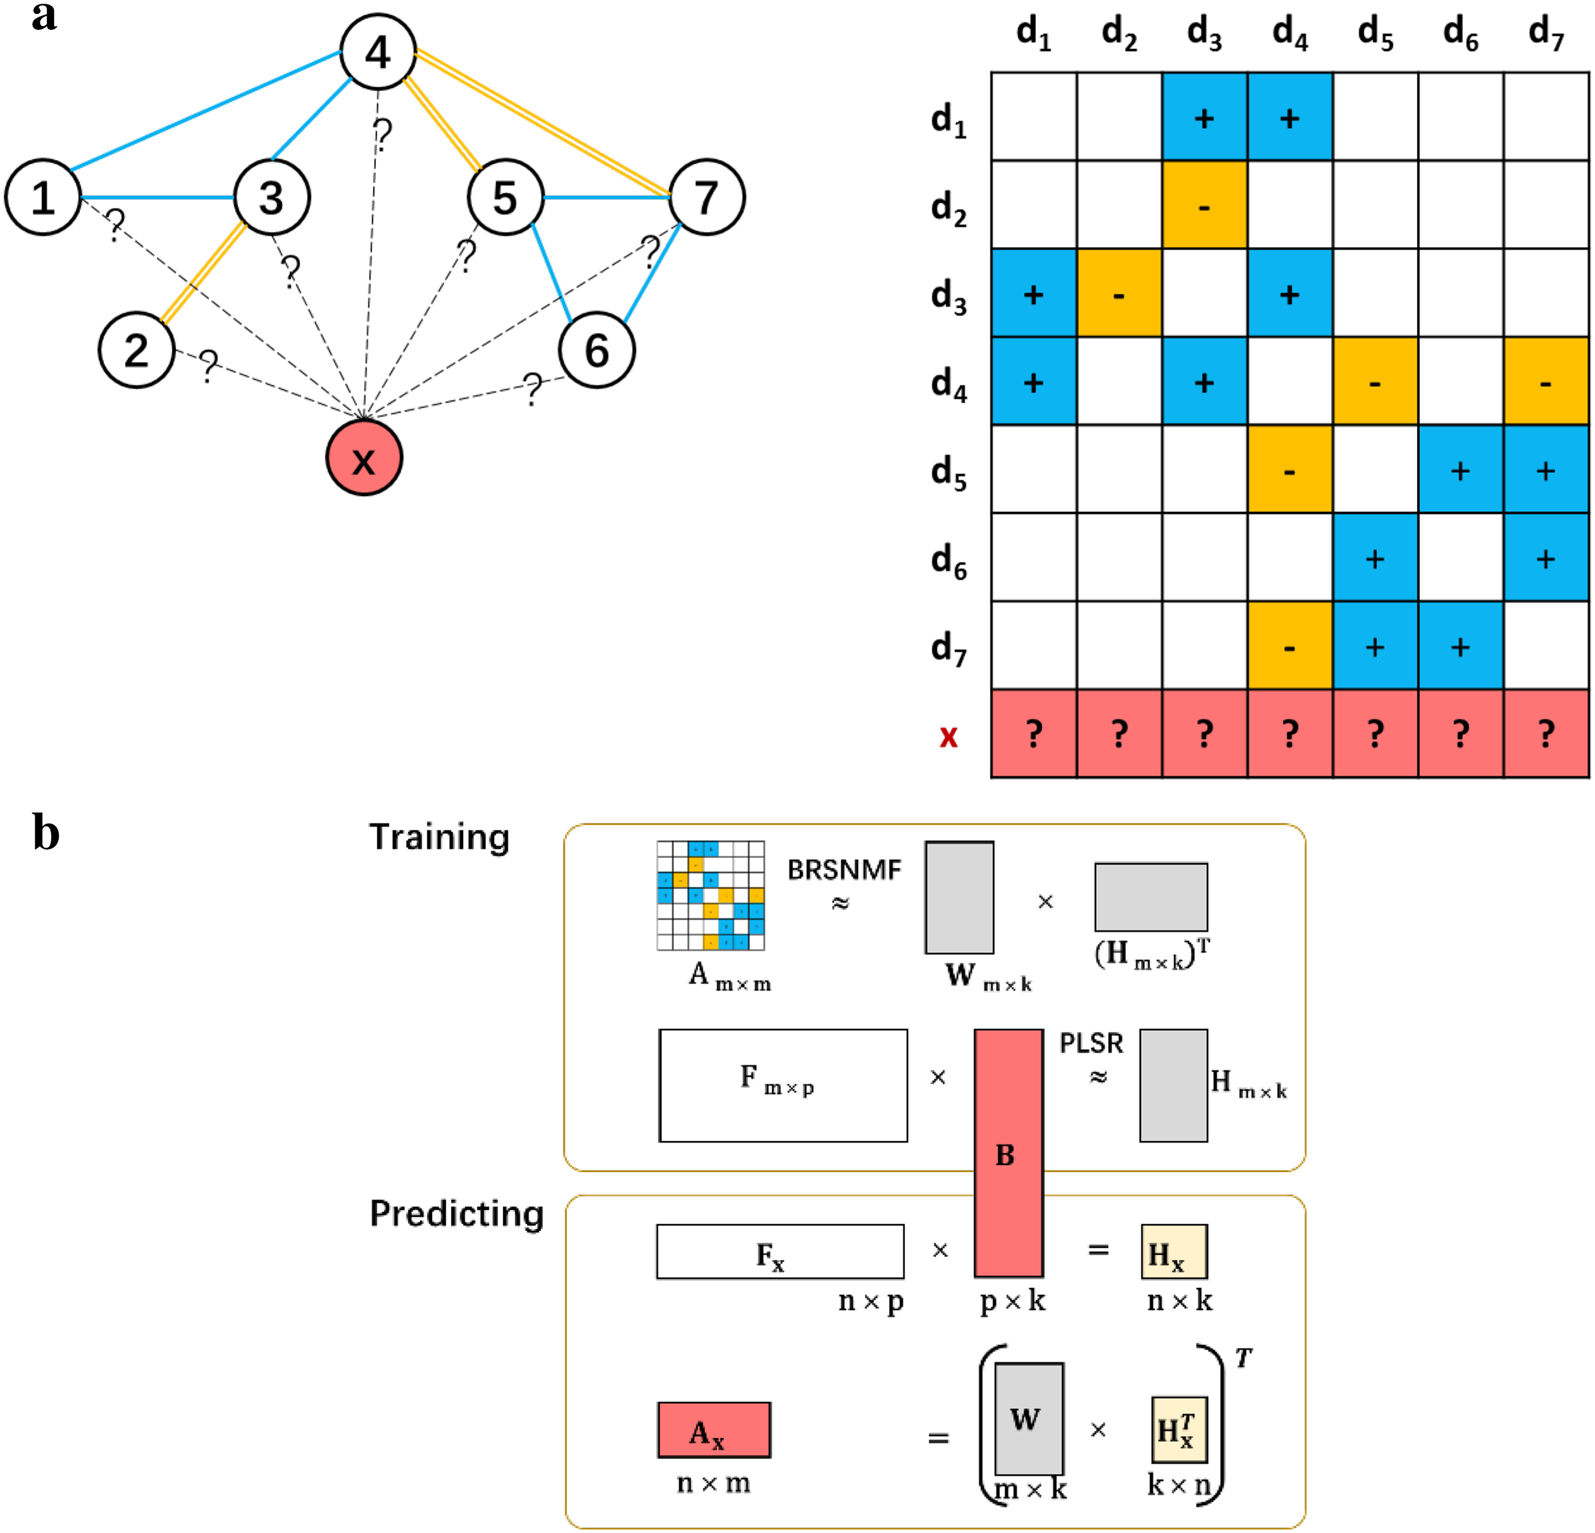
\includegraphics[scale=.3]{section2/BRSNMF.png}
	\caption{پیش‌بینی برهم‌کنش جامع در سناریو شروع سرد \lr{BRSNMF}
\cite{Shi J2019}}
\label{BRSNMF}
\end{figure}

اتخاذ چارچوب مسئله شروع سرد
\LTRfootnote{Cold Start}\cite{Yu H2018}
در رویکرد مبتنی بر
\lr{BRSNMF}
در سناریو پیش‌بینی برهم‌کنش برای داروی جدید، شامل دو مرحله به شرح زیر است که در شکل
\lr{b}\ref{BRSNMF}
نشان داده شده است.

1) در مرحله آموزش، رویکرد تجزیه ماتریس 
$A_{m \times m} \approx W_{m \times k}\times (H_{m\times k})^T$
توسط
\lr{BRSNMF}
و رگرسیون خطی 
$H_{m\times k}=F_{m \times p}\times B_{p \times k}$
توسط رگرسیون کمترین مربعات جزئی به‌دست آمد.

2) در مرحله پیش‌بینی، ماتریس ضرایب آموزش داده شده
$B_{p \times K}$
در ابتدا ماتریس ویژگی
$F_x$ 
را به فضای پنهان
$n\times k$
به‌صورت
${H_x}={F_x\times B}$
می‌نگارد. سپس برهم‌کنش پیش‌بینی شده
$n\times m$
بین داروهای جدید و داروهای تایید شده توسط 
${A_x} = {H_xW^T} = {(F_xB)W^T}$
محاسبه می‌شود. در این مرحله از ویژگی پروتئین‌های مرتبط به دارو
\LTRfootnote{Drug Binding Protein(\lr{DBP})}
استفاده می‌کند.

 نتایج نشان می‌دهند که
\lr{BRSNMF}
انجمن‌های دارویی ایجاد می‌کند که دارای اندازه‌های مناسب‌تری هستند، خاصیت تعادلی ضعیف بیشتر و اهمیت دارویی دارند. 


در این فصل سعی شد پیش‌نیازهای محاسباتی و الگوریتم‌های سامانه‌های توصیه‌گر و یادگیری عمیق معرفی شوند. همچنین الگوریتم‌های مرتبط که قبلا روی این مسئله کار کرده بودند معرفی و بررسی شدند. در ادامه و در فصل بعد روند آماده‌سازی داده برای ورودی دادن به روش و همچنین پیاده‌سازی روش بیان می‌شود.

!
را در فایل 
\verb!main.tex!،
غیرفعال%
\RTLfootnote{
برای غیرفعال کردن یک دستور، کافی است پشت آن، یک علامت
\%
 بگذارید.
}
 کنید. زیرا در غیر این صورت، ابتدا مطالب فصل ۱ و ۲ پردازش شده (که به درد ما نمی‌خورد؛ چون ما می‌خواهیم خروجی فصل ۳ را ببینیم) و سپس مطالب فصل ۳ پردازش می‌شود و این کار باعث طولانی شدن زمان اجرا می‌شود. زیرا هر چقدر حجم فایل اجرا شده، بیشتر باشد، زمان بیشتری هم برای اجرای آن، صرف می‌شود.
\subsection{مراجع}
مراجع با استفاده از بسته‌ی
\lr{persian-bib}
حروف چینی شده‌اند.

برای وارد کردن مراجع \پ خود، کافی است فایل 
\verb!MyReferences.bib!
را باز کرده و مراجع خود را مانند مراجع داخل آن، وارد کنید. البته برای پر کردن فیلدهای این فایل نیازی نیست که به قسمت مراجع مقالات رجوع کنید، کافی است نام مقاله به همراه
\verb!bibtex!
را در اینترنت جستجو کنید تا مشخصات کامل مقاله را بدست آورید و در فیلدهای متناظر وارد کنید. برای راهنمایی بیشتر به راهنمای این سبک رجوع کنید.

\subsection{واژه‌نامه فارسی به انگلیسی و برعکس}
برای وارد کردن واژه‌نامه فارسی به انگلیسی و برعکس، چنانچه کاربر مبتدی هستید، بهتر است مانند روش بکار رفته در فایل‌های 
\verb!dicfa2en!
و
\verb!dicen2fa!
عمل کنید. اما چنانچه کاربر پیشرفته هستید، بهتر است از بسته
\verb!glossaries!
استفاده کنید. راهنمای این بسته را می‌توانید به راحتی و با یک جستجوی ساده در اینترنت پیدا کنید.
\subsection{نمایه}
برای وارد کردن نمایه، باید از 
\verb!xindy!
استفاده کنید. زیرا 
\verb!MakeIndex!
با حروف «گ»، «چ»، «پ»، «ژ» و «ک» مشکل دارد و ترتیب الفبایی این حروف را رعایت نمی‌کند. همچنین، فاصله بین هر گروه از کلمات در 
\verb!MakeIndex!،
به درستی رعایت نمی‌شود که باعث زشت شدن حروف‌چینی این قسمت می‌شود. راهنمای چگونگی کار با 
\verb!xindy! 
را می‌توانید در تالار گفتگوی پارسی‌لاتک، پیدا کنید.
\section{اگر سوالی داشتم، از کی بپرسم؟}
برای پرسیدن سوال‌های خود موقع حروف‌چینی با زی‌پرشین،  می‌توانید به
 \href{http://forum.parsilatex.com}{تالار گفتگوی پارسی‌لاتک}%
\LTRfootnote{http://www.forum.parsilatex.com}
مراجعه کنید. شما هم می‌توانید روزی به سوال‌های دیگران در این تالار، جواب بدهید! 
\end{document}
